\documentclass[11pt]{article}

%\usepackage[margin=1.01in]{geometry}
%\usepackage{mathpazo}
\usepackage[utf8]{inputenc}
\usepackage{NSFProposal}

%\addtolength{\oddsidemargin}{-0.6in}
%\addtolength{\evensidemargin}{-0.75in}
%\addtolength{\textwidth}{1.2in}
%\addtolength{\topmargin}{-0.75in}
%\addtolength{\textheight}{1.4in}
%
%\usepackage[margin=1.02in]{geometry}
%\def\baselinestretch{1}
%\special{papersize=8.5in,11in}

%\usepackage[left=1.1in, right=1.1in]{geometry}

%
\usepackage{url}
\usepackage{amsfonts,amsmath,amssymb,amsbsy}
\usepackage{latexsym}

\usepackage{bm}
\usepackage{comment}
%\usepackage{upgreek}
\usepackage{graphics,graphicx}
\usepackage{psfrag}
\usepackage{epsfig}
\usepackage{wrapfig}
\usepackage{mathrsfs}

\usepackage{pgfgantt}
\usepackage{subfigure}

\usepackage[square,numbers,comma,sort&compress]{natbib}
%\usepackage{hyperref}

\usepackage{commath}
\usepackage{array}
%\newcommand{\todo}[1]{%
%  {\bfseries\color{red} XXX TODO: #1}
%}
\usepackage[font=small,labelfont=bf,labelsep=period]{caption}
%\usepackage[margin=30pt,font=small,labelfont=bf,
%  labelsep=period,skip=10pt]{caption}

\usepackage{todonotes}
\usepackage{pgfplots,tikz}


\newcounter{midequation}

\newtheorem{definition}{Definition}
\newtheorem{lemma}{Lemma}
\newtheorem{example}{Example}
\newtheorem{theorem}{Theorem}
\newtheorem{proposition}{Proposition}



\newcommand{\diff}{\mathrm{d}}
\newcommand{\intd}{\,\mathrm{d}}
\newcommand{\kBT}{$\mathrm{k}_{\mathrm{B}}\mathrm{T}$}
\newcommand{\KB}{k_{\mathrm{B}}}
\newcommand{\KG}{k_{\mathrm{G}}}
\newcommand{\KT}{k_{\mathrm{T}}}
\newcommand{\KTH}{k_{\theta}}
\newcommand{\KA}{k_{\mathrm{A}}}
\newcommand{\eg}{{\it e.g.~}}
\newcommand{\ie}{{\it i.e.~}}
\DeclareMathOperator{\Div}{div}
\DeclareMathOperator{\Curl}{curl}

% Bryan's Marcros
\renewcommand{\aa}{\mathbf{a}}
\newcommand{\bd}{\partial}
\newcommand{\dd}{\mathbf{d}}
\newcommand{\DD}{\mathcal{D}}
\newcommand{\eeta}{\boldsymbol{\eta}}
\newcommand{\FF}{\mathbf{F}}
\newcommand{\GG}{\mathbf{G}}
\newcommand{\JJ}{\mathbf{J}}
\newcommand{\nn}{\mathbf{n}}
\newcommand{\nnu}{\boldsymbol{\nu}}
\newcommand{\ttau}{\boldsymbol{\tau}}
\newcommand{\ssigma}{\boldsymbol{\sigma}}
\newcommand{\rr}{\mathbf{r}}
\newcommand{\RR}{\mathbf{R}}
\renewcommand{\SS}{\mathbf{S}}
\newcommand{\xx}{\mathbf{x}}
\newcommand{\XX}{\mathbf{X}}
\newcommand{\uu}{\mathbf{u}}
\newcommand{\vv}{\mathbf{v}}
\newcommand{\yy}{\mathbf{y}}
\newcommand{\pderiv}[2]{\frac{\partial #1}{\partial #2}}
\newcommand{\jump}[1]{[\![ #1 ]\!]}

\begin{document}


\newpage
\pagenumbering{arabic}
%\documentclass[10pt]{article}
\usepackage[utf8]{inputenc}
\usepackage{fullpage}
\pagestyle{empty}
\linespread{1.05}
\begin{document}
\section*{Summary}


\subsection*{Overview}
\vspace{-0.1in}
This proposal aims to advance mathematical modeling, analysis, and
numerical simulations of collective dynamics and self-assembly arising
from attractive interactions between dipolar/nematic particles in a
suspension. Physicists model such a self-assembly using particles
possessing a biphasic material label on either half, with one more
hydrophobic than the other. Hydrophobic surfaces experience a
non-additive long-range attraction called the hydrophobic force. This
force is a major source of nonspecific interactions in biology and soft
matter. Despite its ubiquity, theoretical developments explaining its
basic underlying principles have come relatively late. Motivated by its
broad applicability, the PIs recently developed a novel and intuitive
mathematical model, called the hydrophobic attraction potential model,
based on the linear response of water to surface perturbations. This
model was used to show, for the first time, self-assembly of such
bipolar particles into vesicle-like structures using moving domain
elliptic partial differential equations (PDEs).

%This proposal aims to advance mathematical modeling and analysis of
%collective dynamics of amphiphilic self-assembly. Amphiphilic particles
%such as lipid molecules possess both hydrophobic and hydrophilic
%surfaces and self-assemble into meso/macroscopic structures such as
%micelles and bilayers of lipids. Experimentalists model self-assembly
%using Janus particles—spherical particles possessing a biphasic material
%label on either hemisphere. Janus particles have been widely used in
%soft matter physics as a model amphiphilic colloid and can be designed
%for catalytic activity or stimuli-responsive smart materials.

%Hydrophobic surfaces experience a nonadditive long-range attraction
%called the hydrophobic force. This force is a major source of
%nonspecific interactions in biology and soft matter. Despite its
%ubiquity, theoretical developments explaining its basic underlying
%principles have come relatively late. Motivated by its broad
%applicability, the PIs recently developed a novel and intuitive
%mathematical model, called the hydrophobic attraction potential model,
%based on the linear response of water to surface perturbations. This
%model was used to show, for the first time, self-assembly of Janus
%particles into vesicle-like structures using a partial differential
%equation-based particle interaction.

The PIs propose to analyze the elliptic PDEs, develop fast and accurate
numerical algorithms, and apply their hydrophobic attraction potential
model to more general self-organization dynamics. They aim to generalize
the linear-response model to a wider class of hydrophobic interactions,
and numerically implement these interactions using integral equation
formulations. Finally, they will develop a coarse-grained model based on
the kinetic theory to investigate the rheological properties of the
assembly of particles with tunable hydrophobicity. The unifying aspects
of the project will establish a platform for efficiently simulating
the collective dynamics of large numbers of particles, and focus on
rigorous, mathematical analysis of the underlying model equations in
complex geometries. The project supports undergraduate and graduate
student collaborators.

\subsection*{Intellectual Merit}
\vspace{-0.1in}
This collaborative project focuses on modeling, simulation, and analysis
of self-assembly and collective dynamics of granules. The main
ingredient is a nonlocal interaction through the solution of an moving
domain elliptic PDE that encompasses long-range amphiphilic and
short-range steric interactions. The PIs have validated this
coarse-grained model against well-known vesicle hydrodynamics. The
technical research tasks include quantifying collective properties of
amphiphilic ensembles, improving on mathematical models, efficient,
high-order numerical algorithms for large-scale two- and
three-dimensional simulations with confinement, and developing a kinetic
theory for the collective dynamics.

%The purpose of this research is to reach interesting physical phenomena
%with less computational cost than molecular dynamics, and account for
%more general features that continuum theory misses. The main ingredient
%is defining a nonlocal interaction through the solution of an elliptic
%boundary value problem that has the phenomenological characteristics of
%long-range hydrophobic attraction. This minimal model, while intuitive,
%is quite a general description of amphiphiles in solvent and gives rise
%to rich phenomena from Janus particle aggregates to correctly predicting
%elastic properties of bilayer. The technical research tasks include
%quantifying collective properties of amphiphilic ensembles, improving on
%mathematical models, efficient, high-order numerical algorithms for
%large-scale simulations, and incorporating external fields through
%electric charge.

\subsection*{Broader Impacts}
\vspace{-0.1in}
This project aims to advance the mathematical modeling of collective
dynamics of amphiphilic granules. The framework uses a new PDE-based
formulation that accounts for important and complex systems in soft
matter. These complex systems include optimal shape design in
metamaterials and fusion and fission of amphiphilic bilayer membranes.
The simulations will be performed with computational tools designed to
solve the governing PDEs both efficiently and with high-order accuracy.
The models describing granular systems could be transformative in
biomedicine and material science. The research draws from expertise in
scientific computing, physics of fluids, and mathematics. The
mathematical component incorporates leading variational techniques and
offers insight into fundamentals of self-organization and collective
dynamics. The project brings socially consequential research into the
classroom and offers undergraduates the opportunity to train alongside
faculty and graduate students. With its unique combination of
mathematical modeling, analysis, and scientific computing, the project
highlights the potential advancement of STEM from applied mathematics.


\end{document}


\pagestyle{empty}

\noindent
{\bf Collaborative Research: Mathematical modeling and simulation of
self-assembling amphiphilic particles in solvent} \\
%{\bf {Collaborative Research: Mathematical modeling and
%coarse-grained simulations of self-assembly of amphiphilic Janus particles in a solvent}}\\
{\em Rolf Ryham (lead PI, Fordham University),
Bryan Quaife (PI, Florida State University), and
Yuan-Nan Young (PI, New Jersey Institute of Technology)}

\section{Background}
\label{sec:background}
The goal of this collaborative proposal is to use mathematical modeling
and numerical simulations to investigate the dynamic self-assembly of
amphiphilic particles interacting via hydrophobic forces
in solvent. Amphiphilic particles such as lipid molecules possess
both hydrophobic and hydrophilic structures. In a viscous solvent they
self-assemble into meso-/macroscopic structures such as micelles and
bilayers of lipids to shield their hydrophobic surfaces from contact with
the solvent, e.g. water,  molecules.
%
%\subsection{Hydrophobic Forces}
%\label{sec:hydrophobicforce}
%
Such self-assembly of amphiphiles via hydrophobic forces is ubiquitous
in biology and biophysics \cite{Israelachvili1954},
%The hydrophobic force is a ubiquitous molecular interaction in biology
%\cite{Israelachvili1954}, 
and has been a major source of nonspecific interactions between
nanoparticles in soft matter
\cite{Sanchez-IglesiasEtAl2012_ACSNano,AltantzisEtAl2013_PSC,XieYangLuEtAl2020_COCIS}. 
%The proposed research aims to provide fundamental understanding of the
%self-assembly dynamics of amphiphilic particles so to design smart
%materials of desirable properties by
%tuning the geometry and properties of the amphiphilic particles. 

%The hydrophobic force arises when polar solvent molecules come in
%contact with a non-polar substance, such as hydrocarbon or vapor.
%In a polar solvent (like water), the dipole-dipole interaction between
%solvent molecules form a loosely structured hydrogen-bond network where
%each solvent molecule shares bonds with neighboring molecules at any
%given time \cite{Israelachvili1954}. In the presence of  a non-polar
%solvent molecule loses the ability to form hydrogen bonds
%in one direction. 
%The decrease in the number of hydrogen bonds causes a reorientation,
%or structural change, in the surrounding water that is energetically
%very unfavorable \cite{Bjorneholm2016}.


The substantial free energy for placing hydrophobic surfaces in
contact with water is roughly proportional to the surface area of the
contact region \cite{Bjorneholm2016}.  
%As a result, hydrocarbon solutes have a large interfacial tension 
%and try to minimize their surface area when in water. 
At the microscopic level, however, there is long-range interaction  
between hydrophobic surfaces. Two hydrophobic surfaces, in particular,
separated by water over some distance, experience an attractive force
called the hydrophobic force 
\cite{Lum1999,Meyer2006,Hammer2010}. Measurements show that the
hydrophobic force decays exponentially with a decay length on the order
of 1--10 nm
\cite{Israelachvili1984, Marcelja1977,Christenson2001,Lin2005}.
The attraction is identical for
all hydrophobic surfaces with identical solute conditions.
Additionally, the interaction is not pairwise additive, meaning that
the force between any two hydrophobic objects is altered by the presence
of a third object, hydrophobic or otherwise \cite{SilveraBatista1242477}. 

Recently, PIs RR and YNY developed a mathematical model, called the
hydrophobic attraction potential (HAP) model \cite{Fu2018_SIAM}, that is based
on the linear response of water to surface perturbations.
%This model addresses the major
%shortcomings of molecular dynamics (MD) and continuum approaches.
Based
on preliminary results (\S\ref{sec:preliminary_work}), the PIs propose to
extend this HAP model to offer a general modeling methodology that
leads to new mathematical ideas and is computationally practical.

\subsection{Hydrophobic attraction}
\begin{wrapfigure}[16]{r}{0.35\textwidth}
\centerline{
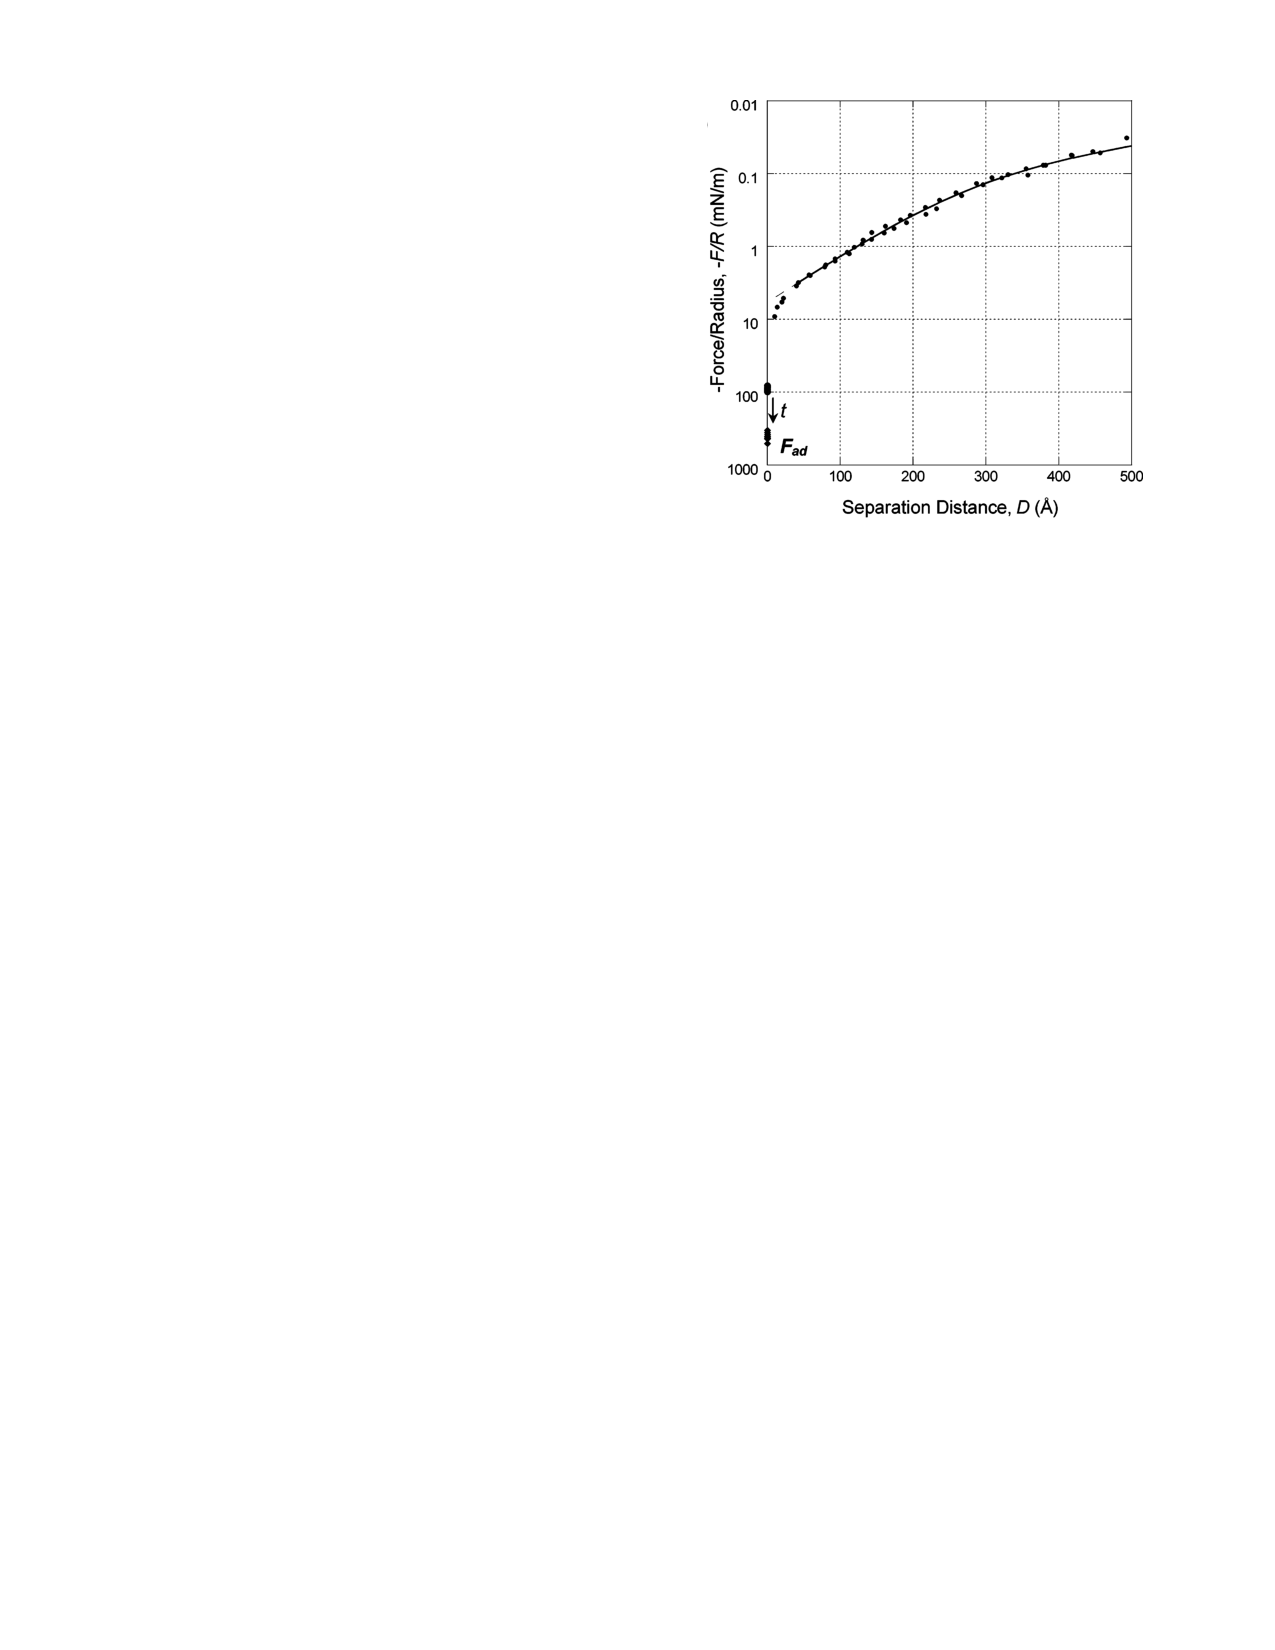
\includegraphics[width=0.35\textwidth]{figures/Background/LongRangeForce.pdf}
}
\caption{Force-distance curves for surfactant monolayers adsorbed on mica
reveal a lon-range attraction 
\cite{Lin2005}.
}
\label{fig:chandler_weeks}
\end{wrapfigure}
The hydrophobic attraction theory concerns the 
self-organization of hydrophobic particles in a viscous solvent.  
It is a phenomenological model mimicking 
the linear-response of water to surface perturbations
and was first proposed by applied mathematician 
Stjepan Mar\v{c}elja from the Australian National University in 1976.  
To explain certain repulsion measurements between lecithin bilayers,
Mar\v{c}elja and coworkers devised a mathematical
model using a Landau expansion of the free energy density 
of an order parameter for the orientation of water
\cite{LeRaPa77, MaRa76, LANDAULIFSHITZ5}.   
Their truncated free energy lead to a boundary value problem 
readily solved in terms of hyperbolic trigonometric functions
and ready 

Although simplistic, the model was general enough to 
explain a number of physical effects. 
For one, the mean orientations of water 
being opposite at the two interfaces yielded a
free energy that decreases with distance of separation
thus explaining the repulsion data for lecithin bilayers.  
Later, \cite{ClCh88,RaDe88} showed there was a 
long-range attractive force 
between hydrocarbon coated mica sheets 
following an exponential curve
and measurable up to 100 nm.  
\cite{ErLjCl89} applied the Mar\v{c}elja theory to this problem 
for an order parameter representing the excess number of
hydrogen bonds per water molecule.  

\begin{wrapfigure}[10]{r}{0.3\textwidth}
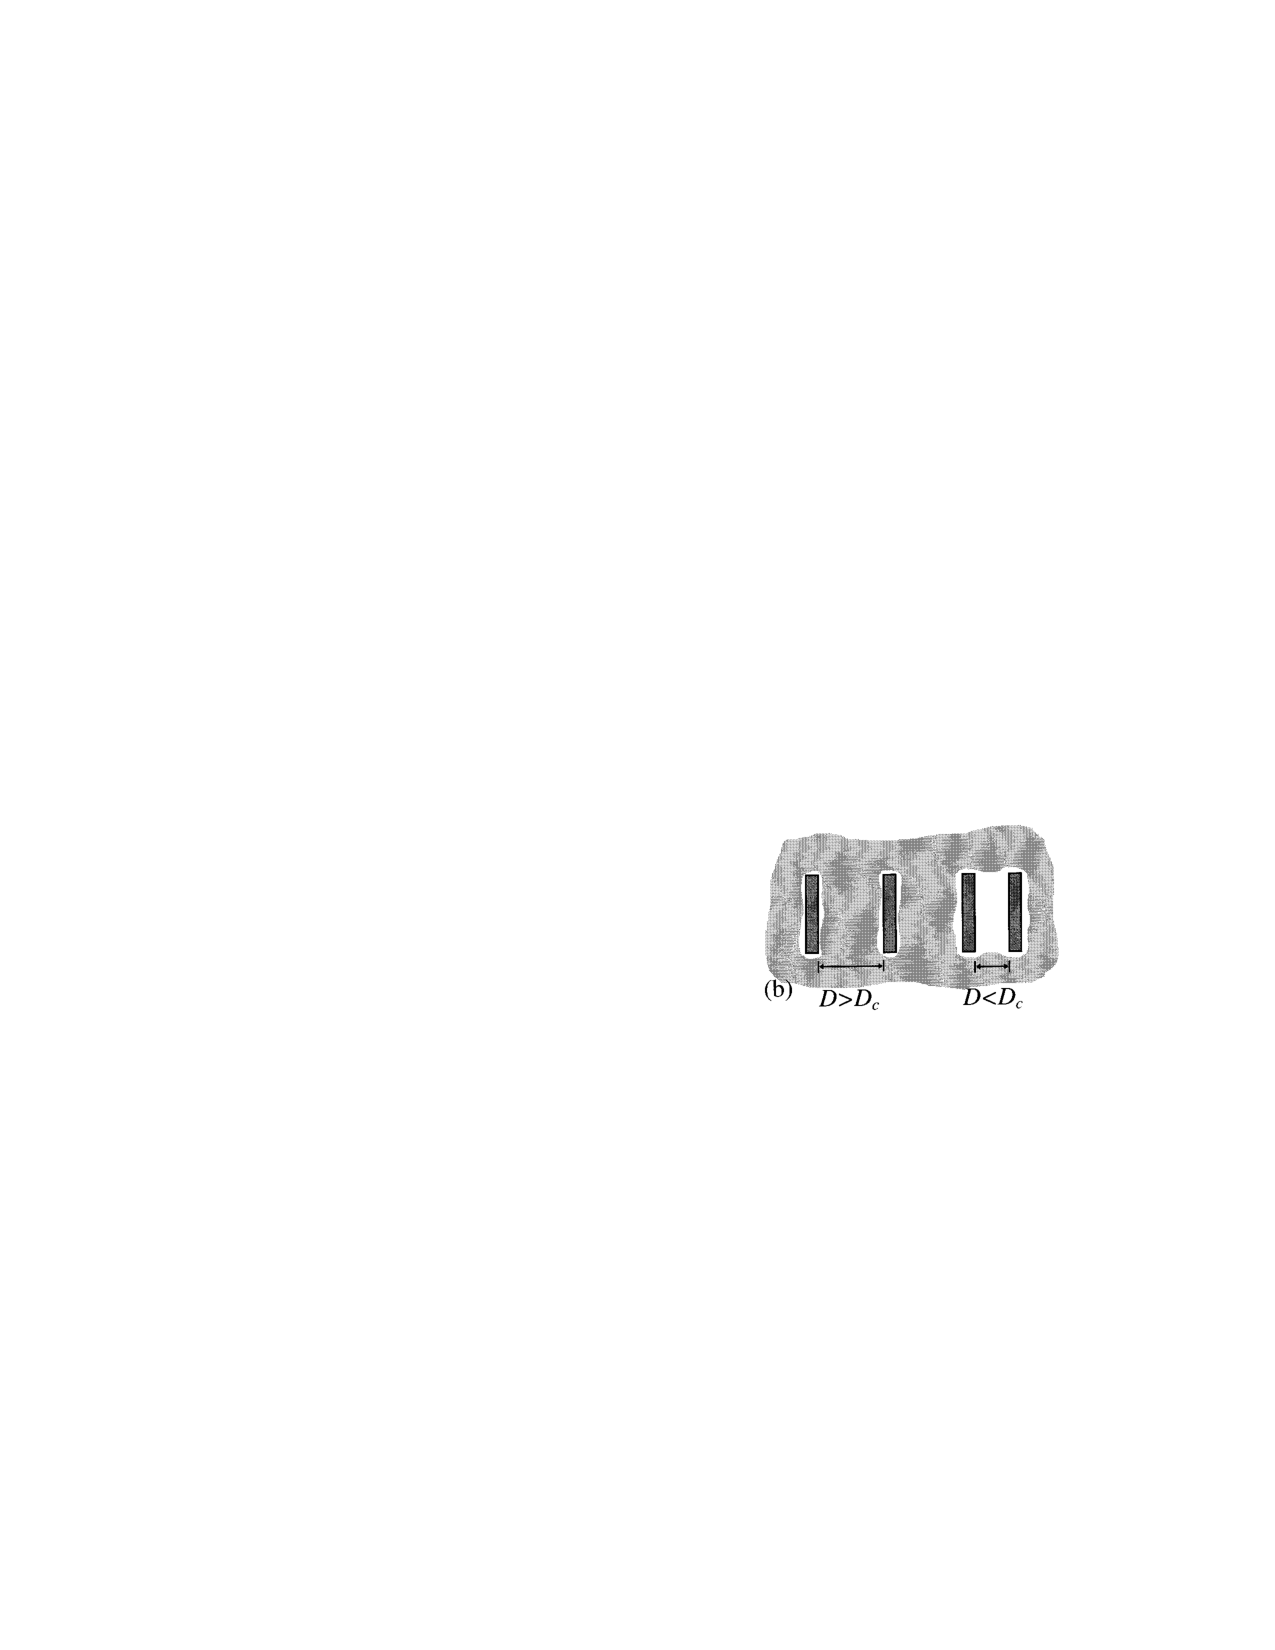
\includegraphics[width=0.3\textwidth]{figures/Background/ChandlerWeeks.pdf}
\caption{ Other theories explain hydrophobic attraction in
terms of the free energy of voids \cite{Lum1999}.
}
\label{fig:chandler_weeks}
\end{wrapfigure}
Analogues of Mar\v{c}elja's phenomenological theory 
show up in other areas related to biological self-assembly,
such as interaction of membrane-bound proteins 
\cite{KoNa15, Nagle17, KUZMIN2005}
and P. G. de Gennes's theory for the
interaction of polymer beads in mixed solvents \cite{deGe76}.
In the latter, the free energy corresponds to the
Ornstein-Zernike form of the order parameter correlation function.  
On the down side, it applies a continuum theory to
distances of a few molecular diameters, the association of
order parameter is arbitrary, it predicts monotonic forces,
and finally measured attractive forces amplify at distances below
10 nm and this feature is not accounted for by the theory
\cite{Ni80}.


\begin{wrapfigure}[22]{l}{0.3\textwidth}
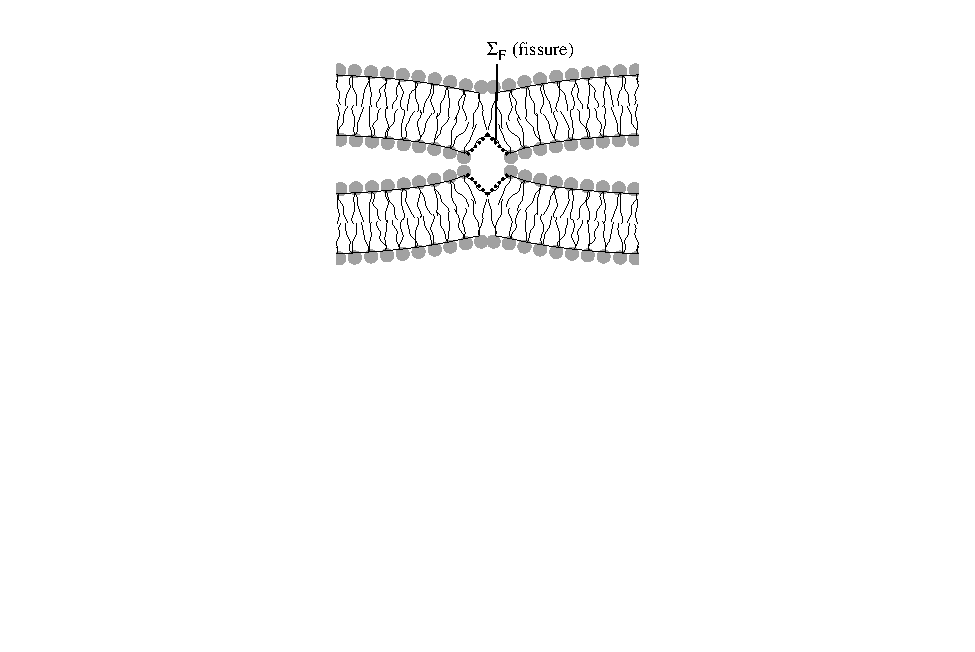
\includegraphics[width=0.3\textwidth]{figures/Background/Fissure.pdf}
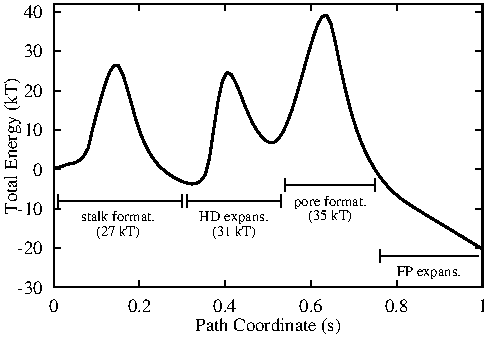
\includegraphics[width=0.3\textwidth]{figures/Background/Landscape.pdf}
\caption{
In fusion, fissures in the phospholipid monolayers expose hydrocarbon to water (top).
The energy of fissures dominates first and third stages of fusion (bottom).
}
\label{fig:fissure}
\end{wrapfigure}
Still, no single theory has beenable to account, either qualitatively or quantitatively,
for hydrophobic interaction over the full distance regime \cite{Lin2005, Meyer2006,Ducker2016}.
Despite the ubiquity of the phenomenon, theoretical developments explaining
the basic underlying principles of the hydrophobic effect have
come relatively late \cite{Ch05}. For example, studies of the partitioning of
hydrophobic solutes between water and nonpolar solvents provide
estimates for the energy cost of creating 
hydrophobic-water contacts that is a factor of three lower than
the value derived from interfacial tension measurements. Only
recently was an explanation for this discrepancy provided
\cite{Jackson2016}.

Whatever the case may be, the continuum approaches to water
structure that we present here are a conceptual advance 
that are further justified a posteriori from 
the agreement between theory and experimental surface force
curves. Researchers have used  Mar\v{c}elja's theory to calculate
energies of pore formation and fusion
\cite{Gletal88, Aketal17, RyKlYaCo16}. 
When open, the attraction between apposing hydrophobic surfaces
causes the fissure to collapse.
PI RR calculated energy barriers
of fusion using a modified form of the Helfrich
energy to include Mar\v{c}elja's free energy for the structure of 
water separating the fissures \cite{RyKlYaCo16}.
This value was later experimentally corroborated 
(Figure \ref{fig:fissure}, \cite{FrRoPi17}).

In summary, the consensus is that despite its apparent simplicity,
the predictions of the hydrophobic attraction theory are compatible
with experimental measurements and may closely reproduce the reality
of the physical process at a molecular scale \cite{FrRoPi17, Fretal21}.

In terms of applications, the approach resolves 
certain issue in soft matter modeling.
For example, the Helfrich hamiltonian from membrane biophysics
assumes a rod-like continuum but makes no use of the
amphiphilic character or lipids
\cite{Hamm2000, TerziDeserno17, PhysRevE.102.042406}.  
By coarse-graining lipids as Janus particles, we
derive the bilayer structure and elastic energies
from the amphiphilic character of constituent particles.
Moreover, the granularity of proteins and topological changes e.g.
protein induced curvature, fission, fusion, are
critical to understanding mechanical properties of membranes. 
These processes can be
modeled by standard continuum methods only with great difficulty and
excessive grid refinement.
%Assuming the location of pore nucleation,
%for example, is required in traditional continuum but is yet another
%output of our model. 
Finally, the methodology allows evolutions equations to be
computed using integral equation
methods that when optimized have near-linear in the particle number. 
%For comparison, that is the same computational cost as a finite element
%analysis of a two-dimensional membrane that ignores water.

%%%%%%%%%%%%%%%%%%%%%%%%%%%%%%
%
% The following commented out on Nov 6, 2021
%
%%%%%%%%%%%%%%%%%%%%%%%%%%%%%%%
%\section{Background}
%\label{sec:background}
%The goal of this collaborative proposal is to use mathematical modeling
%and numerical simulations to investigate the dynamic self-assembly of
%amphiphilic particles interacting via hydrophobic forces
%in solvent. Amphiphilic particles (such as lipid molecules) possess
%both hydrophobic and hydrophilic structures. In a viscous solvent they
%self-assemble into meso-/macroscopic structures (such as micelles and
%bilayers of lipids) to shield their hydrophobic parts from contact with
%the solvent (water) molecules.
%%
%%\subsection{Hydrophobic Forces}
%%\label{sec:hydrophobicforce}
%%
%Such self-assembly of amphiphiles via hydrophobic forces is ubiquitous in biology and biophysics \cite{Israelachvili1954},
%%The hydrophobic force is a ubiquitous molecular interaction in biology \cite{Israelachvili1954}, 
%and has been a major source of nonspecific interactions between
%nanoparticles in soft matter
%\cite{Sanchez-IglesiasEtAl2012_ACSNano,AltantzisEtAl2013_PSC,XieYangLuEtAl2020_COCIS}. 
%%The proposed research aims to provide fundamental understanding of the self-assembly dynamics of amphiphilic particles so to design smart materials of desirable properties by
%%tuning the geometry and properties of the amphiphilic particles. 
%
%%The hydrophobic force arises when polar solvent molecules come in contact with a non-polar substance, such as hydrocarbon or vapor.
%%In a polar solvent (like water), the dipole-dipole interaction between solvent molecules form a loosely structured hydrogen-bond network where
%%each solvent molecule shares bonds with neighboring molecules at any given time 
%%\cite{Israelachvili1954}. In the presence of  a non-polar solvent molecule loses the ability to form hydrogen bonds
%%in one direction. 
%%The decrease in the number of hydrogen bonds causes a reorientation, or structural
%%change, in the surrounding water that is energetically very unfavorable \cite{Bjorneholm2016}.
%
%
%The substantial free energy for placing hydrophobic substances in contact with water 
%is roughly proportional to the surface area of the contact region \cite{Bjorneholm2016}.  
%%As a result, hydrocarbon solutes have a large interfacial tension 
%%and try to minimize their surface area when in water. 
%At the microscopic level, the hydrophobic force is a long-range, surface
%interaction. This means that two hydrophobic surfaces, separated by
%water over some distance, experience an attractive force
%\cite{Lum1999,Meyer2006,Hammer2010}. Measurements show that the
%hydrophobic force decays exponentially with a decay length on the order of 1 nm
%\cite{Israelachvili1984, Marcelja1977,Christenson2001,Lin2005}. 
%Additionally, the interaction is not pairwise additive, meaning that
%the force between any two hydrophobic objects is altered by the presence
%of a third object, hydrophobic or otherwise \cite{SilveraBatista1242477}. 
%
%Recently, PIs RR and YNY developed a mathematical model, called the
%hydrophobic attraction potential (HAP) model \cite{Fu2018_SIAM}, that is based
%on the physical origin of hydrophobicity. This model addresses the major
%shortcomings of molecular dynamics (MD) and continuum approaches. Based
%on preliminary results (\S\ref{sec:preliminary_work}), the PIs propose to
%extend this HAP model to offer an alternative modeling methodology that
%leads to new mathematical ideas and is both physically accurate and
%computationally practical.
%%
%%
%%The word hydrophobic (water fearing) derives from the low solubility of oil (hydrocarbon solute) in water and vice versa. 
%%It causes hydrophobic moieties to aggregate and cluster,
%%is responsible for the adhesion between hydrophobic surfaces \cite{Ducker2016}, large contact angles on a 
%%dewetting surface \cite{Arenas2019,Sandre1999}, accumulation of particles along interfaces \cite{Lee2013,Lee2014}, 
%%formation of micelles and bilayers \cite{Israelachvili80}, and protein folding and membrane insertion \cite{Kabelka2018}.
%%
%%Lipids are amphiphilic molecules whose  structure possesses
%%both hydrophobic and hydrophilic parts. 
%%The amphiphilic property is what allows lipids to form the membranes and 
%%compartments of living cells \cite{Israelachvili80}. 
%%More specifically, a lipid consists of 
%%an elongated hydrocarbon tail that is hydrophobic, attached to a polar head that is hydrophilic.
%%To shield the hydrophobic tails from water, lipids self-assemble into micelles and bilayers. 
%%A micelle is a spherical arrangement of lipids with tails terminating at the micelle center. 
%%A bilayer consists of two layers of lipids called monolayers, where the lipid tails point 
%%from the monolayer surface into the bilayer core. 
%%
%%The mathematical modeling of a biological membrane is a challenging problem in applied mathematics. 
%%Bilayers are elastic and resist deformations like bending, twisting, and stretching.
%%Their elastic deformations are well described by the theory of liquid crystals \cite{ANDRIENKO2018520}.
%%Lipid bilayer membranes can also be fluidic, and the lateral translation of lipids (or any membrane bound
%%proteins) couples nonlocaly to the motion of the aqueous environment \cite{MerkelSackmannEvans1989,StoneAjdari1998_JFM,OppenheimerDiamant2009_BJ,OppenheimerDiamant2011_PRL}. 
%%%Finally, the membranes of cellular 
%%%compartments are constantly merging and pinching as part of intracellular trafficking. 
%%%Therefore monolayer surfaces undergo discontinuous deformations. 
%%
%%There are two prevailing approaches in membrane modeling, and each has its advantages
%%and disadvantages. Molecular dynamics (MD) is to date the only tool capable of resolving granular biological details
%%The computational cost of MD, however, grows with the sixth power of the sample diameter and 
%%so simulations are severely limited to 
%%small system sizes and short time scales \cite{DiCarlo2019}.
%%The other approach, continuum mechanics, assumes smooth surfaces and can therefore model 
%%realistic systems over physical times. 
%%But continuum description of a biological membrane ignores the granularity of lipid molecules, and thus requires some assumptions when a
%%membrane ruptures or when two membranes fuse \cite{ChKo08}. 
%%%
%%%mechanics presumes, rather than predicts, the nucleation of discontinuities. 
%%%
%%
%The proposed research aims to provide fundamental insight into the
%self-assembly dynamics of amphiphilic particles. These results will
%facilitate optimal design of smart materials by tuning the geometry and
%properties of the amphiphilic particles.
%
%
%\begin{wrapfigure}[9]{r}{0.24\textwidth}
%  \vspace{-20pt}
%\centerline{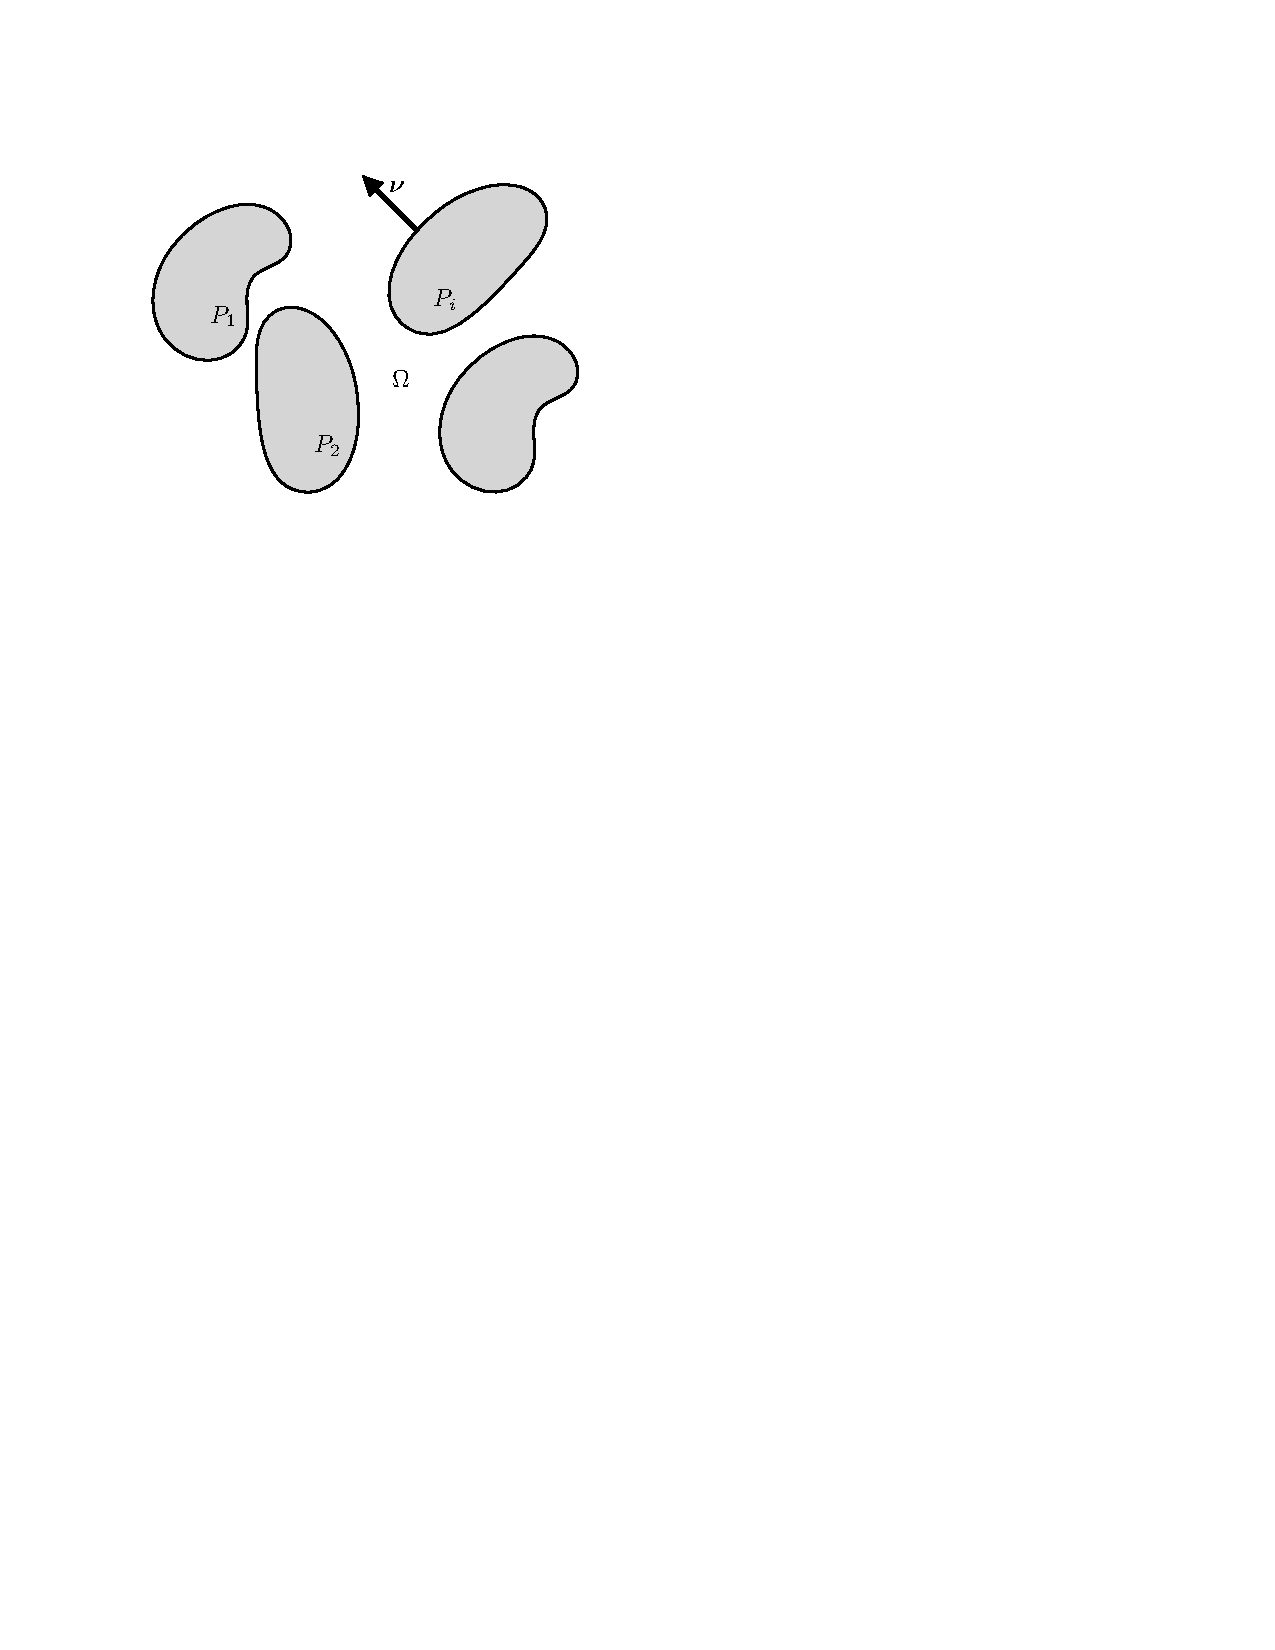
\includegraphics[width=0.23\textwidth]{figures/BG_fig1.pdf}}
%\caption{ \footnotesize
%A collection of rigid particles: $P_1,$ $P_2,$ $P_3, \ldots$. The
%exterior domain $\Omega$ represents the solvent.}
%  \label{fig:domain}
%\end{wrapfigure}
%\subsection{Hydrophobic Attraction Potential (HAP)}
%\label{sec:HAP}
%%Based on the physical origin of hydrophobicity,  we have devised a
%%functional, called the hydrophobic attraction potential (HAP), to model
%%hydrophobic forces~\cite{Fu2018_SIAM}. 
%The motivation for the HAP concept stemmed from PI RR's work concerning
%energy barriers in membrane
%fusion~\cite{RyKlYaCo16,Chetal16}. By applying a mathematical, squared-gradient
%theory for hydrophobic attraction between planar
%surfaces~\cite{Eriksson1989,Lum1999,Menshikov2017,Marcelja1977}, PI RR
%and collaborators resolved the long-standing issue of accounting for the
%energy of a monolayer fissure surface during topological transitions.
%Based on PI RR and YNY's coarse-grained membrane modeling
%work~\cite{Fu2017}, the investigators devised a gradient theory for
%arbitrary collections of hydrophobic and
%amphiphilic particles. As a new method, HAP eliminates the costly calculation
%of water by treating the solvent implicitly, is capable of representing
%biologically-relevant morphologies, and avoids complicated
%re-meshing schemes of continuum approaches by utilizing a particle-based
%representation.
%
%To define HAP, consider a collection of particles suspended in a
%solvent. The region $\Omega \subset \mathbb{R}^3$ models the solvent
%phase (Figure \ref{fig:domain}).
%%The HAP must be an energy of the shape of the region because hydrophobic
%%attraction is non-additive.
%The boundary of the region is the union of water-particle interfaces
%with unit normal $\boldsymbol{\nu}$. Some parts of this interface are
%hydrophobic while others are hydrophilic. Hydrophobic interfaces disturb
%the hydrogen bond structure of water~\cite{Luzar1987, Jonsson2006,
%Varilly2011} and this disturbance comes with an energetic penalty that
%is proportional to interfacial area. There is an additional decay
%length, due to rapid fluctuation in the hydrogen bond network,
%describing how far the restructuring extends into bulk water.
%
%The above considerations motivate the following definition for HAP:
%\begin{align}
%\label{HAP}
%  \Phi = \gamma \int_{\Omega} \rho |\nabla u|^2 + \rho^{-1}u^2 \,\dif V. 
%\end{align}
%The integrand contains
%the decay length $\rho$
%and a dimensionless scalar function $u(\mathbf{x})$ called the water activity.
%The integrand has units of an inverse length, so
%the volume integral has units of area. Multiplication by interfacial tension
%$\gamma$ makes $\Phi$ an energy. 
%
%To establish an attraction between interfaces, the water activity is not
%arbitrary but rather is the solution of the screened Laplace
%equation boundary value problem 
%\begin{equation}
%  \label{SL}
%  -\rho^2 \Delta u + u = 0, \mbox{ } \mathbf{x} \in \Omega, \qquad
%  u = f,  \mbox{ } \mathbf{x} \in \partial \Omega, \qquad 
%  u(\mathbf{x}) \to 0, \mbox{ as } |\mathbf{x}| \to \infty.
%\end{equation}
%The boundary values $f$ define the degree of hydrophobicity of the
%water-particle interface: $f=1$ describes a hydrophobic interface, and
%$f=0$ describes a hydrophilic interface. Thus, $f$ encodes information
%about the particles, and the parameters $\rho$ and $\gamma$ encode
%information about the quality of the solvent~\cite{Israelachvili1954,
%Discher2002}.
%In the figures throughout the proposal, red is for $u = 1$ and blue is for $u = 0$.
%In practice, we integrate~\eqref{HAP} by parts and
%use~\eqref{SL} to obtain
%\begin{equation}
%\label{eq:HAP_easy}
%\Phi = -\gamma \int_{\partial \Omega} \rho u \nabla u \cdot \boldsymbol{\nu} \,\dif S,
%\end{equation}
%thereby avoiding volume integral calculations.
%
%The equations~\eqref{HAP} and~\eqref{SL} possess a number of
%mathematical properties that mirror the phenomenological characteristics
%of hydrophobic attraction. Specifically, solutions of~\eqref{SL} yield
%an attractive force between hydrophobic bodies separated by water, and
%this attraction decreases exponentially with the distance of
%separation~\cite{Eriksson1989}. Using boundary layer analysis, the HAP
%converges to a surface energy in the zero-decay length
%limit~\cite{Lee2018, Lin2015, Shibata2004}. Finally, we have
%demonstrated that the forces derived from HAP theory are
%non-additive~\cite{Meyer2006, Fu2018_SIAM}. 
%%The hydrophobic force has been implicated in the directed folding of proteins, 
%%adhesion between biological membranes, but it is still unanswered as to whether
%%the hydrophobic force of the form (\ref{HAP}--\ref{SL}) exists between small molecules. 
%
%%As a summary of its mathematical properties,  the hydrophobic force
%%is a non-additive, exponentially decaying surface force 
%%that possesses a separation of length scales. These properties suggest 
%%a boundary value problem formulation of the hydrophobic force.  
%%The non-additivity of the hydrophobic force has to do with the fact that there is no superposition
%%principle for including subdomains in boundary value problems. 
%%The exponential decay is a property of a second order elliptic partial differential equation (PDE). 
%%Finally, the separation of scales come from boundary layers, 
%%where the energy of the boundary layer in the zero-thickness limit corresponds to macroscopic interfacial tension.
%%Overlapping boundary layers correspond to microscopic hydrophobic attraction, 
%%and the boundary layer thickness corresponds to the decay length of attraction.
%%
%%
%%\section{Previous Results by the PIs}
%%\label{sec:results}
%%
%%%In our paper \cite{Fu2018_SIAM}, 
%%PIs RR and YNY developed the HAP model (\ref{HAP}--\ref{SL})
%%to quantify the macroscopic assembly and mechanics of a lipid bilayer membrane in solvents \cite{Fu2018_SIAM}.
%%%We formulated the boundary value problem as a second-kind
%%%integral equation (SKIE), presented in the Section (). 
%%%The simulated fluid-particle systems exhibit a variety of multiscale behaviors over both time and length.
%%%Over short time scales, the numerical results showed self-assembly for model lipid particles. 
%%%For large system simulations, the particles formed realistic configurations like micelles and bilayers. 
%%%Our collections showed that these amphiphilic particle bilayers  possessed mechanical properties of a 
%%%lipid  bilayer  membrane  that  are  consistent  with other results in the literature.   
%To define the particle dynamics, let $P_1$, $P_2$, \ldots, $P_N$ be a
%finite collection of disjoint, rigid, and closed particles each with
%a Lipschitz boundary. Assume that the label $f$ is an element of the
%Sobolev space $H^1(\Omega)$. The functional~\eqref{HAP} has a minimizer
%among all functions $u$ equaling $f$ on the boundary in the sense of
%trace. Conversely, from maximum principles and energy estimates, the
%solution of~\eqref{SL} is unique and minimizes~\eqref{HAP}. Taking the
%first variation of~\eqref{HAP}, i.e.~the derivative with respect to the
%domain~\cite{Bandle2015, Schiffer1954, Grinfeld2010}, yields a
%symmetric, rank-two tensor called the hydrophobic stress (equation (2.3)
%in~\cite{Fu2018_SIAM}):
%\begin{align}
%  \label{stress}
%\boldsymbol{\sigma}_{\text{hydro}} = \gamma \rho^{-1} u^2 I + 2\rho
%  \gamma \left(\frac{1}{2}|\nabla u|^2I - \nabla u \nabla u^T\right).
%\end{align}
%%
%%To obtain \eqref{stress}, we observe that the potential $\Phi$ is a function of the particle position and orientations.
%%This is because the particle configuration defines the shape of $\Omega$ and the boundary data $f.$ 
%%Taking the derivative of \eqref{HAP} with respect to particle configurations, and using the boundary value problem \eqref{SL}
%%in a critical way leads to the surface term \eqref{stress}.  
%%
%Integrating the hydrophobic stress over the surface of particle $P_i$
%reveals the hydrophobic force, and torque on each particle 
%\begin{align}
%  \label{forceandtorque}
%  \mathbf{F}_{\text{hydro},i} = \int_{\partial P_i} \boldsymbol{\sigma}_{\text{hydro}}
%  \cdot \boldsymbol{\nu} \,\dif S,\quad
%  \mathbf{G}_{\text{hydro},i} = \int_{\partial P_i} (\mathbf{x}-\mathbf{a}_i) \times
%  (\boldsymbol{\sigma}_{\text{hydro}} \cdot \boldsymbol{\nu}) \,\dif S,
%\end{align}
%relative to the center of mass $\mathbf{a}_i$. This system is force- and
%torque-free (\S\ref{subsec:specific_aim_2}). To avoid particle
%collisions, we define an excluded volume potential $\Phi_{\text{repul}}$
%that diverges whenever tubular neighborhoods of adjacent particles
%overlap. The total potential, force, and torque are then
%\begin{equation}
%\label{eq:total_poten}
%\Phi = \Phi_{\text{hydro}} + \Phi_{\text{repul}},\quad
%\mathbf{F}_{i} = \mathbf{F}_{\text{hydro},i} + \mathbf{F}_{\text{repul},i},\quad
%\mathbf{G}_{i} = \mathbf{G}_{\text{hydro},i} + \mathbf{G}_{\text{repul},i}.
%\end{equation}
%
%To supply viscous dissipation, we incorporate the mobility problem
%flow for a rigid body suspension in Stokes flow:
%\begin{equation}
%\label{eq:stokes}
%\begin{aligned}
%  &-\mu \Delta \mathbf{u} + \nabla p = 0, \quad \mathbf{x} \in \Omega, \qquad 
%  \nabla \cdot \mathbf{u} = 0,  \quad \mathbf{x} \in \Omega,\\
%  &{\bf u}(\mathbf{x}) \to 0 \quad \text{as}\ |\mathbf{x}|\to \infty,\qquad 
%  \mathbf{u}(\mathbf{x})|_{\partial P_i} = \mathbf{v}_i +
%\boldsymbol{\omega}_i\times(\mathbf{x} - \mathbf{a}_i),\\
%&\int_{\partial P_i}\boldsymbol{\sigma}\cdot {\bf n} \dif S=-{\bf F}_i, \quad
%\int_{\partial P_i} (\mathbf{x} - \mathbf{a}_i)\times (\boldsymbol{\sigma} \cdot \mathbf{n}) \dif S =-{\bf G}_i.
%\end{aligned}
%\end{equation}
%Here, $\mu$ is the fluid viscosity; the first two equations state that
%the fluid motion is a divergence-free Stokes flow; the third equation
%specifies that the fluid velocity vanishes at infinity; the fourth
%equation enforces a rigid body motion on each particle, where
%$\mathbf{v}_i$ and $\boldsymbol{\omega}_i$ are unknown translation and
%angular velocities; and the last two equations state that the net
%viscous forces and torques with fluid shear stress $\boldsymbol{\sigma}$
%balance \eqref{eq:total_poten}.
%
%
%The time integration of particle configurations goes as follows:
%\textbf{(i)} solve the BVP~\eqref{SL} for the screened Laplace equation,
%\textbf{(ii)} determine the rigid body forces and
%torques~\eqref{forceandtorque}, \textbf{(iii)} solve the Stokes mobility
%problem~\eqref{eq:stokes} for the rigid body motions, and \textbf{(iv)}
%update the particle configuration.  Numerical challenges and how these
%challenges are overcome are described in \S\ref{subsec:specific_aim_2}.
%
%%%(2YY: 
%%We have intentionally ignored  latency in the variational 
%%calculations. At issue is that any change in the particle position involves the relaxation time 
%%of the hydrogen bond network. To remedy this, we could parametrize a path for the 
%%particles configuration as a function of physical time. Then the rate of change
%%of hydrophobic interaction includes the surface hydrophobic stress as calculated, but also a body term 
%%for time change of activity, assuming we model hydrogen bond relaxation by diffusion. 
%%The diffusion time, however, is extremely small since hydrogen bond lifetimes are on the order 
%%of $10^{-11}$ s \cite{Israelachvili1954}. This setup is analogous  to that of a Kelvin-Voigt material,
%%where viscoelastic deformations exponentially approach the purely elastic deformation.  
%%%)
%
%\begin{wrapfigure}[14]{l}{0.35\textwidth}
%\centerline{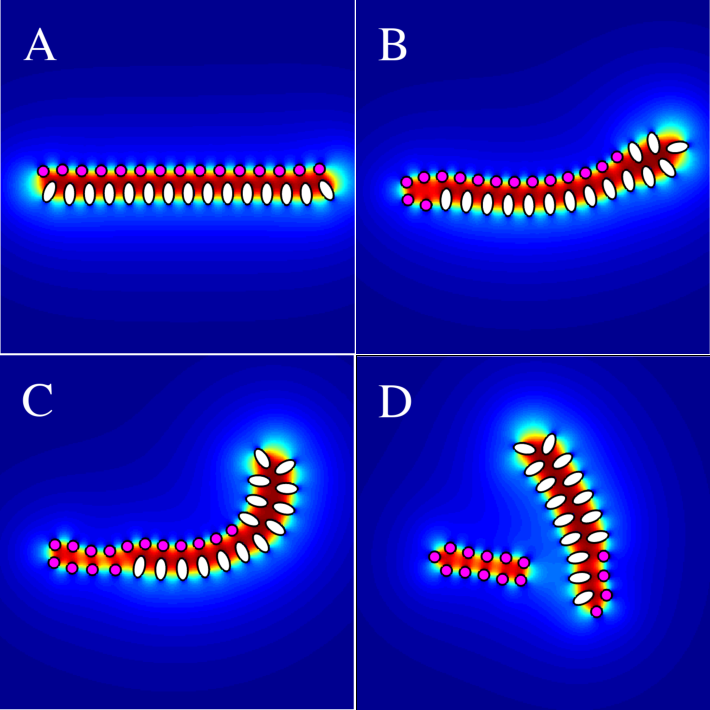
\includegraphics[width=0.34\textwidth]{figures/PW_fig2.pdf}}
%  \vspace{-8pt}
%  \caption{\label{fig:demixing} \footnotesize An initial assembly of
%  small and large particles spontaneously segregates into two smaller
%  bodies.}
%\end{wrapfigure}
%The HAP formulation is, to our knowledge, the first demonstration of
%bilayer self-assembly by a continuum-based interaction
%model~\cite{Noguchi2001, Farago2003, Brannigan2006, Brooks2009,
%Wang2013}. Our simulations use Janus particles to model lipid
%amphiphiles which are popular in material science and physics for
%creating functional materials~\cite{Lee2014, Lee2013}. Janus particles
%are typically spherical with a biphasic material label on either
%hemisphere, endowing the particle with
%a directional order. We model an
%elongated lipid by elliptical particles with the hydrophobic label
%defined along the ellipse's axis. 
%Under the hydrophobic force, with
%excluded volume, the Janus particles spontaneously merge and realign
%to form bilayers. This occurs only as a result of energy minimization
%and does not require artificial inputs.
%%
%
%%
%It is worth emphasizing that the HAP model uses only a few parameters:
%interfacial tension, decay length, repulsion strength, and particle
%shape. For example, an elastic modulus for stretching a vesicle from
%micropipette manipulation calibrates our interfacial tension
%parameter. This is in direct contrast with pair-potential-based
%approaches in MD simulations and coarse-grained models where many more
%parameters are required~\cite{Varilly2011, Wang2013}.
%%MD simulators have also made measurements and lately there is better and better agreement with reality. 
%%But even the simplest coarse grained models based on pair potentials for lipids has many more parameters \cite{Varilly2011,Wang2013} . 
%
%%As a proof of concept, our work has already tested for elastic energies
%%for bending, stretching, and tilt of the bilayer assembly. The elastic
%%coefficients derived from the HAP simulations show strikingly positive
%%agreement with experimentally determined values~\cite{Fu2018_SIAM}.
%%Encouraged by these results and the hydrodynamic simulations of
%%bilayer assembly, the PIs propose to extend the HAP model to make direct
%%comparisons with experimental results \S\ref{subsec:specific_aim_1} and to
%%establish that the HAP model has the capability to model
%%flow phenomena across length scales and time scales
%%\S\ref{subsec:specific_aim_2} using efficient, high-order numerical
%%methods \S\ref{subsec:specific_aim_3}.
%
%%\begin{wrapfigure}[14]{l}{0.35\textwidth}
%%\centerline{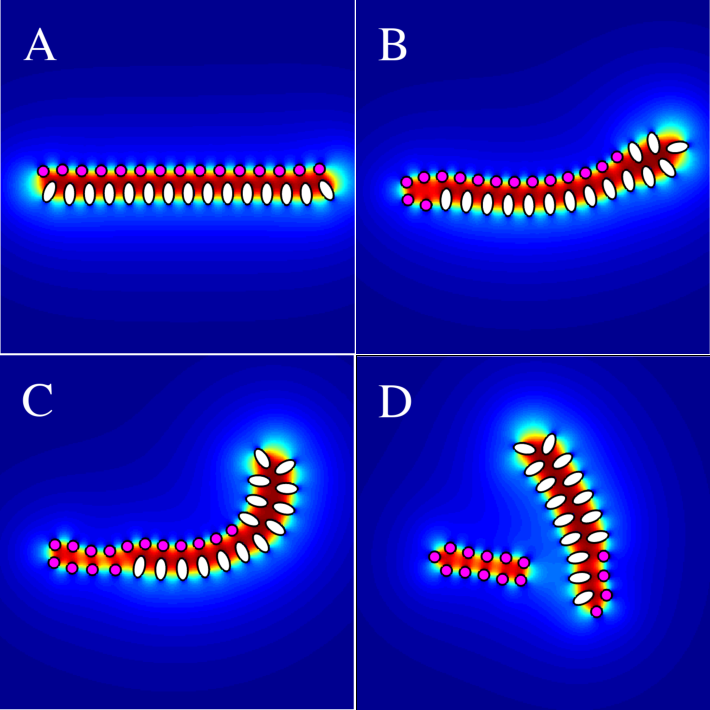
\includegraphics[width=0.35\textwidth]{figures/PW_fig2.pdf}}
%%  \vspace{-8pt}
%%  \caption{\label{fig:demixing} \footnotesize An initial assembly of
%%  small and large particles spontaneously segregates into two smaller
%%  bodies.}
%%\end{wrapfigure}
%Over the past decades, researchers have used a number of mathematical
%tools to simulate vesicles in a shear flow, including lattice
%Boltzmann~\cite{KaouiHartingMisbah2011_PRE}, coarse-grained Brownian
%dynamics~\cite{NoguchiTakasu2002_BJ}, phase
%field~\cite{DuLiuWang2004_JCP,BibenKassnerMisbah2005_PRE}, level
%set~\cite{DoyeuxGuyotChabannesEtAl2013_JCAM}, boundary
%integral~\cite{Shravan09,Rahimian15}, and immersed boundary
%approaches~\cite{KimLai2010_JCP,KimLai2012_PRE,HuLaiSeolEtAl2016_JCP}.
%Most of these approaches assume a mathematical surface, whether
%implicitly or explicitly, and define an elastic bending energy of the
%surface. These vesicle studies built off of numerical methods for
%calculating energy minimizing steady equilibrium shapes of lipid bilayer
%membranes, vesicles, and red blood cells. These approaches range from
%the finite element~\cite{Bartels,Peng13,RyKlYaCo16,Sinha15},
%phase field~\cite{Du05,QiangDu08,Lowengrub13}, and immersed
%boundary methods~\cite{Hu,Hu13, KimLai2010_JCP}. PI RR and collaborators
%led in part the development of phase field functionals of membrane
%elastic energy and approaches to coupling membrane elasticity to
%fluids~\cite{0951-7715-18-3-016,Du05,DuEuler,QiangDu09}.
%
%
%%The vesicle obeys fluid
%%transport and in turn the fluid balances shear stress with the vesicle's bending force. 
%
%Our HAP approach differs from these prior methods in a number of
%respects. First, we do not assume a surface. Rather, we 
%assume a collection of amphiphilic particles. The
%collection of amphiphiles minimize hydrophobic interactions by
%sequestering hydrophobic tails in the form of a bilayer, and the
%particles' excess free energy gives rise to an elastic bilayer energy.
%The second difference lies in the fluid-interface coupling. Here, the
%associated mobility problem~\eqref{eq:stokes} is more complicated than
%dealing with a stress boundary condition or diffusive surface force
%because the fluid velocities are for individual rigid body motions at each
%particle surfaces. Finally, the HAP model directly addresses the
%existence of multiple phases. We can vary lipid length, spontaneous
%curvature, and bending rigidity by introducing different particle shapes
%and hydrophobic boundary conditions (Figure~\ref{fig:demixing}). In
%contrast, continuum theory deals with multiple phases through additional
%surface densities that must satisfy specialized transport
%equations~\cite{Lowengrub07, MikuckiZhou17}. 
%
%
%\begin{wrapfigure}[6]{r}{0.35\textwidth}
%\centerline{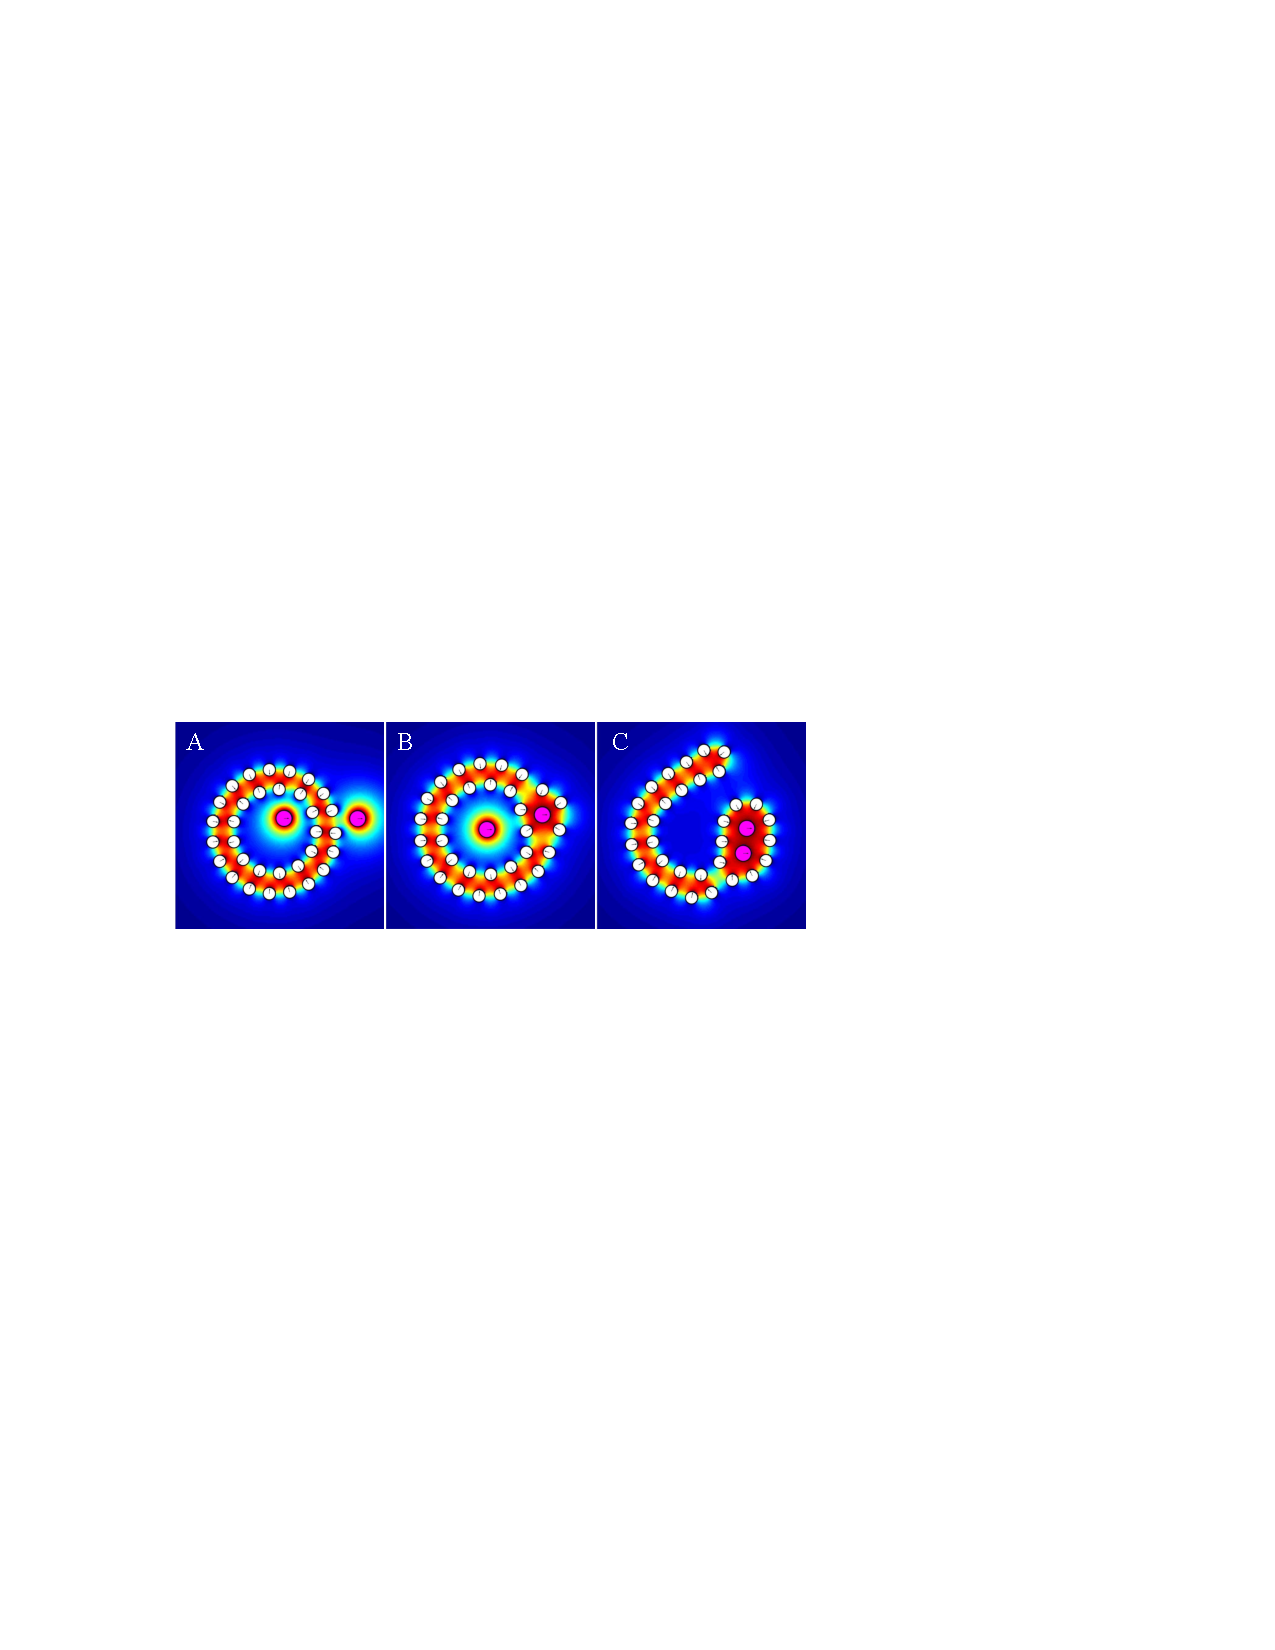
\includegraphics[width=0.34\textwidth]{figures/Lysis.pdf}}
%  \vspace{-8pt}
%  \caption{\label{fig:lysis} \footnotesize Two hydrophobic particles
%  enter and then lyse the circular bilayer.}
%\end{wrapfigure}
%The greatest strength of using the HAP to model a lipid bilayer membrane is
%the ability to form discontinuities (interfacial singularities) from first
%physical principles without any artificial manipulation to rearrange the
%interface (Figures~\ref{fig:demixing} and~\ref{fig:lysis}). For
%example, using the HAP model to simulate a vesicle under a shear flow
%that is strong enough to cause the vesicle membrane to rupture (see
%\S\ref{sec:preliminary_work}), we expect the HAP model to capture the
%reorganization of lipid molecules on the scales of membrane thickness
%($\sim 5$ nm), which is a nearly impossible task using phase-field or
%immersed boundary methods without extreme refinement around the membrane
%and artificial treatment of reconnection during the topological change
%of an interface \cite{doi:10.1063/5.0009734, LiAn-Chang16,
%doi:10.1098/rspa.2012.0505, doi:10.1137/130941432, Feetzl18,
%doi:10.1137/16M1108406}.
%
%%Some disadvantages are that the hydrophobic interaction does not constrain vesicle volume. 
%%Instead, changes in volume are rate limited by inter-particle spacing,
%%which may be undesirable in case of a mathematically strict volume constraint.
%%% set vesicle volume, as is done in the study of liposomes
%%%using auxiliary constraint equations for instance. 
%%%Also, the boundary integral method formulation
%%%relies on linearity of the Stokes equations. There has been some progress in
%%%boundary integral methods for the non-linear Navier-Stokes equations [ref].
%%%We point out that some non-Newtonian effects in polymers are a consequence of hydrophobic
%%%and steric molecular interactions like the ones presented in this proposal. 
%
%
%
%
%
%%
%%
%%The next few years provide the ideal window of opportunity for demonstrating the physical realism 
%%of the HAP model. 
%%
%%
%%
%%The definitions and calculations for fully three-dimensional bilayer elastic energies are described in greater
%%detail in Specific Aim 1. 
%%
%
%
%% 4.1 pN / nm = 4.1 pN nm / nm^2 = 4.1(1e-12)(1e-9) N m/(1e-18) m^2 = 4.1 (1e-3) J/m^2 = 4 mJ/m^2 
%% pN/nm = mJ / m^2 and 1 kT / nm = 4 mJ / m^2 so stretching 40 gives 40  
%% erg / cm^2 =  (1e-7) J/(1e-4) m^2 =   1e-3 J/m^2 =  mJ/m^2  
%% 120 mJ / m^2 
%% 10 erg / cm^2 = 10 pN nm / nm^2 = 2 kT / nm^2 
%%
%
%%\section{Proposed Research}
%%\label{sec:proposed-work}
%%The goal of the proposed research is to develop fast,
%%high-order-accurate, parallel numerical algorithms for large-scale
%%simulations of the collective hydrodynamics of janus particles in a solvent in both two- and three-dimensions.
%%First we summarize some basic formulation and preliminary results
%%\cite{Fu2018_SIAM} in \S~\ref{subsec:bie} and \S~\ref{subsec:3dbie}.
%%We then describe outstanding numerical issues that we propose to address  in \S~\ref{subsec:proposed_research}.
%
%%\section{Proposed Research}
%%\label{sec:proposed-work}
%%The goal of the proposed research is to develop fast,
%%high-order-accurate, parallel numerical algorithms for large-scale
%%simulations of the collective hydrodynamics of  amphiphilic particles in a viscous solvent.
%%%
%%Based on the integral formulation in \S~\ref{subsec:bie} and \S~\ref{subsec:3dbie}, we have demonstrated that 
%%our potential theory approach can efficiently simulate self-assembly of 
%%amphiphilic particles into two-dimensional micelles, bilayer membranes,
%%and vesicles \cite{Fu2018_SIAM}.
%%%
%%While these results show great potentials in simulating the collective hydrodynamics of amphiphilic particles and
%%reproducing mechanical properties of their bilayer assembly, 
%%several outstanding issues need to be addressed for such approach to be efficiently applied to three-dimensional 
%%collective hydrodynamics of amphiphilic particles.
%%
%%the two-dimensional hydrodynamics of amphiphilic particles 
%%
%%the two-dimensional results in \cite{Fu2018_SIAM} are in agreement with the 
%%
%%
%%First we summarize some basic formulation and preliminary results
%%\cite{Fu2018_SIAM} in \S~\ref{subsec:bie} and \S~\ref{subsec:3dbie}.
%%We then describe outstanding numerical issues that we propose to address  in \S~\ref{subsec:proposed_research}.
%% -----------------------------------------------------------------------------
%%\subsection{Proposed research: High-order discretization of surface integrals in three dimensions}\label{subsec:proposed_research}
%%% -----------------------------------------------------------------------------
%%% {{{
%%The practical application of integral equation methods requires the
%%accurate evaluation of boundary integrals with singular, weakly
%%singular or nearly singular kernels.  Historically, these issues have
%%been handled either by low-order product integration rules (computed
%%semi-analytically), by local modifications of a smooth
%%rule~(e.g.~\cite{alpert,kapur,sidi}), by singularity
%%subtraction/cancellation (e.g.~\cite{duffy,bruno1,bruno2,davis_1984,graglia_2008,hackbusch_sauter_1994, jarvenpaa_2003,khayat_2005,kress_boundary_1991,schwab_1992, ying_2006}), by kernel
%%regularization and asymptotic analysis (e.g.~\cite{beale1,beale2,goodman_1990, haroldson_1998, lowengrub_1993,schwab_1992}), or by the
%%construction of special purpose ``generalized Gaussian'' quadrature
%%rules (e.g.~\cite{ggq1,ggq2,ggq3}).
%%In the complex analytic case, additional methods
%%have been developed by \citet{helsing_2008a} for off-surface
%%evaluation. It should be noted that in the two-dimensional case,
%%several of these alternatives provide extremely effective schemes,
%%especially the kernel-splitting method developed by Johan Helsing
%%\cite{helsing_integral_2009,helsing_tutorial_2012,helsing_2008a} since
%%they all permit local adaptivity and high order accuracy.
%%
%%The high-order quadrature rules for the evaluation of surface integrals
%%in three dimensions are much less developed than the line integrals in two
%%dimensions. For example, there are no Gaussian quadratures for integraing
%%polynomials on a flat triangle, even though efficient quadratures
%%\cite{xiao2010cma,vioreanu2014} have been
%%developed recently for such purpose. For weakly singular or singular integrals,
%%\cite{bremer2012jcp,bremer2013jcp} constructed high-order quadratures
%%for surface integrals on a general triangle, while \cite{gimbutas2013sisc}
%%presented a fast algorithm for integrating $1/r$-type singular integrals
%%for surfaces that are homeomorphic to a sphere. We would like to propose
%%to study the so-called quadrature by expansion (QBX) scheme~\cite{klockner2013jcp,qbx2}
%%for the evaluation
%%of both singular and near-singular surface integrals encountered in the
%%discretization of BIEs in three dimensions. Conceptually, the idea of the QBX
%%to evaluate singular, hypersingular and near singular integrals
%%on smooth surfaces is more or less straightforward. That is, the surface is discretized
%%into smooth triangles and smooth high-order quadratures are applied to evaluate
%%the expansion coefficients
%%on all source triangles with the QBX expansion center placed at a point off the surface.
%%One may then form a suitable expansion (for example, a Taylor expansion) around that
%%center and evaluate this expansion back at the target point on the surface (or close
%%to the surface in the near singular case). Compared to the competing aforementioned
%%quadrature schemes, the QBX quadrature is attractive
%%because it offers a clear path for being extended to: \textbf{(1)}
%%handle any ambient and source dimensionality, \textbf{(2)} integrate
%%any kernel, and thereby be usable for a very large range of PDEs and
%%boundary conditions, \textbf{(3)} handle any singularity, including
%%hypersingular operators, \textbf{(4)} be usable with any high-order surface
%%discretization, \textbf{(5)} generate well-conditioned discrete
%%operators to which iterative methods such as GMRES~\cite{gmres} can be
%%applied in a black-box fashion, \textbf{(6)} be computationally
%%efficient enough to be applied on the fly (without the need to store
%%quadrature tables), \textbf{(7)} integrate well with fast algorithms
%%such as the Fast Multipole Method. 
%%
%%In practice, there are still many issues that need to be resolved.
%%For example, there are now many variants of QBX including global and local
%%QBX~\cite{klockner2013jcp,rachh2017jcp}, the target-specific QBX~\cite{siegel2018jcp},
%%kernel-independent QBX~\cite{abtin2018bit}, and
%%quadrature by two expansions~\cite{ding2019arxiv}. The coupling of the QBX
%%and the FMM may also lead to certain instability issues which may require
%%some changes in the fast multipole method~\cite{wala2018jcp}. Similar
%%to other quadrature methods, there have been an extensive study on the QBX
%%methods in two dimensions, while its three dimension
%%version~\cite{wala2019jcp,af2018sisc,siegel2018jcp,wala2019arxiv} has not been
%%fully studied and the implementation is even more scarce. We plan to investigate
%%the accuracy and the convergence order of the various QBX schemes mentioned above,
%%its coupling with the FMM, parallel implementation issues for large-scale
%%problems, and the application to our target problems.




\section{Broader Impacts of the Proposed Work}
\label{sec:BroaderImpacts}

The proposed mathematical analysis, modeling, and numerical algorithms
will transform our understanding of the collective dynamics of
amphiphilic particles such as (1) their self-assembly into micelles and
bilayers, (2) the material properties of such self-assembly, and (3) the
interaction between these building blocks. In addition to biophysical
applications, amphiphilic Janus particles have recent popularity in the
fabrication of smart materials. The proposed work will have a
transformative impact on precision design for specific mechanical
properties of materials made of amphiphilic nanoparticles. An important
component of this proposal is the interdisciplinary education and
training of both undergraduate students, graduate students, and
postdoctoral fellows. The combination of mathematical modeling,
analysis, and scientific computing in this project provides a compelling
example of the importance of mathematics in biophysics and engineering
applications. The concepts and methods described here go beyond the
context of amphiphilic particles and lipid molecules. They extend to
other problems featuring microscopic phase separation that leads to
formation of mesoscopic domains. This situation arises, for example, in
biological development in systems biology. The methods developed here
have the potential to impact those and other related areas in
biomedicine and biotechnology.

\subsection{Educational Impacts}
\label{subsec:Educational_plans}
The proposed research will have an immediate impact on undergraduate and
graduate education. At the undergraduate level, the project will include
and support undergraduate researchers from Fordham University. The
supported summer researchers will gain valuable first-hand
interdisciplinary experience in mathematical modeling and computation.
We will incorporate research into teaching, especially in differential
equation and programming courses. PI YNY will work on simple modeling of
self-assembly problems with both undergraduate and high school students
from Newark Science Park High School. PI YNY has a track record of
working with local high school students for their research projects
before they apply for colleges. PI BQ will work with undergraduate and
high school students through the Undergraduate Research Opportunity
Program and Young Scholar's Program as he has done in the past.

Over the past eight years, PI RR has included many undergraduates in the
execution of research initiatives and coauthoring publications. He has a
track record for supporting underrepresented groups, being called on by
the Collegiate Science and Technology Entry Program (CSTEP) to make
opportunities for promising students, for example. He has mentored two
Clare Boothe Luce Scholars, one a U.S.~Marine Corp veteran, and a high
school student in the NYU GSTEM program. 

The PIs will capitalize on the synergy between both FSU's doctoral
program in Scientific Computing, NJIT's doctoral program in Mathematical
Sciences, and Fordham's undergraduate focus in the Department of
Mathematics. Promising, young undergraduate scientists from the Bronx
community will find a natural pipeline into graduate studies by working
directly or indirectly on this project. At the graduate-level, PI YNY
expects to train and support a PhD student for two more years. PI BQ
will advise a postdoctoral fellow for two years. The PIs will foster
vertical integration between the senior personnel, their collaborators,
postdocs, doctoral, and Bachelor students, enhancing the learning
environment.

%The PIs expect
%to involve undergraduate students in this project through
%their continuing and active involvement in undergraduate advising and research mentoring:
%YNY has mentored undergraduate students as a co-Investigator in CSUMS: Research and Education
%in Computational Mathematics for undergraduates in the Mathematical 
%Sciences at NJIT (funded by NSF) and the lecturer for Capstone Applied
%Mathematics Lab at NJIT (also funded by NSF).
%YNY has track records in involving undergraduate students in research
%that emphasizes both numerical computations and desktop experiments.
%
%such as MATH 340: Advanced Numerical Methods.
%Simple MATLAB codes have been used as teaching tools to show students how to use MATLAB
%to simulate the slender-body equations for an elastic filament in Stokes flow.
%
%In the past year YNY has been mentoring Ufuomaefe Ogbe, a high school student
%from Newark. Ufuomaefe is an African American who 
%worked with PI on a simplified model for vesicles in flow. Based
%on what he learned about modeling and programming, 
%he has applied to the Applied Mathematics/Computer Science programs at both NJIT
%and Rutgers/Newark.

\section{Intellectual Merit}
A central theme of the project is the mathematical development and
analysis of the physical model for interaction between many amphiphilic
particles. The model formulates the interaction potential through a
screened Laplace equation boundary value problem possessing the physical
properties like non-additivity and decay of realistic hydrophobic
attraction. Colloidal systems collectively self-assemble into bilayer
morphologies, and we analyze the elastic properties of these amphiphilic
particle ensembles. This allows us to interpret the Helfrich free energy
in terms of hydrophobic interactions and specific molecular
characteristics. We extend the capabilities of the boundary integral
equation and time stepping methods to stably perform large particle
number simulations in three dimensions. Results from these computations
will be used to compare collective amphiphilic against experiments and
to study the optimal design of three-dimensional functional materials. 


\section{Proposed Research}
\label{sec:proposed-work}
%%

\subsection{Specific Aim 1: Measuring material properties of amphiphile
  self-assembly}
\label{subsec:specific_aim_1}

The proposed research aims to provide fundamental insight into the
self-assembly dynamics of amphiphilic particles. These results will
facilitate optimal design of smart materials by tuning the geometry and
properties of the amphiphilic particles.  Specific Aim 1 achieves this
through a novel mathematical model for particle self-organization driven
by long-range interfacial forces. 

\subsubsection{Problem formulation}
%\begin{wrapfigure}[h!]
\begin{wrapfigure}[10]{r}{0.55\textwidth}
  \centering
  \vspace{-12pt}
  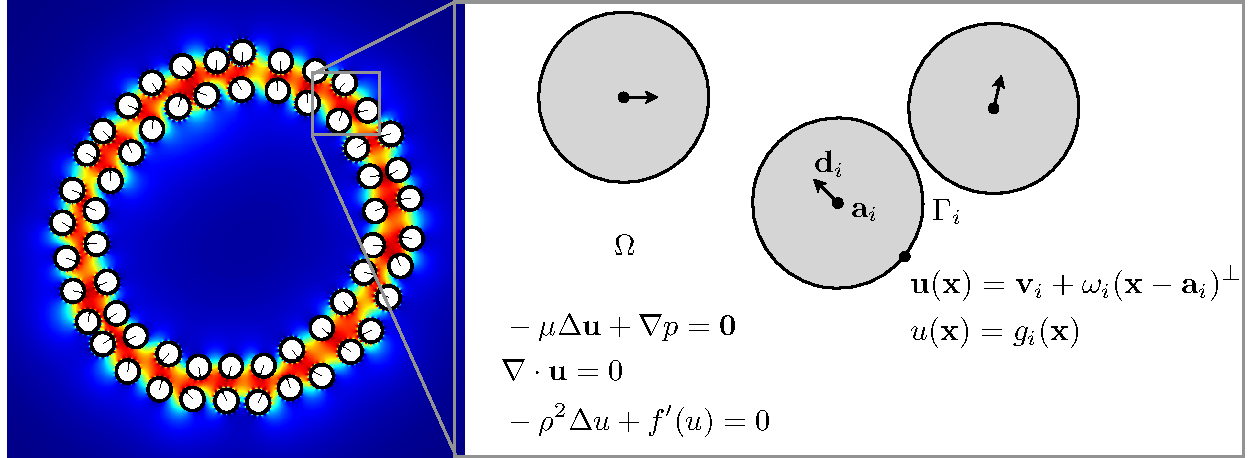
\includegraphics[width=0.55\textwidth]{figures/SpecificAim1/Domain.pdf}
  \caption{\label{fig:flow_map} A collection of amphiphilic particles
  suspended in a solvent. The solvent velocity satisfies the Stokes
  equations, and the hydrophobic forces depend on the solvent activity
  that satisfies the screened Laplace equation. The geometry is updated
  by solving the mobility problem.}
\end{wrapfigure}

The mathematical formulation is a nonlinear system for the dynamics of a
collection of particles. The interactions come from a system of linear
partial differential equations (PDEs) and comprise hydrodynamic
interactions and hydrophobic interactions.
%The formulation prevents particle collisions through excluded volume
%potentials. 
The hydrodynamic interactions come from the mobility problem for rigid
particles immersed in a viscous solvent, which we solve with a
second-order Adams-Bashforth method. Assuming inertial terms are
negligible, the particle motion is goverened by the Stokes equations
\begin{subequations}
  \label{eq:stokes}
  \begin{alignat}{3}
  \label{eq:stokes1}
  -\mu \Delta \uu + \nabla p &= \mathbf{0}, && \xx \in \Omega, \\
    \label{eq:stokes2}
  \nabla\cdot \uu &= 0, \qquad && \xx \in \Omega, \\
\label{eq:stokes3}
  \uu - \uu_\infty &\to \mathbf{0}, && |\xx| \to \infty,
  \end{alignat}
\end{subequations}
%\begin{alignat}{3}
%\label{eq:stokes1}
%  -\mu \Delta \uu + \nabla p &= \mathbf{0}, 
%    && \xx \in \Omega, \\
%\label{eq:stokes2}
%  \nabla\cdot \uu &= 0, \qquad && \xx \in \Omega, \\
%\label{eq:stokes3}
%  \uu - \uu_\infty &\to \mathbf{0}, && |\xx| \to \infty,
%\end{alignat}
%
where $\uu$ is the velocity and $p$ is the pressure of the solvent,
$\uu_\infty$ is the background flow, and $\mu$ is the constant solvent
viscosity. The domain $\Omega$ is the fluid region surrounding the
particles. Since the particles are rigid, the solvent velocity satisfies
a no-slip boundary condition for a rigid body motion 
%\begin{align}
%\label{eq:rigid_bc}
%  \uu(\xx) = \vv_i + \omega_i  (\xx - \aa_i)^\perp, \quad
%    \xx \in \Gamma_i,\qquad  i=1,\ldots,N_p,
%\end{align}
on the particle boundary $\Gamma_i$ with translational velocity $\vv_i$
and angular velocity $\omega_i$. Given imposed forces acting on each
particle, the \emph{mobility problem} consists of finding
translational and angular velocities so that viscous fluid forces
balance the imposed forces.

The hydrophobic interactions come from the tendency of particles to
minimize the free energy of the structure of the surrounding water
molecules. Experimental measurements suggest that the free energy
functional take the form 
\begin{align*}
\label{eq:free_energy}
  F[u] = C \int_{\Omega} \left(\rho |\nabla u|^2 + \rho^{-1} f(u)\right)
  \,d\xx,
\end{align*}
where $u$ is an order parameter for the structure of water, $\rho$ is a
decay length, $C$ is a constant, and $f(u)$ is a potential.
Hydrogen-bond persistence times are on the order of picoseconds
\cite{MaGa13}. Since waters reorient on a time scale much smaller than
the particle motion, $u$ minimizes $F[u]$ at all time, and therefore
satisfies 
\begin{equation}
\label{eq:SL}
-\rho^2 \Delta u + f'(u) = 0  \text{ in } \Omega,\quad u = g,
\text{ on } \bd\Omega.
\end{equation}
The boundary condition $g$ is a material label that is transported with
the particle motions (Figure~\ref{fig:bcs}).

\begin{wrapfigure}[10]{r}{0.65\textwidth}
  \vspace{-22pt}
  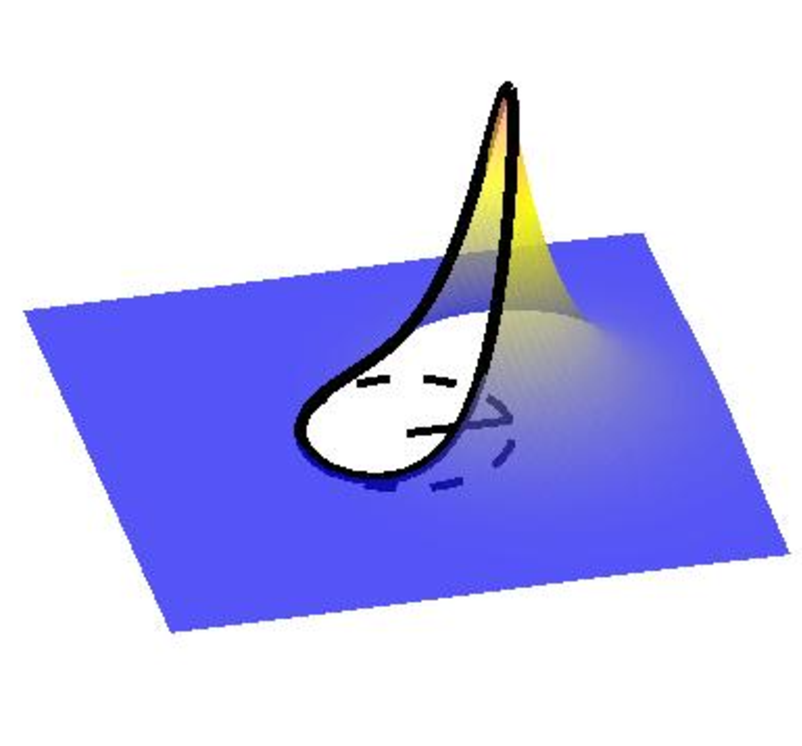
\includegraphics[width=0.2\textwidth]{figures/SpecificAim1/LPA.pdf}
  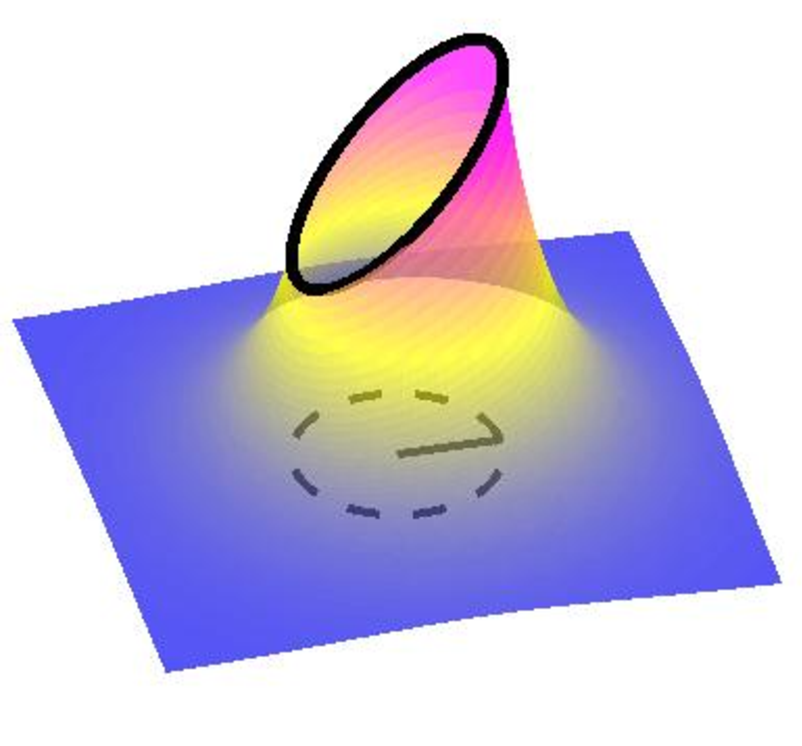
\includegraphics[width=0.2\textwidth]{figures/SpecificAim1/LPB.pdf}
  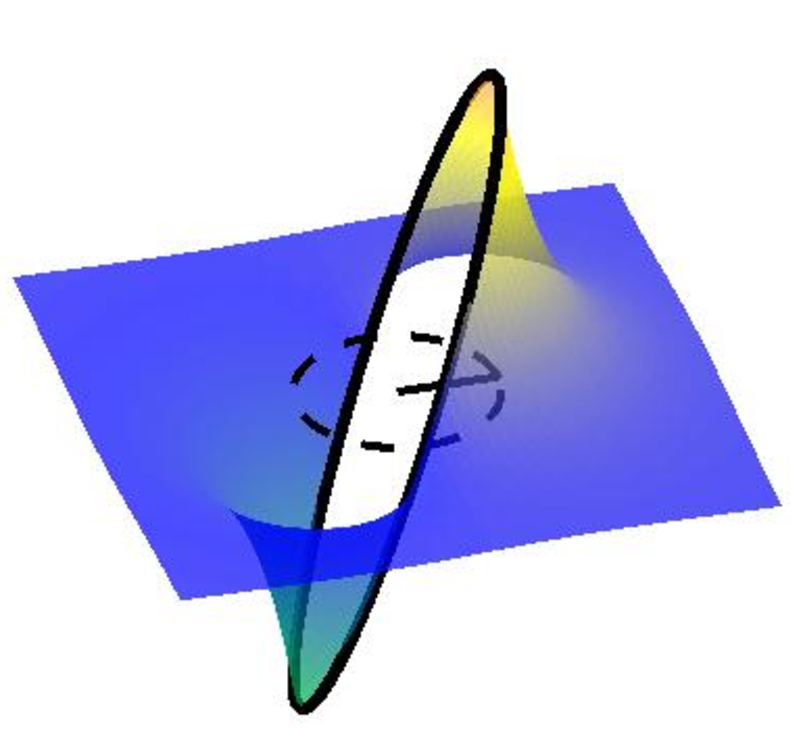
\includegraphics[width=0.2\textwidth]{figures/SpecificAim1/LPC.pdf}  
\caption{\label{fig:bcs} Boundary conditions characterize the type of
  water structure: an amphiphilic particle (left), a hydrophobic
  particle with anisotropic intensity (middle), a water structure with
  plus/minus polarity (right). The dashed curve is the boundary of the
  disk and the arrow its director.}
\end{wrapfigure}
The coupling between the Stokes equations \eqref{eq:stokes} and the
semilinear elliptic equation \eqref{eq:SL} comes from the first
variation of the energy functional. The particles minimize the free
energy $F[u]$ by altering the location of hydrophobic interfaces. It is
possible to calculate the rate of change of $F[u]$ using variation of
the domain~\cite{Bandle2015, Schiffer1954, Grinfeld2010}. Carrying out
this variation yields a 
%The hydrophobic forces are torques are
%\begin{equation}
%  \label{eq:hydrophobicAttraction}
%  \FF_i^{\text{hydro}} = \int_{\Gamma_i} {\bf T}\cdot \nnu \, \dif s, 
%    \quad 
%    T_i^{\text{hydro}} = \int_{\Gamma_i} (\xx - \aa_i)^{\perp} \cdot
%    ({\bf T} \cdot \nnu) \dif s.
%\end{equation}
surface force density 
\begin{align}
  \label{eq:stress}
\mathbf{T}
= C \left[ \rho^{-1} f(u) \mathbf{I}
  + \rho \left(|\nabla u|^2 \mathbf{I} - \nabla u \nabla u^T\right)\right].
\end{align}
The imposed forces and torques from the integration of $\mathbf{T}$
along the particle boundary. The density~\eqref{eq:stress} was first
introduced by~\cite{Fu2018_SIAM} and is the higher-dimensional analogue
of disjoining pressure calculated by \cite{MaRa76, ErLjCl89, KoNa15,
Nagle17, KUZMIN2005}. It is the mathematical ingredient responsible for
forming particle aggregates that sequester their hydrophobic surface
regions.

%By solving the above system, we obtain translational and angular
%velocities of the many-body system. A second-order Adams-Bashforth
%scheme updates the particle positions and orientations.

The formulation presents a number of mathematical and numerical
challenges. For one, the domain is constantly changing so that a new
boundary value problem must be solved at each time step.  The particle
boundaries are nearly touching and this requires high-order numerical
schemes to accurately calculate forces and adaptively chose an
appropriate time step size. Furthermore, there are issues with
accurately capturing the far-field boundary conditions in the unbounded
domain. Finally, the numerical routine must handle large system sizes
efficiently when their are many particles is large. 

%and
%\begin{equation}
%  \label{eq:force}
%  \int_{\Gamma_i} \ssigma \cdot \nnu \, \dif s = \FF_i,\quad 
%  \int_{\Gamma_i} (\xx - \aa_i)^{\perp} \cdot (\ssigma \cdot \nnu) \,
%  \dif s = T_i, \qquad i=1,\ldots,N_b,
%\end{equation}
%where
%$\ssigma = -p \mathbf{I} + \mu \left(\nabla \uu + \nabla \uu^T \right)$
%is the hydrodynamic stress tensor (pressure tensor) and $\nnu$ is the
%particle outward normal.

\subsubsection{Janus-particle self-assembly} 
When $f(u) = u^2$, and the water structure has its lowest potential
value at $u=0$ which represents bulk water. The solutions of
\eqref{eq:SL} have a boundary layer structure and decay to $0$ in the
bulk with the decay length $\rho$. Even in this linear response case, a
number of morphologies arise by altering boundary conditions.

\begin{figure}[h!]
  \begin{center}
    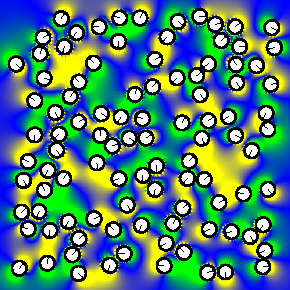
\includegraphics[width=0.32\textwidth]{figures/SpecificAim1/N100A1.pdf}
    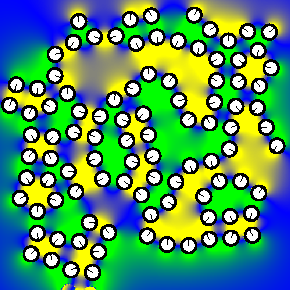
\includegraphics[width=0.32\textwidth]{figures/SpecificAim1/N100A2.pdf}
    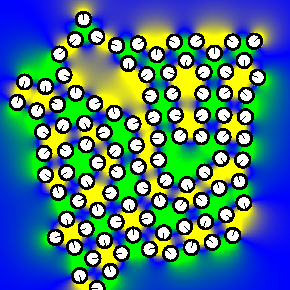
\includegraphics[width=0.32\textwidth]{figures/SpecificAim1/N100A3.pdf}
    \end{center}
  \caption{\label{fig:self-assemblyA} Self-assembly with a polar
  boundary condition leads to a checkerboard pattern. Green is for $u <
  0$, yellow is for $u > 0$, and blue is for $u = 0$.}
\end{figure}

Consider a polar boundary condition where $g_i(\xx) = (\pi r)^{-1/2}
\cos (\theta_i(\xx))$ where $\theta_i$ is the angle formed by $\xx$, the
particle center $\aa_i$, and the particle director $\dd_i$. The
normalization $(\pi r)^{-1/2}$ and others below provide a uniform
surface energy $\int_{\Gamma_i} g_i^2 \,ds = 1$ for circular particles
of radius $r$. The boundary condition is odd along the particle axis
making the particle head repel the tail.  We simulate the dynamics of
100 particles with random initial position and orientation. The
particles rapidly form chains with their directors perpendicular to the
length of the chain. The equilibrium structure consists of particles
positioned on a square grid in a checkerboard pattern
(Figure~\ref{fig:self-assemblyA}. This patterning is a consequence of
energy minimality and allows each particle to simultaneously coordinate
its head with the head of three other particles and its tail with the
tail of three other particles. 

\begin{figure}[h!]
\begin{center}  
    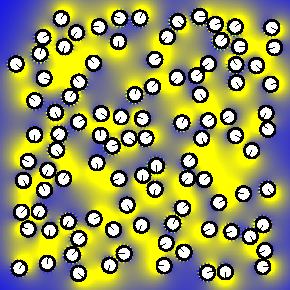
\includegraphics[width=0.32\textwidth]{figures/SpecificAim1/N100B1.pdf}
    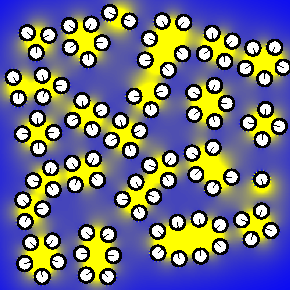
\includegraphics[width=0.32\textwidth]{figures/SpecificAim1/N100B2.pdf}
    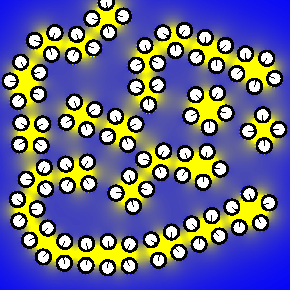
\includegraphics[width=0.32\textwidth]{figures/SpecificAim1/N100B3.pdf}
\end{center}    
  \caption{\label{fig:self-assemblyB} Self-assembly with with boundary
  condition that results in hydrophobic tails and hydrophilic heads. The
  resulting bilayer pattern shields the hydrophobic core (yellow) from
  the aqueous phase.}
\end{figure}
Amphiphilic particles have a hydrophobic tail and a hydrophilic head and
are accounted for as follows. The hydrophilic side takes the value $u =
0$ since the apolar head of a lipid, for example, does not alter
the structure of adjacent waters. The hydrophobic side takes the value
$u > 0$. The interaction between particles is attractive. Using $(3\pi
)^{-1/2}(1 + \cos(\theta_i(\xx)))$ as a simple modification to
the previous boundary condition produces two-dimensional micelles and
bilayers \cite{Fu2018_SIAM} (Figure~\ref{fig:self-assemblyB}).
Researchers have asked us if the phenomenon is robust. To show that it
is, we instead use the boundary condition
\begin{equation}
\label{eq:vonMises}
  g_i(\xx) = \sqrt{
  \frac{\exp( \kappa_i(\theta_i(\xx) - \theta^0_i))}
  {2\pi r_i I_0(\kappa_i)}}
\end{equation}
where the radicand \todo{radicand?} is the von Mises distribution with
director angle $\theta^0_i$ and Bessel function $I_0$ of order zero. The
square of this function behaves as a normal distribution with variance
like $1/\kappa_i$.To replicate experimental conditions, the
concentration $\kappa_i$ and radii $r_i$ are randomized. Using the same
initial configuration, the particles form small groups that
combine to form bilayers (Figure~\ref{fig:self-assemblyC}.


\begin{figure}[h!]
  \begin{center}
    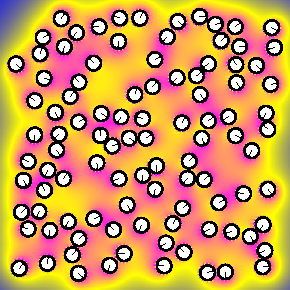
\includegraphics[width=0.32\textwidth]{figures/SpecificAim1/N100C1.pdf}
    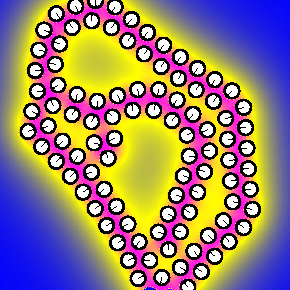
\includegraphics[width=0.32\textwidth]{figures/SpecificAim1/N100C2.pdf}
    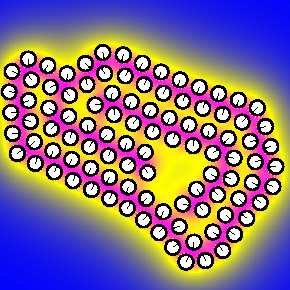
\includegraphics[width=0.32\textwidth]{figures/SpecificAim1/N100C3.pdf}\\
    \caption{Hydrophobic particles with a bias. The hydrophobic
    intensity is greater on one side of the particle (magenta) than the
    other (yellow).
    \label{fig:self-assemblyC}}
\end{center}
\end{figure}

Multilamelar bilayers arise with an increase by shifting the boundary condition
further. Let $g_i(\xx) = (9\pi )^{-1/2}(2 + \cos(\theta_i(\xx)))$.
This gives a hydrophobic particle with greater intensity of hydrophobicity
at $\theta_i = 0$ than at $\theta_i = \pi$.  The initial self-assembly
is similar to that of the amphiphilic particle case, except that the bilayers
do not stay well separated.  Rather, the bilayers stack on top of each
other as a consequence of the interfacial tension of exposed particle heads \cite{deMeetal21}. 

In summary, the hydrophibic interaction-mobility problem model yields
rich morphologies that are valuable in the synthesizing multiphasic and
anisotropic colloids \cite{Bradley2016,Mallory2017,Bradley2017}.
The main experimental challenges include the ability to
decouple particle surface properties.
The goal is to obtain numerically aided 
syntheses and assembly of soft matter materials.
Applications in this area include cargo-carrying capacity, 
catalytic activity, or stimuli-responsive shape-change to amplify colloid
utility for a wide range of  spanning environmental remediation to drug
delivery \cite{McBr21, HaBr20}.







%\begin{wrapfigure}[14]{l}{0.5\textwidth}
%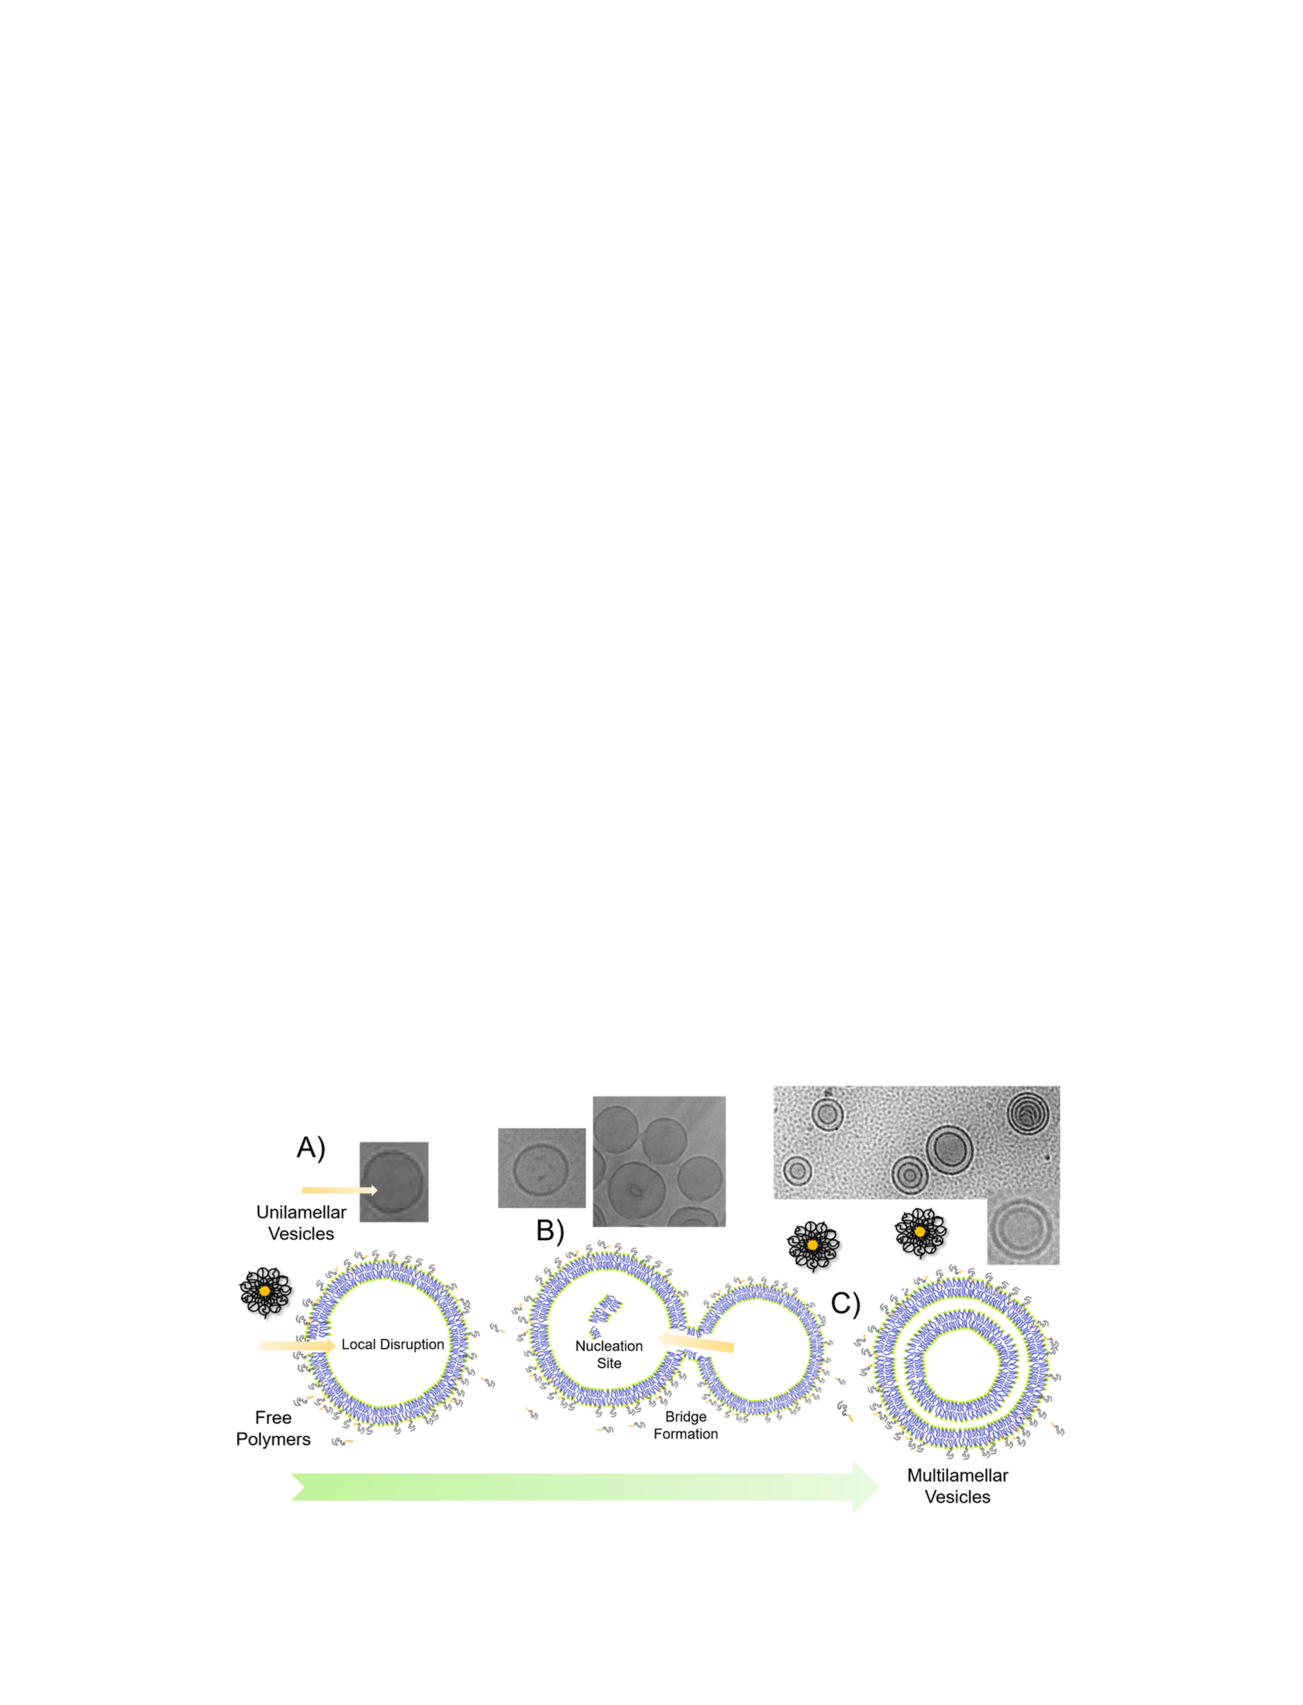
\includegraphics[width=0.5\textwidth]{figures/SpecificAi%m1/multilamelar.pdf}
%\caption{\label{fig:multilamelar}
%  Experimentalists can transform unilamellar vesicles to% multilamellar
%  vesicles by altering the quality of the solvent
%    \cite{deMeetal21}.
%  In \eqref{eq:SL}, the solvent quality enters through t%he potential
%  $f(u)$ and boundary conditions. 
%}
%\end{wrapfigure}
The main modeling challenge is to translate the phenomenological
parameters, e.g. boundary conditions, into measurable quantities
such as contact angles. Collaboration with experimental groups will
use numerical methods to predict parameter regimes 
to control particle-particle interactions. In Specific Aim 3, we
discuss how to include ions and surface charge. 

\subsubsection{Hydrophobic forces as capillary wetting}
A natural generalization of the linear response model is to use a
fourth-order, tilted double-well potential $f(u) = a(u-u_0)^2(u-u_1)^2 +
bu$. Motivated by capillary wetting, soft matter physicist Gerhard
Gompper introduced a double-well model for one-dimensional hydrophobic
attraction \cite{GoHaKo94}. The two-dimensional attraction we propose is
more complicated and includes extra line tension effects not present in
the one-dimensional theories. 

Here, the order parameter $u$ is the mean number of nearest neighbors
per water molecule. The value $u_0 = 4$ gives a local minimum for the
ideal tetrahadral water network found at hydrophobic surfaces. The value
$u_1 \sim 4.4$ gives the absolute minimum in the bulk where there is a
mixture of four and five-coordinated waters. When particles are
well-separated, the energetic cost for filling the interstitial region
with $u_0$-phase water is prohibitive and there is a phase shift from
the $u_0$ to $u_1$ water order---the attraction landscape is more or
less identical to the linear response theory. Conversely, when particles
are proximal, it becomes energetically favorable to coalesce
$u_0$-phases. This introduces a line tension for the phase transition.

Equation~\eqref{eq:SL} takes the form of a steady-state Allen-Cahn
equation. The Allen-Cahn equation is used in phase field formulations of
immisible fluids, for example. PI RR and colaborators launched the
simulation and asymptotic analysis of phase field functionals of
membrane elastic energy, devising functionals for for the squared mean
curvature (Willmore) energy~\cite{0951-7715-18-3-016}, spontaneous
curvature~\cite{Du05} and Gaussian curvature energy~\cite{DuEuler}, as
well as energetic variational approaches to coupling membrane elasticity
to fluids~\cite{QiangDu09}. 

One potential application of the Allen-Cahn-type formulation is to
explaning measured hydrophobic attraction profiles.
The experimental data on hydrophobic attraction between 
is well-established and the literature contains data for a number of
solvents and hydrocarbon species. The experimental measurements
are well-fit by a double exponential curve in the 10 to 100 nanometer range
of separation. Below 10~nm, however, there is an amplification of force
and the attraction follows a much steeper force law not accounted
for by past phenomenoloical theories~\cite{Lin2005}.

It may be the case that the double-well formulation recreates the long
and short-range interactions. The advantage is that the two-dimensional
simulations can replicate the experimental setup better than prior,
one-dimensional theoretical work Some of the model parameters directly
connect to long-range decay lengths and energy cost of creating
hydrophobic-water interfaces with established ranges of values. Other
parameters, like the well structure, are fit to the measured data. These
base-line simulations will allow us to move on to provide more accurate
colloidal suspension simulations. 

Other approaches will be required if the modified phenomenological
theory does not recreate the measured force curves. We can rule out
convection in the water structure since the time scale of particle
motion is much larger than the hydrogen-bond lifetimes. One approach is
to consider Gaussian fluctuation. Here, we expand the free energy
functional around the saddle point solution. The fluctuation energy
then involves calculation of the eigenfunctions of the second variation
of the free energy. This accounts for the fact that experimental
measurements are carried out at finite temperatures, where thermal
fluctuations should ideally also be considered. 

%
% The following commented out Nov 6, 2021.
%
%
\begin{comment}
The goal of Specific Aim 1 is to characterize the material properties of
many-body, self-assembled amphiphiles.  For amphiphiles assembled into
bilayers, these properties are described by membrane continuum
mechanics.  Our goal is to map the parameters of the particle-based
model onto the elastic moduli from continuum theory.  Results from this
goal will facilitate simulators to use the hydrophobic attraction force
calculations to model bilayers with specific composition. These
calculations have provably less computational complexity than those of
molecular dynamics simulations and possess the molecular granularity
lacking from continuum models.

Hamm and Kozlov (HK) pioneered the modern theory of membrane continuum
mechanics~\cite{Hamm2000}, and their theory is widely used to describe
biological phenomena, including fission \cite{FrEsAkSh15, Maetal15,
PhysRevE.79.031926}, fusion \cite{ChKo08,
KoKo2002,Kuzmin7235,Aeffner2012}, poration~\cite{Gaetal20}, phase
boundaries, and interaction with inclusions~\cite{SeLeMaEg17,Saetal20,
Pietal20}. These phenomena require resolution of the internal structure
of the membrane.  Recently, there has been a revival of interest in the
HK theory as the quadratic assumption for the elasticity energy density
has caused researchers to question the applicability of the theory for
large curvatures~\cite{PhysRevLett.117.188102, ARGUDO20161619}.
%
\begin{wrapfigure}[11]{l}{0.47\textwidth}
\centerline{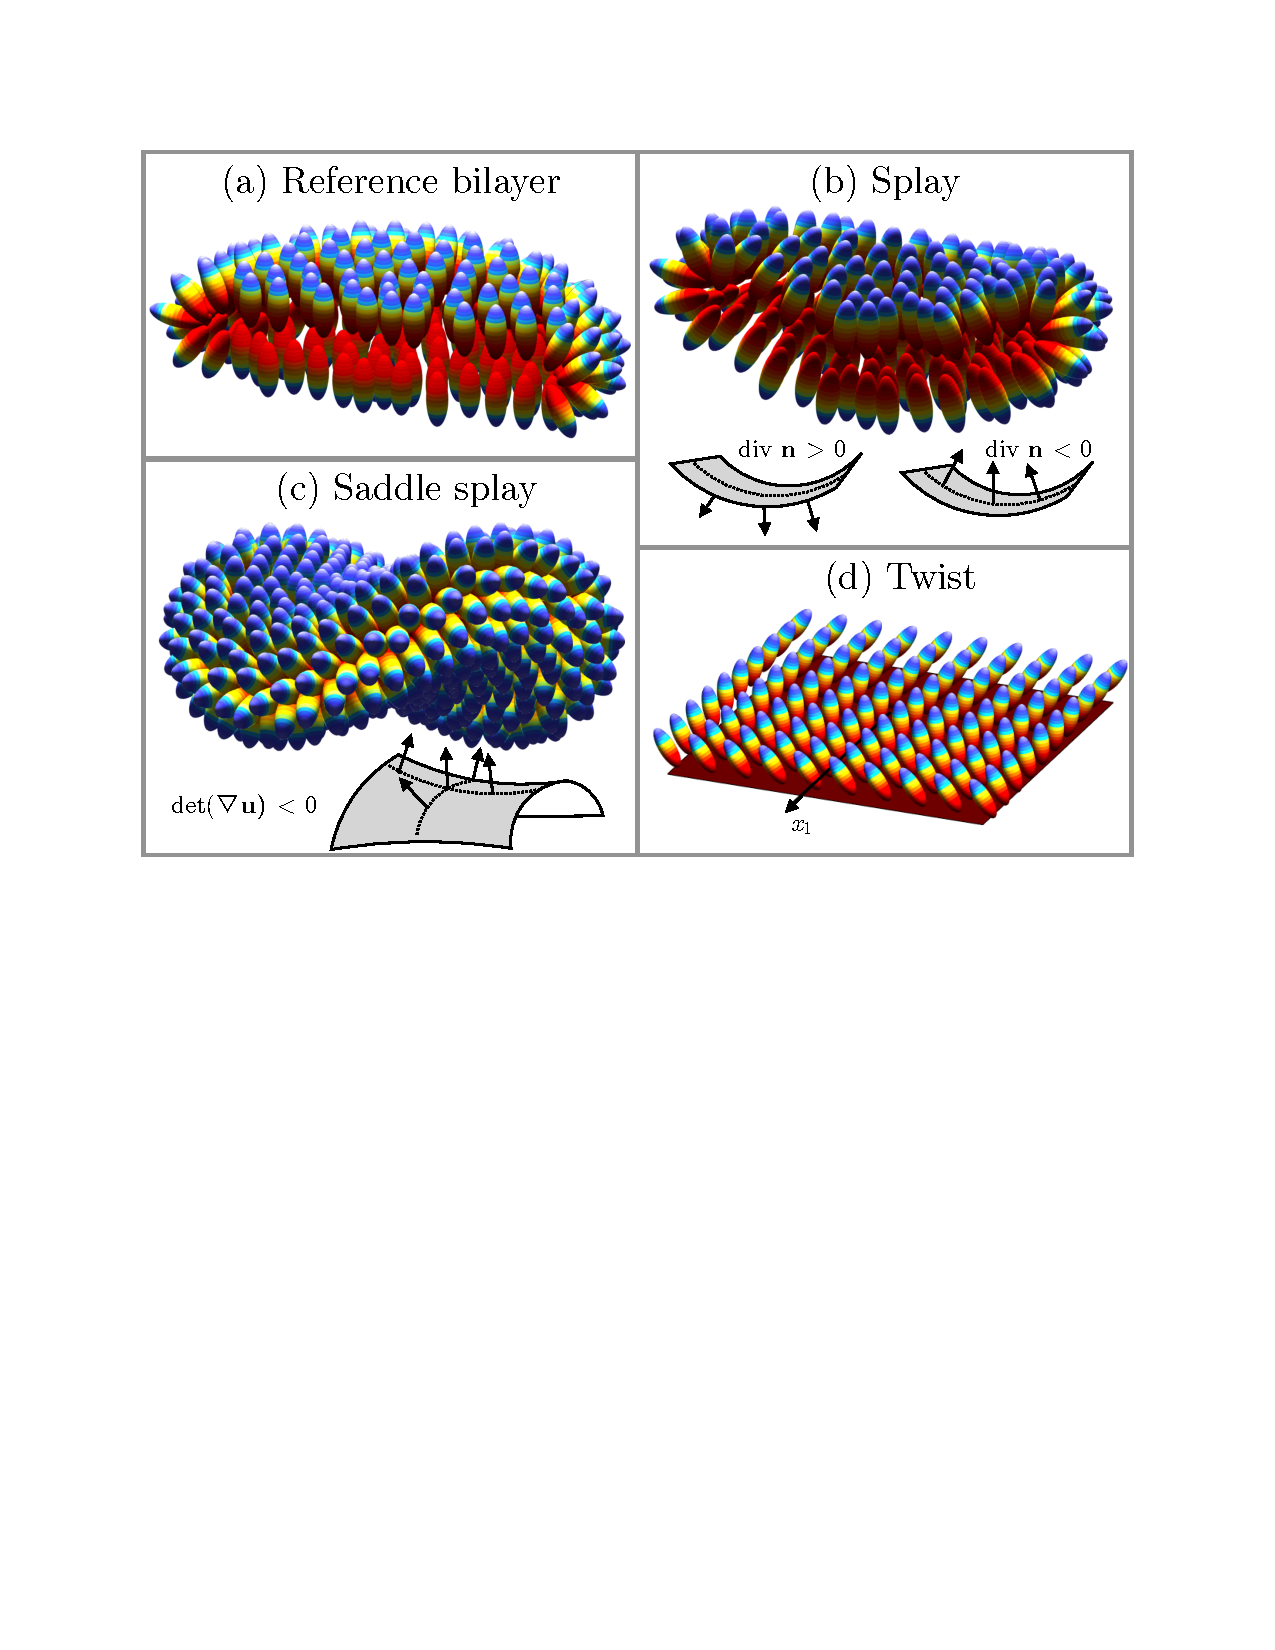
\includegraphics[width=0.46\textwidth]{Figures/Deformations.pdf}}
  \vspace{-5pt}
\caption{\label{fig:deformations} \footnotesize Sketch of the HK
 membrane model \cite{Hamm2000}.}
\end{wrapfigure}
%
This proposal will develop much-needed mathematical analysis to resolve
these controversies due to the assumptions in the HK theory. 


\sloppy
The HK framework assumes a three-dimensional lipid monolayer where the
internal structure consists of straight fibers that represent elongated
hydrocarbon chains.  The elastic energy density ${\cal W}$ is quadratic
in the Green-Lagrange strain tensor for this striated, internal
structure. This energy density decomposes into four, fundamental, and
independent deformations (Figure~\ref{fig:deformations}): splay ($\Div
{\bf n}$), twist ($\Curl {\bf n}$), saddle splay ($\det \nabla {\bf
n}$), and tilt ${\bf t}={\bf n}/({\bf N}\cdot {\bf n}) - {\bf N}$ where
${\bf N}$ is the unit surface normal;
\begin{equation}
\label{ansatz3}
{\cal W} \equiv \int_{\Sigma} 
  \tfrac{1}{2}\KB\left[ \left( \Div {\bf n} + k_0\right)^2 - k_0^2\right] 
+ \tfrac{1}{2}\KT (\Curl {\bf n})^2 + \KG  \det \nabla {\bf n} + \tfrac{1}{2}\KTH |{\bf t}|^2 \,dA.
\end{equation}
Here, the deformations come with elastic coefficients: the bending
modulus $\KB$, twist modulus $\KT$, saddle-splay modulus $\KG$, and tilt
modulus $\KTH$. The parameter $k_0$ is the spontaneous curvature and
determines the preferred lipid splay~\cite{RoLi15,Kozlov2007}.  

Although the HK elastic theory assumes small deformations, Galimzyanov
{\em et al.}~\cite{C9SM02079A} have shown that energies derived from
molecular dynamics and those derived from \eqref{ansatz3} are in
agreement, even when curvatures are large.  Under spatial scales much
larger than the membrane thickness, membrane energy is
well-characterized by the Canham-Helfrich energy used throughout the
fluid-structure literature \cite{QiangDu09, Lowengrub07,KimLai2010_JCP,
Hu, HuLaiSeolEtAl2016_JCP, qua-bir2014, qua-vee-you2019}. The
Canham-Helfrich energy is actually a special case of \eqref{ansatz3}
obtained by setting ${\bf n} =  \pm {\bf N}$ (the $\pm$ depending on
orientation) and collapsing both monolayers onto the membrane midplane.

\subsubsection{Simulations of the HAP model to estimate elastic moduli
and energy}
\begin{wrapfigure}[11]{r}{0.43\textwidth}
  \centerline{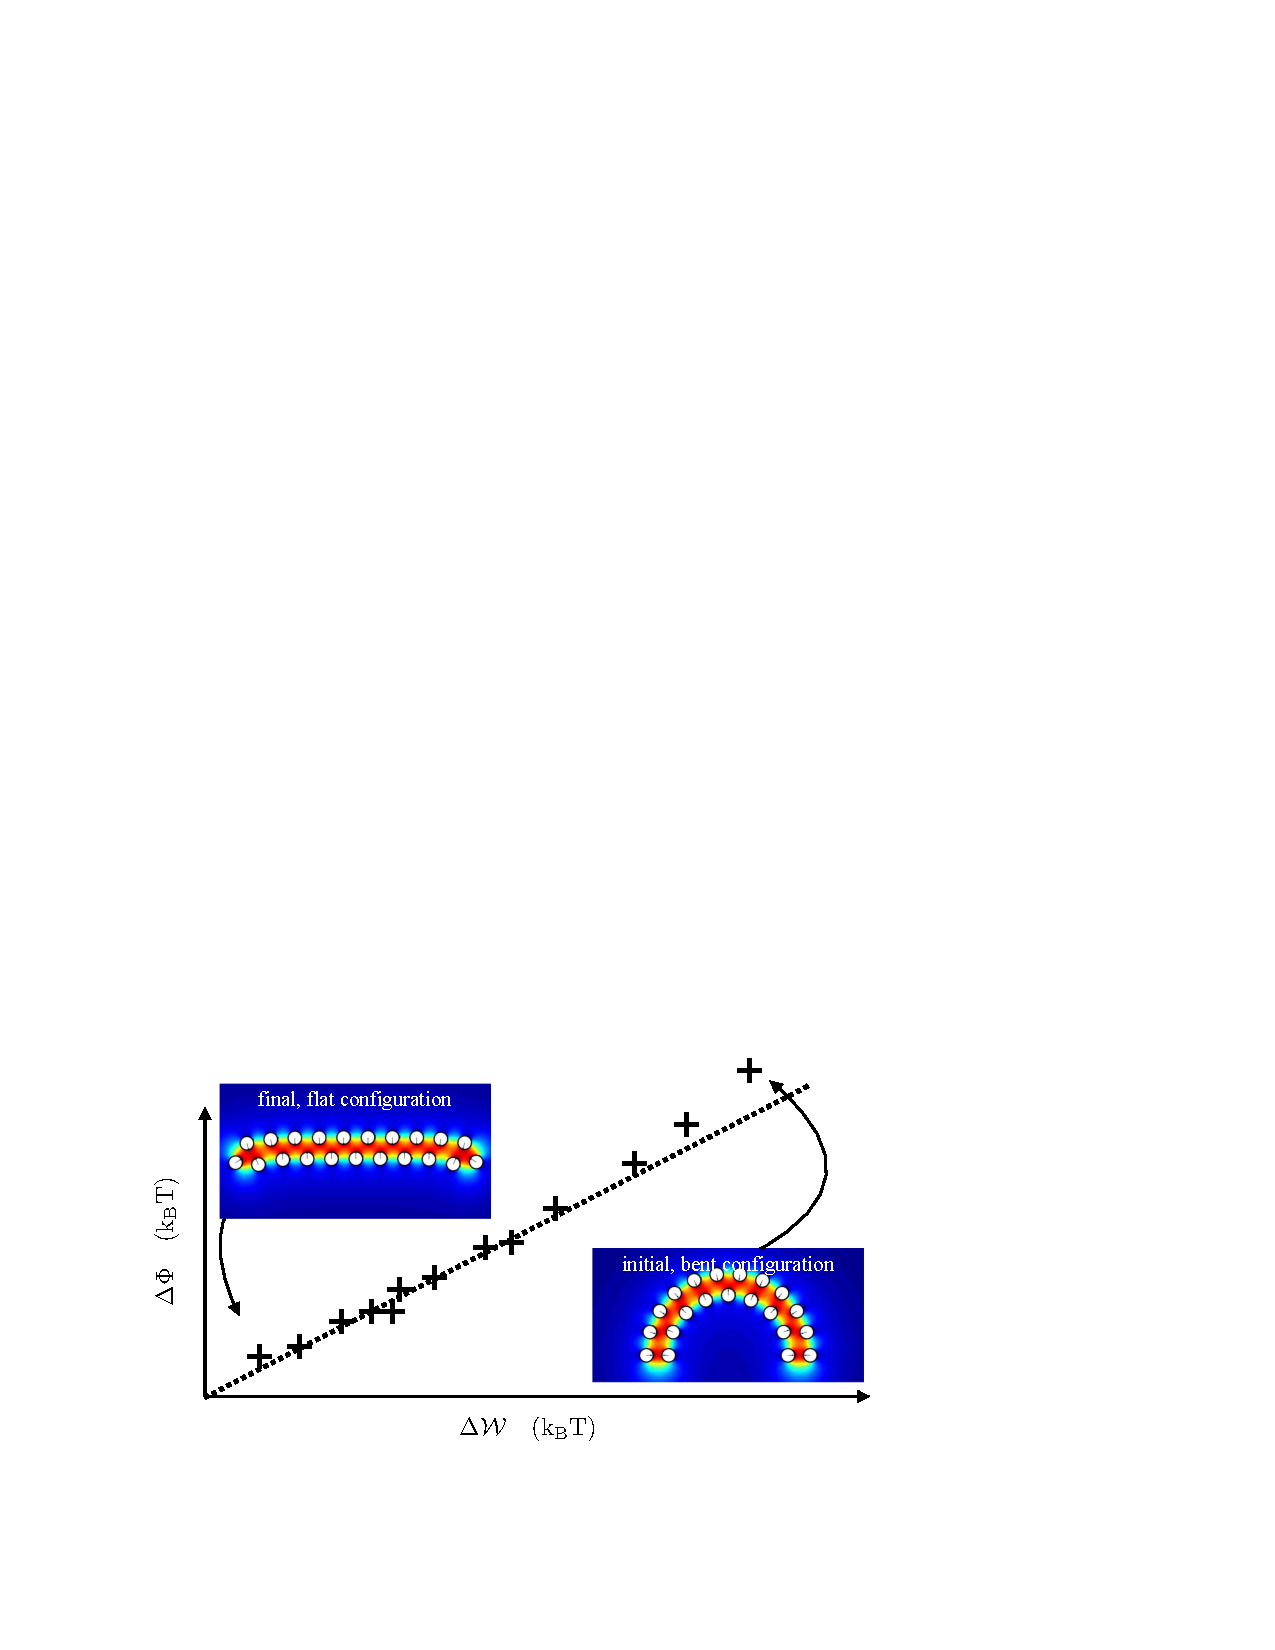
\includegraphics[width=0.42\textwidth]{Figures/Flattening.pdf}}
  \caption{\label{fig:flattening} \footnotesize Example of computing
  bending modulus of a lipid bilayer from particle simulation.}
\end{wrapfigure}
We propose to {\bf (i)} determine the value of effective elastic moduli
$\KB$, $\KT$, $\KG$, and $\KTH$ and then {\bf (ii)} understand how the
model parameters $\rho,$ $\gamma$, and the particle shape map onto
elastic moduli. An accurate and robust way to measure material
properties is to track the evolution of the bilayer as it relaxes from
an initially non-equilibrium
configuration~\cite{PhysRevLett.117.188102}.
Figure~\ref{fig:flattening} shows an example where the initial
configuration of a bilayer patch containing the splay deformation
without any other components (saddle splay, twist and tilt). As the bent
membrane flattens, both the self-interaction energy $\Phi$ and the
elastic energy ${\cal W}$ decrease, and because the saddle splay, twist,
and tilt stay zero, the slope gives the bending modulus in this case. 

Here we start with a particle-based bilayer in a specific
non-equilibrium shape that involves only one of the components of the
displacement in Figure~\ref{fig:deformations}, and then evolve the
particle system according to the time integration for \eqref{eq:stokes}.
Because elastic properties are independent of dissipation, we can forgo
solving for fluid velocity and set the translational velocity and
angular velocity directly proportional to the force and torque,
respectively. 

This yields a dissipation of the total potential \eqref{eq:total_poten},
which stabilizes the evolving bilayer shape. Therefore, we reconstruct
an evolving monolayer dividing surface $\Sigma$ and director field ${\bf
n}$ by interpolating the particle centers and orientations.
Using~\eqref{ansatz3}, we calculate a continuum energy $\mathcal{W}$
from the interpolated shapes.

We propose to conduct calculations similar to the example of
Figure~\ref{fig:flattening} for other elastic moduli such as the
effective twist modulus $\KT$.  Molecular dynamics investigations find a
twist modulus about 1 \kBT~\cite{LeVeWa14}, and here, the specific
non-equilibrium shape consists of a single layer of amphiphilic
particles on a hydrophobic substrate as illustrated by
Figure~\ref{fig:deformations}D. Having a nonzero twist requires nonzero
tilt because the surface gradient of the lipid director equals the
second fundamental form whenever tilt is zero locally. The twist
deformation is a fully three-dimensional deformation.
\S\ref{subsec:specific_aim_3} addresses outstanding implementation
issues like three-dimensional boundary integral equation solvers.

The gradient descent technique is ineffective for measuring the saddle
splay modulus $\KG$ because the saddle splay energy is largely invariant
under shape changes.  To evaluate $\KG$, we will combine the present
particle simulations with the string method from PI RR's work on
membrane fusion \cite{RyKlYaCo16}. The string method is a numerical
scheme that finds least energy pathways separating energy basins
\cite{doi:10.1063/1.2720838}.  In the simplified Canham-Helfrich
formulation, saddle splay energy is an exact indicator of topological
transitions, thanks to the  Gauss-Bonnet theorem \cite{TerziDeserno17}.
More generally, PI RR has shown that saddle splay acts as a topological
indicator even in the presence of nonzero tilt \cite{RyKlYaCo16}.  As a
result, saddle splay can be quantified from the transition energies of a
least energy path of pore formation (Figure~\ref{fig:saddle_splay}).

The field of membrane continuum mechanics still lacks consensus as to
whether HK energy is the appropriate functional for bilayer energy.
\textbf{(i)} Researchers have assumed that $\KT = 0$ to effect lateral
fluidity in membranes~\cite{Hamm2000, TerziDeserno17, C9SM02079A,
PhysRevE.102.042406}. A value $\KT = 0$, however, makes~\eqref{ansatz3}
a noncoercive functional. \textbf{(ii)} Recently,~\cite{TerziDeserno17}
derived a tilt curvature term that was neglected from the HK
analysis~\cite{Hamm2000}.  Later,~\cite{C9SM02079A}
and~\cite{PhysRevE.102.042406} independently identified an inconsistency
in the argument used by~\cite{TerziDeserno17} arising from a transversal
tilt invariance assumption.  In~\cite{RyKlYaCo16}, PI RR and
collaborators showed that the tilt vector leads to unphysical cusps
depending on how one accounts for membrane thickness.  \textbf{(iii)}
Theoretical analysis of lipid phase transitions predict a negative
saddle-splay modulus around $-8$ \kBT~\cite{SIEGEL2004366,
SIEGEL20085200} that gives rise to a larger energy barrier for monolayer
fusion than is found by experiments~\cite{FrRoPi17, Tran7106,
TerziDeserno17}.
\begin{wrapfigure}[11]{l}{0.32\textwidth}
  \centerline{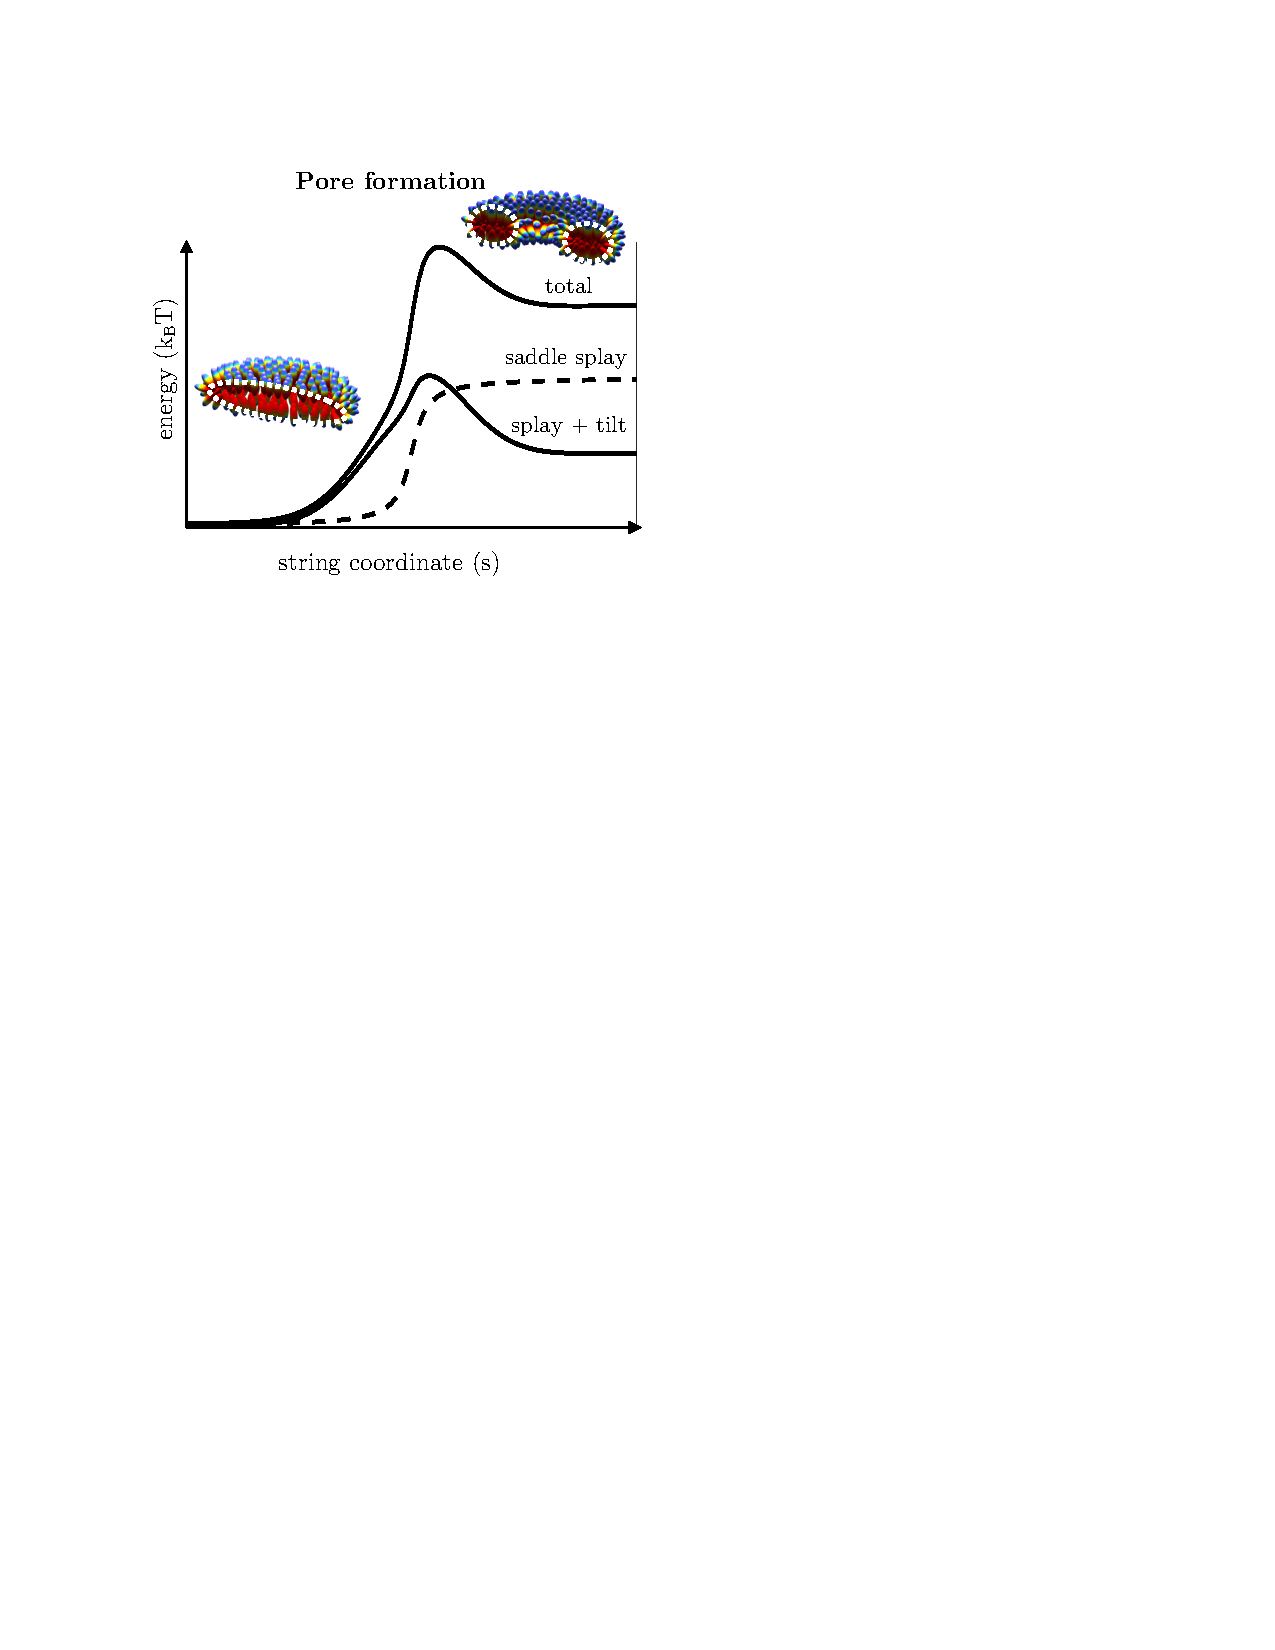
\includegraphics[width=0.31\textwidth]{Figures/SaddleSplayDiagram.pdf}}
  \caption{\label{fig:saddle_splay} \footnotesize Example of determining
  the saddle splay modulus.}
\end{wrapfigure}

The form of the elastic energy density~\eqref{ansatz3} is the same as
the Oseen-Frank energy density for nematic liquid
crystals~\cite{ANDRIENKO2018520, Tran7106, Helfrich73}. In fact, a lipid
monolayer acts as one layer in a smectic phase~\cite{REYESMATEO1995978,
Rangamani20140463, PhysRevLett.113.248102}. Based on this observation,
we propose to examine the HK analysis to resolve the aforementioned
inconsistencies. We will expand the strain tensor in terms of a plane
perpendicular to ${\bf n}$ (instead of the monolayer tangent plane as
done in the past works) so that the gradient terms in the elastic energy
completely decouple. Using this expansion we prove an exact identity
that gives the incompressibility condition by a Steiner-type polynomial
in $\Div {\bf n}$ and $\det \nabla {\bf n}$ \cite{Fe59}. In contrast,
the works~\cite{TerziDeserno17, PhysRevE.102.042406, Hamm2000,
C9SM02079A} utilize an approximate identity for incompressibility as a
base, so we can considerably improve upon the analysis of monolayer
energy.

\subsubsection{Analysis of the HAP model in terms of the HK functional}
The HK functional~\eqref{ansatz3} has transformed how scientists understand biological membranes, yet the
theory has received little attention in terms of
mathematical analysis. In the calculus of variations, the
principal question is whether a minimizer of an energy functional
exists. In the case of~\eqref{ansatz3}, the answer is presently unknown.
With regard to the simpler Canham-Helfrich energy,~\cite{Simon1993}
proved the existence of minimizing surfaces without boundary,
and~\cite{doi:10.1137/18M1195851} proved the well-posedness of a
spatially periodic, time-dependent elastic interface problem. An
analytical challenge for the HK functional~\eqref{ansatz3} is that
surface-director coupling makes it possible to have bounded energy
monolayers with corners, and such pathological examples must be ruled
out before carrying over the arguments for the Canham-Helfrich
functional to the present setting.

Our goal here is to develop tools that can explain functionals
like~\eqref{ansatz3} from first principles in terms of HAP. The
papers~\cite{doi:10.1063/5.0009734, Seguin2012, Seguin2014} give
statistical mechanical/mean field derivations of the Canham-Helfrich
energy from a pair-potential for rod-like molecules, but do not include
tilt, which is an indispensable deformation at biological scales. To
make progress, we must first understand how the HAP functional behaves
under various limits.

We first consider HAP in the limit of vanishing screening length. As a
concrete model problem, we consider a collection of colloidal polyhedral
where the binding energy of this system can be described by a discrete,
lower semicontinuous functional $\Phi_0$ whose value is the total
surface area of the polyhedra minus two times the area of any
overlapping faces. We conjecture that the $\Phi$ energy
$\Gamma$-converges to $\Phi_0$ \cite{Mugnai2013}, meaning that any
cluster points of minimizers of $\Phi$ converge to a minimum of $\Phi_0$
in the limit $\rho \to 0$. To address this conjecture, we employ
boundary layer analysis for the screened Laplace equation~\cite{Lee2018,
Lin2015, Shibata2004,1531-3492_2006_2_357, Lee2018}. The technique of
$\Gamma$-convergence is a powerful tool for numerical approximations and
with it we can help explain unexpected phenomena like hierarchical
self-assembly in colloidal systems~\cite{Luo2019}.

\end{comment}


\subsection{Specific Aim 2: Efficient, high-order methods for
large-scale simulations}
% ----------------------------------------------------------------------
Over the past decade, there has been an explosion of interest in
small-scale processes that utilize capillary forces and van der Waals
interactions to coordinate movement and bind microscopic components in
solvent~\cite{Pandey2011, Zhang2017, Siontorou2017}. Additionally,
hydrodynamic interactions are central to fabricate complex,
three-dimensional microstructures~\cite{Dasgupta2017, Leong2007,
Reynolds2019, Cho2010}. Hydrodynamic effects cannot be ignored since
they, like for the rates of biological functions like pore
dynamics~\cite{RYHAM20112929}, set the rate of dissipation. In Specific
Aim 2, we propose novel and efficient high-order numerical methods to
simulate dynamic assembly of particles under HAP potential in a viscous
solvent. As described in~\eqref{eq:stokes1}--\eqref{eq:stokes3} and
illustrated in Figure~\ref{fig:flow_map}, the solvent phase is modeled
by the Stokes equations for an incompressible, viscous fluid, and these
equations are coupled to the screened-Laplace equation~\eqref{eq:SL}
through viscous and hydrophobic stress balance. 
 
%\label{subsec:specific_aim_2}
%\begin{wrapfigure}[14]{r}{0.61\textwidth}
%  \centering{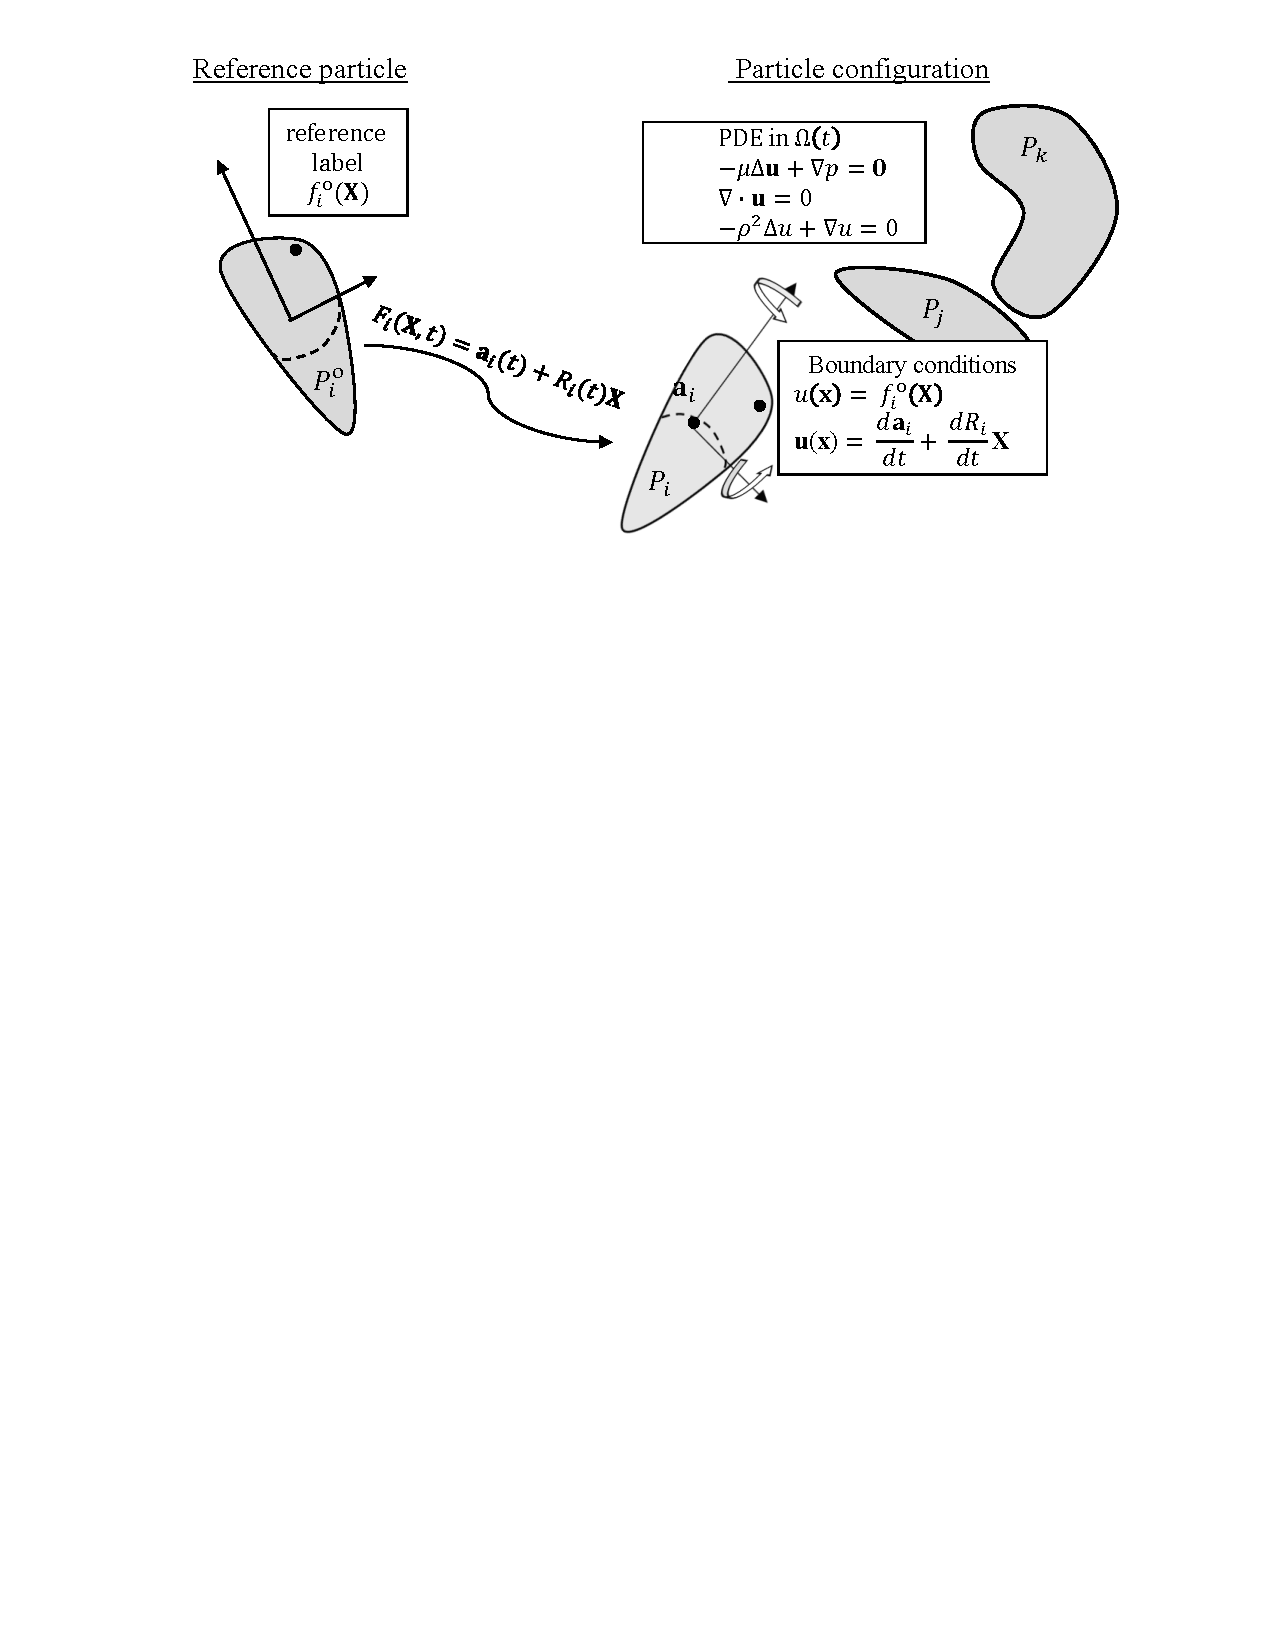
\includegraphics[width=0.60\textwidth]{Figures/domain.pdf}}
%    \vspace{-15pt}
%    \caption{\label{fig:flow_map} \footnotesize A collection of 3D
%    amphiphilic particles suspended in a solvent. The solvent velocity
%    satisfies the Stokes equations, and the hydrophobic forces depend on
%    the solvent activity that satisfies the screened Laplace equation.
%    The geometry is updated by solving the mobility problem.} 
%\end{wrapfigure}
The HAP model requires solving exterior problems for the order
parameter~\eqref{eq:SL} and the Stokes
equations~\eqref{eq:stokes1}--\eqref{eq:stokes3}. We will develop
methods based on combinations of volume and layer potentials. Numerical
methods to solve these integral equations (IEs) have several advantages
over their PDE-based counterpart: by construction, they satisfy
far-field and mass conservation conditions; only $\partial\Omega$ needs
to be discretized for layer potentials; carefully chosen IEs result in a
well-conditioned linear system that is solved with a mesh-independent
number of GMRES iterations; and high-order or spectral accuracy is
attainable with appropriate quadrature methods. The PIs have
demonstrated that IEs are a powerful tool to simulate two-dimensional
suspensions of amphiphilic particles~\cite{Fu2018_SIAM, FuQuRyYo20}.
Moreover, elements of these formulations have been described in three
dimensions~\cite{ying_2006, manasthesis, rac-gre2016}. This proposal
will extend the two-dimensional methods to more general amphiphilic
particle models that satisfy~\eqref{eq:SL}, and all the methods can
naturally be extended to three dimensions. \S\ref{subsec:AC} describes
how the non-linear Allen-Cahn equation~\eqref{eq:SL} will be iteratively
solved using BIE formulations. Then, \S\ref{subsec:NumericalIssues}
describes how we will combine preconditioning strategies with fast
summation methods to accelerate the time to solution, and
\S\ref{subsec:timeStepping} describes adaptive time stepping methods,

\subsubsection{Iterative methods for the Allen-Cahn HAP model}
\label{subsec:AC}

The PIs have developed numerical methods to solve~\eqref{eq:SL} when
$f(u) = u^2$---this choice results in the linear screened Laplace
equation. For a more general $f$, such as a double well potential, we
will interpret the solution of~\eqref{eq:SL} as the root finding problem
\begin{align}
  \label{eq:F}
  J[u] = -\rho^2 \Delta u + f'(u).
\end{align}
This non-linear PDE will be solved with Newton's method
\begin{align*}
  u^{N+1} = u^{N} - \alpha (dJ^N)^{-1} J(u^N),
\end{align*}
where $dJ^N = -\rho^2 \Delta + f''(u^N)$ is the Fr\'{e}chet derivative
of $F$, and $\alpha$ is the step size which will be determined using
backtracking. As expected, the biggest computational challenge is
solving $- \rho^2 \Delta v + f''(u^{N}) v = J[u^N]$. Solving this
variable coefficient PDE with an integral equation is challenging since
a fundamental solution is not readily available. We propose to instead
use an inexact Newton's method where $dJ^{-1}$ is defined in terms of
the piecewise quadratic approximation
\begin{align*}
  f(u) \approx \tilde{f}(u) = bu + \begin{cases}
    a(u - u_0)^2, &\mbox{if } u \leq (u_0 + u_1)/2, \\
    (u - u_1)^2, &\mbox{if } u > (u_0 + u_1)/2.
  \end{cases}
\end{align*}
and the resulting inexact Newton's method requires solving the piecewise
constant PDE
\begin{align}
  \label{eq:screenedPoisson}
  -\rho^2 \Delta v + \tilde{f}''(u^{N})v = J[u^N],
\end{align}
which is a screened Poisson equation with piecewise a constant screening
coefficient. We test the efficacy of exact and inexact Newton's method
applied to~\eqref{eq:F} in $(0,1)$ by discretizing $dJ$ with a
second-order finite difference method. The choice of parameters $a$,
$b$, $U_0$, and $U_1$ result in the double well potential illustrated in
Figure~\ref{fig:CA}(a), and both the exact and inexact Newton's methods
converge to the solution in Figure~\ref{fig:CA}(b).
Figure~\ref{fig:CA}(c) shows the max norm of the residual at each Newton
iterate when using the exact second derivative (red curve) and the
piecewise constant approximate (blue curve). While the inexact Newton's
method requires roughly twice as many iterations to reach of a tolerance
of $10^{-4}$, each iteration is significantly cheaper in higher
dimensions.

\begin{wrapfigure}[28]{l}{1.8in}
  \vspace{-4pt}
  \centering
  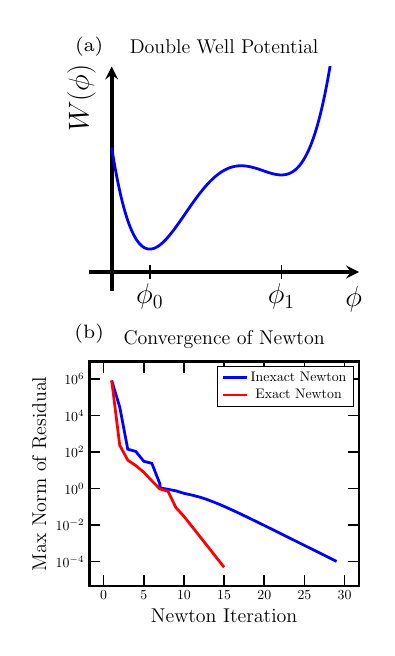
\begin{tikzpicture}[scale=0.5]

\begin{axis}[
  at = {(0cm,0cm)},
  axis line style = {line width=3pt},
  axis lines=middle,
  enlargelimits = true,
  x label style={at={(axis description cs:0.98,0.04)},anchor=north},
  xlabel = {\huge $\phi$},
  y label style={at={(axis description
  cs:-0.10,0.86)},anchor=north,rotate=90},
  ylabel = {\huge $W(\phi)$},
  every major tick/.append style={very thick, major tick length=10pt, black},
  xtick = {4.2292e-01,1.8869e+00},
  xticklabels = {\huge $\phi_0$,\huge $\phi_1$},
  ytick = \empty,
  xmin = 0,
  xmax = 2.5,
  ymin = 0,
  ymax = 1.5,
  title = {\Large Double Well Potential}
]

\addplot[blue,line width=2.0pt] coordinates{
(0.0000e+00,1.0000e+00)
(2.5025e-03,9.8854e-01)
(5.0050e-03,9.7718e-01)
(7.5075e-03,9.6593e-01)
(1.0010e-02,9.5478e-01)
(1.2513e-02,9.4372e-01)
(1.5015e-02,9.3277e-01)
(1.7518e-02,9.2192e-01)
(2.0020e-02,9.1117e-01)
(2.2523e-02,9.0052e-01)
(2.5025e-02,8.8997e-01)
(2.7528e-02,8.7952e-01)
(3.0030e-02,8.6917e-01)
(3.2533e-02,8.5891e-01)
(3.5035e-02,8.4875e-01)
(3.7538e-02,8.3869e-01)
(4.0040e-02,8.2872e-01)
(4.2543e-02,8.1885e-01)
(4.5045e-02,8.0908e-01)
(4.7548e-02,7.9940e-01)
(5.0050e-02,7.8982e-01)
(5.2553e-02,7.8032e-01)
(5.5055e-02,7.7093e-01)
(5.7558e-02,7.6162e-01)
(6.0060e-02,7.5241e-01)
(6.2563e-02,7.4329e-01)
(6.5065e-02,7.3427e-01)
(6.7568e-02,7.2533e-01)
(7.0070e-02,7.1649e-01)
(7.2573e-02,7.0773e-01)
(7.5075e-02,6.9907e-01)
(7.7578e-02,6.9050e-01)
(8.0080e-02,6.8201e-01)
(8.2583e-02,6.7361e-01)
(8.5085e-02,6.6531e-01)
(8.7588e-02,6.5709e-01)
(9.0090e-02,6.4895e-01)
(9.2593e-02,6.4091e-01)
(9.5095e-02,6.3295e-01)
(9.7598e-02,6.2508e-01)
(1.0010e-01,6.1729e-01)
(1.0260e-01,6.0959e-01)
(1.0511e-01,6.0197e-01)
(1.0761e-01,5.9444e-01)
(1.1011e-01,5.8699e-01)
(1.1261e-01,5.7963e-01)
(1.1512e-01,5.7234e-01)
(1.1762e-01,5.6514e-01)
(1.2012e-01,5.5803e-01)
(1.2262e-01,5.5099e-01)
(1.2513e-01,5.4404e-01)
(1.2763e-01,5.3717e-01)
(1.3013e-01,5.3037e-01)
(1.3263e-01,5.2366e-01)
(1.3514e-01,5.1703e-01)
(1.3764e-01,5.1048e-01)
(1.4014e-01,5.0400e-01)
(1.4264e-01,4.9761e-01)
(1.4515e-01,4.9129e-01)
(1.4765e-01,4.8505e-01)
(1.5015e-01,4.7889e-01)
(1.5265e-01,4.7280e-01)
(1.5516e-01,4.6679e-01)
(1.5766e-01,4.6086e-01)
(1.6016e-01,4.5500e-01)
(1.6266e-01,4.4922e-01)
(1.6517e-01,4.4351e-01)
(1.6767e-01,4.3788e-01)
(1.7017e-01,4.3232e-01)
(1.7267e-01,4.2683e-01)
(1.7518e-01,4.2142e-01)
(1.7768e-01,4.1608e-01)
(1.8018e-01,4.1081e-01)
(1.8268e-01,4.0562e-01)
(1.8519e-01,4.0049e-01)
(1.8769e-01,3.9544e-01)
(1.9019e-01,3.9046e-01)
(1.9269e-01,3.8554e-01)
(1.9520e-01,3.8070e-01)
(1.9770e-01,3.7593e-01)
(2.0020e-01,3.7123e-01)
(2.0270e-01,3.6659e-01)
(2.0521e-01,3.6202e-01)
(2.0771e-01,3.5753e-01)
(2.1021e-01,3.5310e-01)
(2.1271e-01,3.4873e-01)
(2.1522e-01,3.4443e-01)
(2.1772e-01,3.4020e-01)
(2.2022e-01,3.3604e-01)
(2.2272e-01,3.3194e-01)
(2.2523e-01,3.2791e-01)
(2.2773e-01,3.2394e-01)
(2.3023e-01,3.2003e-01)
(2.3273e-01,3.1619e-01)
(2.3524e-01,3.1241e-01)
(2.3774e-01,3.0870e-01)
(2.4024e-01,3.0505e-01)
(2.4274e-01,3.0146e-01)
(2.4525e-01,2.9794e-01)
(2.4775e-01,2.9447e-01)
(2.5025e-01,2.9107e-01)
(2.5275e-01,2.8773e-01)
(2.5526e-01,2.8445e-01)
(2.5776e-01,2.8122e-01)
(2.6026e-01,2.7806e-01)
(2.6276e-01,2.7496e-01)
(2.6527e-01,2.7192e-01)
(2.6777e-01,2.6894e-01)
(2.7027e-01,2.6601e-01)
(2.7277e-01,2.6314e-01)
(2.7528e-01,2.6033e-01)
(2.7778e-01,2.5758e-01)
(2.8028e-01,2.5489e-01)
(2.8278e-01,2.5225e-01)
(2.8529e-01,2.4967e-01)
(2.8779e-01,2.4714e-01)
(2.9029e-01,2.4467e-01)
(2.9279e-01,2.4225e-01)
(2.9530e-01,2.3989e-01)
(2.9780e-01,2.3759e-01)
(3.0030e-01,2.3533e-01)
(3.0280e-01,2.3313e-01)
(3.0531e-01,2.3099e-01)
(3.0781e-01,2.2890e-01)
(3.1031e-01,2.2686e-01)
(3.1281e-01,2.2487e-01)
(3.1532e-01,2.2293e-01)
(3.1782e-01,2.2105e-01)
(3.2032e-01,2.1921e-01)
(3.2282e-01,2.1743e-01)
(3.2533e-01,2.1570e-01)
(3.2783e-01,2.1402e-01)
(3.3033e-01,2.1239e-01)
(3.3283e-01,2.1080e-01)
(3.3534e-01,2.0927e-01)
(3.3784e-01,2.0779e-01)
(3.4034e-01,2.0635e-01)
(3.4284e-01,2.0496e-01)
(3.4535e-01,2.0362e-01)
(3.4785e-01,2.0233e-01)
(3.5035e-01,2.0108e-01)
(3.5285e-01,1.9989e-01)
(3.5536e-01,1.9873e-01)
(3.5786e-01,1.9763e-01)
(3.6036e-01,1.9657e-01)
(3.6286e-01,1.9555e-01)
(3.6537e-01,1.9458e-01)
(3.6787e-01,1.9366e-01)
(3.7037e-01,1.9277e-01)
(3.7287e-01,1.9194e-01)
(3.7538e-01,1.9114e-01)
(3.7788e-01,1.9039e-01)
(3.8038e-01,1.8969e-01)
(3.8288e-01,1.8902e-01)
(3.8539e-01,1.8840e-01)
(3.8789e-01,1.8782e-01)
(3.9039e-01,1.8728e-01)
(3.9289e-01,1.8679e-01)
(3.9540e-01,1.8633e-01)
(3.9790e-01,1.8592e-01)
(4.0040e-01,1.8554e-01)
(4.0290e-01,1.8521e-01)
(4.0541e-01,1.8491e-01)
(4.0791e-01,1.8466e-01)
(4.1041e-01,1.8444e-01)
(4.1291e-01,1.8427e-01)
(4.1542e-01,1.8413e-01)
(4.1792e-01,1.8403e-01)
(4.2042e-01,1.8397e-01)
(4.2292e-01,1.8395e-01)
(4.2543e-01,1.8396e-01)
(4.2793e-01,1.8401e-01)
(4.3043e-01,1.8410e-01)
(4.3293e-01,1.8422e-01)
(4.3544e-01,1.8438e-01)
(4.3794e-01,1.8457e-01)
(4.4044e-01,1.8480e-01)
(4.4294e-01,1.8507e-01)
(4.4545e-01,1.8537e-01)
(4.4795e-01,1.8571e-01)
(4.5045e-01,1.8608e-01)
(4.5295e-01,1.8648e-01)
(4.5546e-01,1.8692e-01)
(4.5796e-01,1.8739e-01)
(4.6046e-01,1.8789e-01)
(4.6296e-01,1.8843e-01)
(4.6547e-01,1.8899e-01)
(4.6797e-01,1.8960e-01)
(4.7047e-01,1.9023e-01)
(4.7297e-01,1.9089e-01)
(4.7548e-01,1.9159e-01)
(4.7798e-01,1.9231e-01)
(4.8048e-01,1.9307e-01)
(4.8298e-01,1.9386e-01)
(4.8549e-01,1.9468e-01)
(4.8799e-01,1.9553e-01)
(4.9049e-01,1.9640e-01)
(4.9299e-01,1.9731e-01)
(4.9550e-01,1.9824e-01)
(4.9800e-01,1.9921e-01)
(5.0050e-01,2.0020e-01)
(5.0300e-01,2.0122e-01)
(5.0551e-01,2.0227e-01)
(5.0801e-01,2.0335e-01)
(5.1051e-01,2.0445e-01)
(5.1301e-01,2.0558e-01)
(5.1552e-01,2.0674e-01)
(5.1802e-01,2.0792e-01)
(5.2052e-01,2.0913e-01)
(5.2302e-01,2.1037e-01)
(5.2553e-01,2.1163e-01)
(5.2803e-01,2.1291e-01)
(5.3053e-01,2.1422e-01)
(5.3303e-01,2.1556e-01)
(5.3554e-01,2.1692e-01)
(5.3804e-01,2.1831e-01)
(5.4054e-01,2.1972e-01)
(5.4304e-01,2.2115e-01)
(5.4555e-01,2.2261e-01)
(5.4805e-01,2.2409e-01)
(5.5055e-01,2.2559e-01)
(5.5305e-01,2.2711e-01)
(5.5556e-01,2.2866e-01)
(5.5806e-01,2.3023e-01)
(5.6056e-01,2.3182e-01)
(5.6306e-01,2.3344e-01)
(5.6557e-01,2.3507e-01)
(5.6807e-01,2.3673e-01)
(5.7057e-01,2.3840e-01)
(5.7307e-01,2.4010e-01)
(5.7558e-01,2.4182e-01)
(5.7808e-01,2.4356e-01)
(5.8058e-01,2.4531e-01)
(5.8308e-01,2.4709e-01)
(5.8559e-01,2.4889e-01)
(5.8809e-01,2.5070e-01)
(5.9059e-01,2.5254e-01)
(5.9309e-01,2.5439e-01)
(5.9560e-01,2.5626e-01)
(5.9810e-01,2.5815e-01)
(6.0060e-01,2.6006e-01)
(6.0310e-01,2.6198e-01)
(6.0561e-01,2.6393e-01)
(6.0811e-01,2.6589e-01)
(6.1061e-01,2.6786e-01)
(6.1311e-01,2.6986e-01)
(6.1562e-01,2.7186e-01)
(6.1812e-01,2.7389e-01)
(6.2062e-01,2.7593e-01)
(6.2312e-01,2.7799e-01)
(6.2563e-01,2.8006e-01)
(6.2813e-01,2.8215e-01)
(6.3063e-01,2.8425e-01)
(6.3313e-01,2.8637e-01)
(6.3564e-01,2.8850e-01)
(6.3814e-01,2.9065e-01)
(6.4064e-01,2.9281e-01)
(6.4314e-01,2.9498e-01)
(6.4565e-01,2.9717e-01)
(6.4815e-01,2.9937e-01)
(6.5065e-01,3.0158e-01)
(6.5315e-01,3.0381e-01)
(6.5566e-01,3.0605e-01)
(6.5816e-01,3.0830e-01)
(6.6066e-01,3.1057e-01)
(6.6316e-01,3.1284e-01)
(6.6567e-01,3.1513e-01)
(6.6817e-01,3.1743e-01)
(6.7067e-01,3.1974e-01)
(6.7317e-01,3.2206e-01)
(6.7568e-01,3.2440e-01)
(6.7818e-01,3.2674e-01)
(6.8068e-01,3.2910e-01)
(6.8318e-01,3.3146e-01)
(6.8569e-01,3.3383e-01)
(6.8819e-01,3.3622e-01)
(6.9069e-01,3.3861e-01)
(6.9319e-01,3.4102e-01)
(6.9570e-01,3.4343e-01)
(6.9820e-01,3.4585e-01)
(7.0070e-01,3.4828e-01)
(7.0320e-01,3.5072e-01)
(7.0571e-01,3.5317e-01)
(7.0821e-01,3.5562e-01)
(7.1071e-01,3.5809e-01)
(7.1321e-01,3.6056e-01)
(7.1572e-01,3.6304e-01)
(7.1822e-01,3.6552e-01)
(7.2072e-01,3.6802e-01)
(7.2322e-01,3.7052e-01)
(7.2573e-01,3.7303e-01)
(7.2823e-01,3.7554e-01)
(7.3073e-01,3.7806e-01)
(7.3323e-01,3.8059e-01)
(7.3574e-01,3.8312e-01)
(7.3824e-01,3.8566e-01)
(7.4074e-01,3.8820e-01)
(7.4324e-01,3.9075e-01)
(7.4575e-01,3.9330e-01)
(7.4825e-01,3.9586e-01)
(7.5075e-01,3.9843e-01)
(7.5325e-01,4.0099e-01)
(7.5576e-01,4.0357e-01)
(7.5826e-01,4.0615e-01)
(7.6076e-01,4.0873e-01)
(7.6326e-01,4.1131e-01)
(7.6577e-01,4.1390e-01)
(7.6827e-01,4.1649e-01)
(7.7077e-01,4.1909e-01)
(7.7327e-01,4.2169e-01)
(7.7578e-01,4.2429e-01)
(7.7828e-01,4.2690e-01)
(7.8078e-01,4.2950e-01)
(7.8328e-01,4.3211e-01)
(7.8579e-01,4.3473e-01)
(7.8829e-01,4.3734e-01)
(7.9079e-01,4.3996e-01)
(7.9329e-01,4.4258e-01)
(7.9580e-01,4.4520e-01)
(7.9830e-01,4.4782e-01)
(8.0080e-01,4.5044e-01)
(8.0330e-01,4.5306e-01)
(8.0581e-01,4.5569e-01)
(8.0831e-01,4.5831e-01)
(8.1081e-01,4.6094e-01)
(8.1331e-01,4.6356e-01)
(8.1582e-01,4.6619e-01)
(8.1832e-01,4.6882e-01)
(8.2082e-01,4.7144e-01)
(8.2332e-01,4.7407e-01)
(8.2583e-01,4.7669e-01)
(8.2833e-01,4.7932e-01)
(8.3083e-01,4.8194e-01)
(8.3333e-01,4.8457e-01)
(8.3584e-01,4.8719e-01)
(8.3834e-01,4.8981e-01)
(8.4084e-01,4.9243e-01)
(8.4334e-01,4.9505e-01)
(8.4585e-01,4.9767e-01)
(8.4835e-01,5.0028e-01)
(8.5085e-01,5.0289e-01)
(8.5335e-01,5.0551e-01)
(8.5586e-01,5.0811e-01)
(8.5836e-01,5.1072e-01)
(8.6086e-01,5.1332e-01)
(8.6336e-01,5.1592e-01)
(8.6587e-01,5.1852e-01)
(8.6837e-01,5.2112e-01)
(8.7087e-01,5.2371e-01)
(8.7337e-01,5.2630e-01)
(8.7588e-01,5.2888e-01)
(8.7838e-01,5.3146e-01)
(8.8088e-01,5.3404e-01)
(8.8338e-01,5.3662e-01)
(8.8589e-01,5.3919e-01)
(8.8839e-01,5.4175e-01)
(8.9089e-01,5.4431e-01)
(8.9339e-01,5.4687e-01)
(8.9590e-01,5.4942e-01)
(8.9840e-01,5.5197e-01)
(9.0090e-01,5.5451e-01)
(9.0340e-01,5.5705e-01)
(9.0591e-01,5.5959e-01)
(9.0841e-01,5.6211e-01)
(9.1091e-01,5.6464e-01)
(9.1341e-01,5.6715e-01)
(9.1592e-01,5.6967e-01)
(9.1842e-01,5.7217e-01)
(9.2092e-01,5.7467e-01)
(9.2342e-01,5.7717e-01)
(9.2593e-01,5.7965e-01)
(9.2843e-01,5.8214e-01)
(9.3093e-01,5.8461e-01)
(9.3343e-01,5.8708e-01)
(9.3594e-01,5.8954e-01)
(9.3844e-01,5.9200e-01)
(9.4094e-01,5.9445e-01)
(9.4344e-01,5.9689e-01)
(9.4595e-01,5.9933e-01)
(9.4845e-01,6.0175e-01)
(9.5095e-01,6.0418e-01)
(9.5345e-01,6.0659e-01)
(9.5596e-01,6.0899e-01)
(9.5846e-01,6.1139e-01)
(9.6096e-01,6.1378e-01)
(9.6346e-01,6.1617e-01)
(9.6597e-01,6.1854e-01)
(9.6847e-01,6.2091e-01)
(9.7097e-01,6.2327e-01)
(9.7347e-01,6.2562e-01)
(9.7598e-01,6.2796e-01)
(9.7848e-01,6.3029e-01)
(9.8098e-01,6.3262e-01)
(9.8348e-01,6.3494e-01)
(9.8599e-01,6.3724e-01)
(9.8849e-01,6.3954e-01)
(9.9099e-01,6.4183e-01)
(9.9349e-01,6.4411e-01)
(9.9600e-01,6.4638e-01)
(9.9850e-01,6.4865e-01)
(1.0010e+00,6.5090e-01)
(1.0035e+00,6.5314e-01)
(1.0060e+00,6.5538e-01)
(1.0085e+00,6.5760e-01)
(1.0110e+00,6.5982e-01)
(1.0135e+00,6.6202e-01)
(1.0160e+00,6.6422e-01)
(1.0185e+00,6.6640e-01)
(1.0210e+00,6.6858e-01)
(1.0235e+00,6.7074e-01)
(1.0260e+00,6.7290e-01)
(1.0285e+00,6.7504e-01)
(1.0310e+00,6.7718e-01)
(1.0335e+00,6.7930e-01)
(1.0360e+00,6.8141e-01)
(1.0385e+00,6.8352e-01)
(1.0410e+00,6.8561e-01)
(1.0435e+00,6.8769e-01)
(1.0460e+00,6.8976e-01)
(1.0485e+00,6.9182e-01)
(1.0511e+00,6.9387e-01)
(1.0536e+00,6.9590e-01)
(1.0561e+00,6.9793e-01)
(1.0586e+00,6.9994e-01)
(1.0611e+00,7.0194e-01)
(1.0636e+00,7.0394e-01)
(1.0661e+00,7.0592e-01)
(1.0686e+00,7.0789e-01)
(1.0711e+00,7.0984e-01)
(1.0736e+00,7.1179e-01)
(1.0761e+00,7.1372e-01)
(1.0786e+00,7.1564e-01)
(1.0811e+00,7.1755e-01)
(1.0836e+00,7.1945e-01)
(1.0861e+00,7.2134e-01)
(1.0886e+00,7.2321e-01)
(1.0911e+00,7.2507e-01)
(1.0936e+00,7.2692e-01)
(1.0961e+00,7.2876e-01)
(1.0986e+00,7.3058e-01)
(1.1011e+00,7.3240e-01)
(1.1036e+00,7.3420e-01)
(1.1061e+00,7.3598e-01)
(1.1086e+00,7.3776e-01)
(1.1111e+00,7.3952e-01)
(1.1136e+00,7.4127e-01)
(1.1161e+00,7.4301e-01)
(1.1186e+00,7.4473e-01)
(1.1211e+00,7.4644e-01)
(1.1236e+00,7.4814e-01)
(1.1261e+00,7.4983e-01)
(1.1286e+00,7.5150e-01)
(1.1311e+00,7.5316e-01)
(1.1336e+00,7.5481e-01)
(1.1361e+00,7.5644e-01)
(1.1386e+00,7.5806e-01)
(1.1411e+00,7.5967e-01)
(1.1436e+00,7.6127e-01)
(1.1461e+00,7.6285e-01)
(1.1486e+00,7.6442e-01)
(1.1512e+00,7.6597e-01)
(1.1537e+00,7.6751e-01)
(1.1562e+00,7.6904e-01)
(1.1587e+00,7.7055e-01)
(1.1612e+00,7.7205e-01)
(1.1637e+00,7.7354e-01)
(1.1662e+00,7.7502e-01)
(1.1687e+00,7.7648e-01)
(1.1712e+00,7.7792e-01)
(1.1737e+00,7.7936e-01)
(1.1762e+00,7.8078e-01)
(1.1787e+00,7.8218e-01)
(1.1812e+00,7.8357e-01)
(1.1837e+00,7.8495e-01)
(1.1862e+00,7.8632e-01)
(1.1887e+00,7.8767e-01)
(1.1912e+00,7.8900e-01)
(1.1937e+00,7.9033e-01)
(1.1962e+00,7.9164e-01)
(1.1987e+00,7.9293e-01)
(1.2012e+00,7.9421e-01)
(1.2037e+00,7.9548e-01)
(1.2062e+00,7.9673e-01)
(1.2087e+00,7.9797e-01)
(1.2112e+00,7.9920e-01)
(1.2137e+00,8.0041e-01)
(1.2162e+00,8.0161e-01)
(1.2187e+00,8.0279e-01)
(1.2212e+00,8.0396e-01)
(1.2237e+00,8.0512e-01)
(1.2262e+00,8.0626e-01)
(1.2287e+00,8.0739e-01)
(1.2312e+00,8.0850e-01)
(1.2337e+00,8.0960e-01)
(1.2362e+00,8.1069e-01)
(1.2387e+00,8.1176e-01)
(1.2412e+00,8.1282e-01)
(1.2437e+00,8.1386e-01)
(1.2462e+00,8.1489e-01)
(1.2487e+00,8.1590e-01)
(1.2513e+00,8.1690e-01)
(1.2538e+00,8.1789e-01)
(1.2563e+00,8.1886e-01)
(1.2588e+00,8.1982e-01)
(1.2613e+00,8.2077e-01)
(1.2638e+00,8.2170e-01)
(1.2663e+00,8.2262e-01)
(1.2688e+00,8.2352e-01)
(1.2713e+00,8.2441e-01)
(1.2738e+00,8.2528e-01)
(1.2763e+00,8.2614e-01)
(1.2788e+00,8.2699e-01)
(1.2813e+00,8.2782e-01)
(1.2838e+00,8.2864e-01)
(1.2863e+00,8.2944e-01)
(1.2888e+00,8.3023e-01)
(1.2913e+00,8.3101e-01)
(1.2938e+00,8.3177e-01)
(1.2963e+00,8.3252e-01)
(1.2988e+00,8.3325e-01)
(1.3013e+00,8.3397e-01)
(1.3038e+00,8.3468e-01)
(1.3063e+00,8.3537e-01)
(1.3088e+00,8.3605e-01)
(1.3113e+00,8.3672e-01)
(1.3138e+00,8.3737e-01)
(1.3163e+00,8.3800e-01)
(1.3188e+00,8.3863e-01)
(1.3213e+00,8.3924e-01)
(1.3238e+00,8.3983e-01)
(1.3263e+00,8.4042e-01)
(1.3288e+00,8.4099e-01)
(1.3313e+00,8.4154e-01)
(1.3338e+00,8.4208e-01)
(1.3363e+00,8.4261e-01)
(1.3388e+00,8.4313e-01)
(1.3413e+00,8.4363e-01)
(1.3438e+00,8.4411e-01)
(1.3463e+00,8.4459e-01)
(1.3488e+00,8.4505e-01)
(1.3514e+00,8.4550e-01)
(1.3539e+00,8.4593e-01)
(1.3564e+00,8.4635e-01)
(1.3589e+00,8.4676e-01)
(1.3614e+00,8.4715e-01)
(1.3639e+00,8.4753e-01)
(1.3664e+00,8.4790e-01)
(1.3689e+00,8.4826e-01)
(1.3714e+00,8.4860e-01)
(1.3739e+00,8.4893e-01)
(1.3764e+00,8.4924e-01)
(1.3789e+00,8.4955e-01)
(1.3814e+00,8.4984e-01)
(1.3839e+00,8.5012e-01)
(1.3864e+00,8.5038e-01)
(1.3889e+00,8.5063e-01)
(1.3914e+00,8.5087e-01)
(1.3939e+00,8.5110e-01)
(1.3964e+00,8.5131e-01)
(1.3989e+00,8.5152e-01)
(1.4014e+00,8.5170e-01)
(1.4039e+00,8.5188e-01)
(1.4064e+00,8.5205e-01)
(1.4089e+00,8.5220e-01)
(1.4114e+00,8.5234e-01)
(1.4139e+00,8.5247e-01)
(1.4164e+00,8.5258e-01)
(1.4189e+00,8.5269e-01)
(1.4214e+00,8.5278e-01)
(1.4239e+00,8.5286e-01)
(1.4264e+00,8.5293e-01)
(1.4289e+00,8.5299e-01)
(1.4314e+00,8.5303e-01)
(1.4339e+00,8.5306e-01)
(1.4364e+00,8.5309e-01)
(1.4389e+00,8.5310e-01)
(1.4414e+00,8.5309e-01)
(1.4439e+00,8.5308e-01)
(1.4464e+00,8.5306e-01)
(1.4489e+00,8.5302e-01)
(1.4515e+00,8.5298e-01)
(1.4540e+00,8.5292e-01)
(1.4565e+00,8.5285e-01)
(1.4590e+00,8.5277e-01)
(1.4615e+00,8.5268e-01)
(1.4640e+00,8.5258e-01)
(1.4665e+00,8.5247e-01)
(1.4690e+00,8.5235e-01)
(1.4715e+00,8.5222e-01)
(1.4740e+00,8.5208e-01)
(1.4765e+00,8.5192e-01)
(1.4790e+00,8.5176e-01)
(1.4815e+00,8.5159e-01)
(1.4840e+00,8.5141e-01)
(1.4865e+00,8.5121e-01)
(1.4890e+00,8.5101e-01)
(1.4915e+00,8.5080e-01)
(1.4940e+00,8.5057e-01)
(1.4965e+00,8.5034e-01)
(1.4990e+00,8.5010e-01)
(1.5015e+00,8.4985e-01)
(1.5040e+00,8.4959e-01)
(1.5065e+00,8.4932e-01)
(1.5090e+00,8.4904e-01)
(1.5115e+00,8.4875e-01)
(1.5140e+00,8.4845e-01)
(1.5165e+00,8.4815e-01)
(1.5190e+00,8.4783e-01)
(1.5215e+00,8.4751e-01)
(1.5240e+00,8.4718e-01)
(1.5265e+00,8.4684e-01)
(1.5290e+00,8.4649e-01)
(1.5315e+00,8.4613e-01)
(1.5340e+00,8.4577e-01)
(1.5365e+00,8.4540e-01)
(1.5390e+00,8.4501e-01)
(1.5415e+00,8.4463e-01)
(1.5440e+00,8.4423e-01)
(1.5465e+00,8.4383e-01)
(1.5490e+00,8.4341e-01)
(1.5516e+00,8.4300e-01)
(1.5541e+00,8.4257e-01)
(1.5566e+00,8.4214e-01)
(1.5591e+00,8.4170e-01)
(1.5616e+00,8.4125e-01)
(1.5641e+00,8.4080e-01)
(1.5666e+00,8.4033e-01)
(1.5691e+00,8.3987e-01)
(1.5716e+00,8.3939e-01)
(1.5741e+00,8.3891e-01)
(1.5766e+00,8.3843e-01)
(1.5791e+00,8.3794e-01)
(1.5816e+00,8.3744e-01)
(1.5841e+00,8.3693e-01)
(1.5866e+00,8.3642e-01)
(1.5891e+00,8.3591e-01)
(1.5916e+00,8.3539e-01)
(1.5941e+00,8.3486e-01)
(1.5966e+00,8.3433e-01)
(1.5991e+00,8.3379e-01)
(1.6016e+00,8.3325e-01)
(1.6041e+00,8.3271e-01)
(1.6066e+00,8.3216e-01)
(1.6091e+00,8.3160e-01)
(1.6116e+00,8.3104e-01)
(1.6141e+00,8.3048e-01)
(1.6166e+00,8.2991e-01)
(1.6191e+00,8.2934e-01)
(1.6216e+00,8.2876e-01)
(1.6241e+00,8.2818e-01)
(1.6266e+00,8.2760e-01)
(1.6291e+00,8.2701e-01)
(1.6316e+00,8.2642e-01)
(1.6341e+00,8.2583e-01)
(1.6366e+00,8.2523e-01)
(1.6391e+00,8.2463e-01)
(1.6416e+00,8.2403e-01)
(1.6441e+00,8.2343e-01)
(1.6466e+00,8.2282e-01)
(1.6491e+00,8.2221e-01)
(1.6517e+00,8.2160e-01)
(1.6542e+00,8.2099e-01)
(1.6567e+00,8.2038e-01)
(1.6592e+00,8.1976e-01)
(1.6617e+00,8.1914e-01)
(1.6642e+00,8.1852e-01)
(1.6667e+00,8.1790e-01)
(1.6692e+00,8.1728e-01)
(1.6717e+00,8.1666e-01)
(1.6742e+00,8.1603e-01)
(1.6767e+00,8.1541e-01)
(1.6792e+00,8.1479e-01)
(1.6817e+00,8.1416e-01)
(1.6842e+00,8.1354e-01)
(1.6867e+00,8.1291e-01)
(1.6892e+00,8.1229e-01)
(1.6917e+00,8.1167e-01)
(1.6942e+00,8.1104e-01)
(1.6967e+00,8.1042e-01)
(1.6992e+00,8.0980e-01)
(1.7017e+00,8.0918e-01)
(1.7042e+00,8.0856e-01)
(1.7067e+00,8.0794e-01)
(1.7092e+00,8.0733e-01)
(1.7117e+00,8.0671e-01)
(1.7142e+00,8.0610e-01)
(1.7167e+00,8.0549e-01)
(1.7192e+00,8.0488e-01)
(1.7217e+00,8.0427e-01)
(1.7242e+00,8.0367e-01)
(1.7267e+00,8.0307e-01)
(1.7292e+00,8.0247e-01)
(1.7317e+00,8.0188e-01)
(1.7342e+00,8.0129e-01)
(1.7367e+00,8.0070e-01)
(1.7392e+00,8.0012e-01)
(1.7417e+00,7.9954e-01)
(1.7442e+00,7.9896e-01)
(1.7467e+00,7.9839e-01)
(1.7492e+00,7.9783e-01)
(1.7518e+00,7.9726e-01)
(1.7543e+00,7.9671e-01)
(1.7568e+00,7.9615e-01)
(1.7593e+00,7.9561e-01)
(1.7618e+00,7.9507e-01)
(1.7643e+00,7.9453e-01)
(1.7668e+00,7.9400e-01)
(1.7693e+00,7.9347e-01)
(1.7718e+00,7.9296e-01)
(1.7743e+00,7.9244e-01)
(1.7768e+00,7.9194e-01)
(1.7793e+00,7.9144e-01)
(1.7818e+00,7.9095e-01)
(1.7843e+00,7.9047e-01)
(1.7868e+00,7.8999e-01)
(1.7893e+00,7.8952e-01)
(1.7918e+00,7.8906e-01)
(1.7943e+00,7.8860e-01)
(1.7968e+00,7.8816e-01)
(1.7993e+00,7.8772e-01)
(1.8018e+00,7.8729e-01)
(1.8043e+00,7.8687e-01)
(1.8068e+00,7.8646e-01)
(1.8093e+00,7.8606e-01)
(1.8118e+00,7.8567e-01)
(1.8143e+00,7.8529e-01)
(1.8168e+00,7.8491e-01)
(1.8193e+00,7.8455e-01)
(1.8218e+00,7.8420e-01)
(1.8243e+00,7.8386e-01)
(1.8268e+00,7.8353e-01)
(1.8293e+00,7.8321e-01)
(1.8318e+00,7.8290e-01)
(1.8343e+00,7.8260e-01)
(1.8368e+00,7.8231e-01)
(1.8393e+00,7.8204e-01)
(1.8418e+00,7.8178e-01)
(1.8443e+00,7.8153e-01)
(1.8468e+00,7.8129e-01)
(1.8493e+00,7.8106e-01)
(1.8519e+00,7.8085e-01)
(1.8544e+00,7.8065e-01)
(1.8569e+00,7.8047e-01)
(1.8594e+00,7.8029e-01)
(1.8619e+00,7.8014e-01)
(1.8644e+00,7.7999e-01)
(1.8669e+00,7.7986e-01)
(1.8694e+00,7.7975e-01)
(1.8719e+00,7.7965e-01)
(1.8744e+00,7.7956e-01)
(1.8769e+00,7.7949e-01)
(1.8794e+00,7.7943e-01)
(1.8819e+00,7.7940e-01)
(1.8844e+00,7.7937e-01)
(1.8869e+00,7.7936e-01)
(1.8894e+00,7.7937e-01)
(1.8919e+00,7.7940e-01)
(1.8944e+00,7.7944e-01)
(1.8969e+00,7.7950e-01)
(1.8994e+00,7.7958e-01)
(1.9019e+00,7.7967e-01)
(1.9044e+00,7.7979e-01)
(1.9069e+00,7.7992e-01)
(1.9094e+00,7.8007e-01)
(1.9119e+00,7.8023e-01)
(1.9144e+00,7.8042e-01)
(1.9169e+00,7.8063e-01)
(1.9194e+00,7.8085e-01)
(1.9219e+00,7.8109e-01)
(1.9244e+00,7.8136e-01)
(1.9269e+00,7.8164e-01)
(1.9294e+00,7.8195e-01)
(1.9319e+00,7.8227e-01)
(1.9344e+00,7.8262e-01)
(1.9369e+00,7.8299e-01)
(1.9394e+00,7.8337e-01)
(1.9419e+00,7.8379e-01)
(1.9444e+00,7.8422e-01)
(1.9469e+00,7.8467e-01)
(1.9494e+00,7.8515e-01)
(1.9520e+00,7.8565e-01)
(1.9545e+00,7.8617e-01)
(1.9570e+00,7.8672e-01)
(1.9595e+00,7.8728e-01)
(1.9620e+00,7.8788e-01)
(1.9645e+00,7.8849e-01)
(1.9670e+00,7.8914e-01)
(1.9695e+00,7.8980e-01)
(1.9720e+00,7.9049e-01)
(1.9745e+00,7.9121e-01)
(1.9770e+00,7.9195e-01)
(1.9795e+00,7.9271e-01)
(1.9820e+00,7.9351e-01)
(1.9845e+00,7.9432e-01)
(1.9870e+00,7.9517e-01)
(1.9895e+00,7.9604e-01)
(1.9920e+00,7.9694e-01)
(1.9945e+00,7.9787e-01)
(1.9970e+00,7.9882e-01)
(1.9995e+00,7.9980e-01)
(2.0020e+00,8.0081e-01)
(2.0045e+00,8.0185e-01)
(2.0070e+00,8.0291e-01)
(2.0095e+00,8.0401e-01)
(2.0120e+00,8.0513e-01)
(2.0145e+00,8.0629e-01)
(2.0170e+00,8.0747e-01)
(2.0195e+00,8.0869e-01)
(2.0220e+00,8.0993e-01)
(2.0245e+00,8.1121e-01)
(2.0270e+00,8.1251e-01)
(2.0295e+00,8.1385e-01)
(2.0320e+00,8.1522e-01)
(2.0345e+00,8.1662e-01)
(2.0370e+00,8.1806e-01)
(2.0395e+00,8.1952e-01)
(2.0420e+00,8.2102e-01)
(2.0445e+00,8.2255e-01)
(2.0470e+00,8.2412e-01)
(2.0495e+00,8.2571e-01)
(2.0521e+00,8.2735e-01)
(2.0546e+00,8.2901e-01)
(2.0571e+00,8.3072e-01)
(2.0596e+00,8.3245e-01)
(2.0621e+00,8.3422e-01)
(2.0646e+00,8.3603e-01)
(2.0671e+00,8.3787e-01)
(2.0696e+00,8.3975e-01)
(2.0721e+00,8.4167e-01)
(2.0746e+00,8.4362e-01)
(2.0771e+00,8.4561e-01)
(2.0796e+00,8.4763e-01)
(2.0821e+00,8.4970e-01)
(2.0846e+00,8.5180e-01)
(2.0871e+00,8.5394e-01)
(2.0896e+00,8.5612e-01)
(2.0921e+00,8.5833e-01)
(2.0946e+00,8.6059e-01)
(2.0971e+00,8.6289e-01)
(2.0996e+00,8.6522e-01)
(2.1021e+00,8.6760e-01)
(2.1046e+00,8.7002e-01)
(2.1071e+00,8.7247e-01)
(2.1096e+00,8.7497e-01)
(2.1121e+00,8.7751e-01)
(2.1146e+00,8.8009e-01)
(2.1171e+00,8.8272e-01)
(2.1196e+00,8.8538e-01)
(2.1221e+00,8.8809e-01)
(2.1246e+00,8.9084e-01)
(2.1271e+00,8.9364e-01)
(2.1296e+00,8.9648e-01)
(2.1321e+00,8.9936e-01)
(2.1346e+00,9.0229e-01)
(2.1371e+00,9.0526e-01)
(2.1396e+00,9.0828e-01)
(2.1421e+00,9.1134e-01)
(2.1446e+00,9.1445e-01)
(2.1471e+00,9.1760e-01)
(2.1496e+00,9.2080e-01)
(2.1522e+00,9.2405e-01)
(2.1547e+00,9.2735e-01)
(2.1572e+00,9.3069e-01)
(2.1597e+00,9.3408e-01)
(2.1622e+00,9.3752e-01)
(2.1647e+00,9.4100e-01)
(2.1672e+00,9.4454e-01)
(2.1697e+00,9.4812e-01)
(2.1722e+00,9.5176e-01)
(2.1747e+00,9.5544e-01)
(2.1772e+00,9.5917e-01)
(2.1797e+00,9.6296e-01)
(2.1822e+00,9.6679e-01)
(2.1847e+00,9.7068e-01)
(2.1872e+00,9.7462e-01)
(2.1897e+00,9.7861e-01)
(2.1922e+00,9.8265e-01)
(2.1947e+00,9.8674e-01)
(2.1972e+00,9.9089e-01)
(2.1997e+00,9.9509e-01)
(2.2022e+00,9.9935e-01)
(2.2047e+00,1.0037e+00)
(2.2072e+00,1.0080e+00)
(2.2097e+00,1.0124e+00)
(2.2122e+00,1.0169e+00)
(2.2147e+00,1.0214e+00)
(2.2172e+00,1.0260e+00)
(2.2197e+00,1.0307e+00)
(2.2222e+00,1.0354e+00)
(2.2247e+00,1.0401e+00)
(2.2272e+00,1.0449e+00)
(2.2297e+00,1.0498e+00)
(2.2322e+00,1.0547e+00)
(2.2347e+00,1.0597e+00)
(2.2372e+00,1.0648e+00)
(2.2397e+00,1.0699e+00)
(2.2422e+00,1.0750e+00)
(2.2447e+00,1.0802e+00)
(2.2472e+00,1.0855e+00)
(2.2497e+00,1.0909e+00)
(2.2523e+00,1.0963e+00)
(2.2548e+00,1.1017e+00)
(2.2573e+00,1.1073e+00)
(2.2598e+00,1.1129e+00)
(2.2623e+00,1.1185e+00)
(2.2648e+00,1.1242e+00)
(2.2673e+00,1.1300e+00)
(2.2698e+00,1.1358e+00)
(2.2723e+00,1.1418e+00)
(2.2748e+00,1.1477e+00)
(2.2773e+00,1.1538e+00)
(2.2798e+00,1.1599e+00)
(2.2823e+00,1.1660e+00)
(2.2848e+00,1.1723e+00)
(2.2873e+00,1.1786e+00)
(2.2898e+00,1.1849e+00)
(2.2923e+00,1.1914e+00)
(2.2948e+00,1.1979e+00)
(2.2973e+00,1.2044e+00)
(2.2998e+00,1.2111e+00)
(2.3023e+00,1.2178e+00)
(2.3048e+00,1.2245e+00)
(2.3073e+00,1.2314e+00)
(2.3098e+00,1.2383e+00)
(2.3123e+00,1.2453e+00)
(2.3148e+00,1.2523e+00)
(2.3173e+00,1.2595e+00)
(2.3198e+00,1.2667e+00)
(2.3223e+00,1.2739e+00)
(2.3248e+00,1.2813e+00)
(2.3273e+00,1.2887e+00)
(2.3298e+00,1.2962e+00)
(2.3323e+00,1.3037e+00)
(2.3348e+00,1.3114e+00)
(2.3373e+00,1.3191e+00)
(2.3398e+00,1.3269e+00)
(2.3423e+00,1.3347e+00)
(2.3448e+00,1.3427e+00)
(2.3473e+00,1.3507e+00)
(2.3498e+00,1.3588e+00)
(2.3524e+00,1.3669e+00)
(2.3549e+00,1.3752e+00)
(2.3574e+00,1.3835e+00)
(2.3599e+00,1.3919e+00)
(2.3624e+00,1.4004e+00)
(2.3649e+00,1.4089e+00)
(2.3674e+00,1.4176e+00)
(2.3699e+00,1.4263e+00)
(2.3724e+00,1.4351e+00)
(2.3749e+00,1.4439e+00)
(2.3774e+00,1.4529e+00)
(2.3799e+00,1.4619e+00)
(2.3824e+00,1.4711e+00)
(2.3849e+00,1.4803e+00)
(2.3874e+00,1.4895e+00)
(2.3899e+00,1.4989e+00)
(2.3924e+00,1.5084e+00)
(2.3949e+00,1.5179e+00)
(2.3974e+00,1.5275e+00)
(2.3999e+00,1.5372e+00)
(2.4024e+00,1.5470e+00)
(2.4049e+00,1.5569e+00)
(2.4074e+00,1.5668e+00)
(2.4099e+00,1.5769e+00)
(2.4124e+00,1.5870e+00)
(2.4149e+00,1.5972e+00)
(2.4174e+00,1.6075e+00)
(2.4199e+00,1.6179e+00)
(2.4224e+00,1.6284e+00)
(2.4249e+00,1.6390e+00)
(2.4274e+00,1.6497e+00)
(2.4299e+00,1.6604e+00)
(2.4324e+00,1.6713e+00)
(2.4349e+00,1.6822e+00)
(2.4374e+00,1.6932e+00)
(2.4399e+00,1.7044e+00)
(2.4424e+00,1.7156e+00)
(2.4449e+00,1.7269e+00)
(2.4474e+00,1.7383e+00)
(2.4499e+00,1.7498e+00)
(2.4525e+00,1.7614e+00)
(2.4550e+00,1.7730e+00)
(2.4575e+00,1.7848e+00)
(2.4600e+00,1.7967e+00)
(2.4625e+00,1.8087e+00)
(2.4650e+00,1.8207e+00)
(2.4675e+00,1.8329e+00)
(2.4700e+00,1.8451e+00)
(2.4725e+00,1.8575e+00)
(2.4750e+00,1.8700e+00)
(2.4775e+00,1.8825e+00)
(2.4800e+00,1.8952e+00)
(2.4825e+00,1.9079e+00)
(2.4850e+00,1.9208e+00)
(2.4875e+00,1.9337e+00)
(2.4900e+00,1.9468e+00)
(2.4925e+00,1.9599e+00)
(2.4950e+00,1.9732e+00)
(2.4975e+00,1.9865e+00)
(2.5000e+00,2.0000e+00)
};


\end{axis}

%\begin{axis}[
%  at = {(0cm,-7.5cm)},
%  axis line style = {line width=3pt},
%  axis lines=middle,
%  enlargelimits = true,
%  x label style={at={(axis description cs:0.5,-0.02)},anchor=north},
%  xlabel = {\huge $x$},
%  y label style={at={(axis description cs:-0.09,0.6)},anchor=north},
%  ylabel = {\huge $\phi$},
%%  every major tick/.append style={very thick, major tick length=10pt, black},
%  xtick = {0,0.2,0.4,0.6,0.8,1},
%  xticklabels = {\Large $0$,\Large $0.2$,\Large $0.4$,\Large $0.6$,\Large
%  $0.8$,\Large $1.0$},
%  ytick = {0,0.5,1.0,1.5,2.0},
%  yticklabels = {\Large $0$,\Large $0.5$,\Large $1.0$,\Large $1.5$,\Large
%  $2.0$},
%  xmin = 0,
%  xmax = 1,
%  ymin = 0,
%  ymax = 2,
%  title = {\Large Solution of Equation~\eqref{eqn:phase}.}
%]
%
%\addplot[blue,line width=2.0pt] coordinates{
%(4.8804e-04,1.9983e+00)
%(9.7609e-04,1.9966e+00)
%(1.4641e-03,1.9949e+00)
%(1.9522e-03,1.9932e+00)
%(2.4402e-03,1.9915e+00)
%(2.9283e-03,1.9898e+00)
%(3.4163e-03,1.9881e+00)
%(3.9043e-03,1.9864e+00)
%(4.3924e-03,1.9847e+00)
%(4.8804e-03,1.9829e+00)
%(5.3685e-03,1.9812e+00)
%(5.8565e-03,1.9795e+00)
%(6.3446e-03,1.9778e+00)
%(6.8326e-03,1.9762e+00)
%(7.3206e-03,1.9745e+00)
%(7.8087e-03,1.9728e+00)
%(8.2967e-03,1.9711e+00)
%(8.7848e-03,1.9694e+00)
%(9.2728e-03,1.9677e+00)
%(9.7609e-03,1.9660e+00)
%(1.0249e-02,1.9643e+00)
%(1.0737e-02,1.9626e+00)
%(1.1225e-02,1.9609e+00)
%(1.1713e-02,1.9592e+00)
%(1.2201e-02,1.9575e+00)
%(1.2689e-02,1.9558e+00)
%(1.3177e-02,1.9541e+00)
%(1.3665e-02,1.9524e+00)
%(1.4153e-02,1.9508e+00)
%(1.4641e-02,1.9491e+00)
%(1.5129e-02,1.9474e+00)
%(1.5617e-02,1.9457e+00)
%(1.6105e-02,1.9440e+00)
%(1.6593e-02,1.9423e+00)
%(1.7082e-02,1.9406e+00)
%(1.7570e-02,1.9389e+00)
%(1.8058e-02,1.9373e+00)
%(1.8546e-02,1.9356e+00)
%(1.9034e-02,1.9339e+00)
%(1.9522e-02,1.9322e+00)
%(2.0010e-02,1.9305e+00)
%(2.0498e-02,1.9288e+00)
%(2.0986e-02,1.9271e+00)
%(2.1474e-02,1.9255e+00)
%(2.1962e-02,1.9238e+00)
%(2.2450e-02,1.9221e+00)
%(2.2938e-02,1.9204e+00)
%(2.3426e-02,1.9187e+00)
%(2.3914e-02,1.9170e+00)
%(2.4402e-02,1.9154e+00)
%(2.4890e-02,1.9137e+00)
%(2.5378e-02,1.9120e+00)
%(2.5866e-02,1.9103e+00)
%(2.6354e-02,1.9086e+00)
%(2.6842e-02,1.9070e+00)
%(2.7330e-02,1.9053e+00)
%(2.7818e-02,1.9036e+00)
%(2.8306e-02,1.9019e+00)
%(2.8795e-02,1.9002e+00)
%(2.9283e-02,1.8986e+00)
%(2.9771e-02,1.8969e+00)
%(3.0259e-02,1.8952e+00)
%(3.0747e-02,1.8935e+00)
%(3.1235e-02,1.8918e+00)
%(3.1723e-02,1.8901e+00)
%(3.2211e-02,1.8885e+00)
%(3.2699e-02,1.8868e+00)
%(3.3187e-02,1.8851e+00)
%(3.3675e-02,1.8834e+00)
%(3.4163e-02,1.8817e+00)
%(3.4651e-02,1.8801e+00)
%(3.5139e-02,1.8784e+00)
%(3.5627e-02,1.8767e+00)
%(3.6115e-02,1.8750e+00)
%(3.6603e-02,1.8733e+00)
%(3.7091e-02,1.8717e+00)
%(3.7579e-02,1.8700e+00)
%(3.8067e-02,1.8683e+00)
%(3.8555e-02,1.8666e+00)
%(3.9043e-02,1.8649e+00)
%(3.9531e-02,1.8633e+00)
%(4.0020e-02,1.8616e+00)
%(4.0508e-02,1.8599e+00)
%(4.0996e-02,1.8582e+00)
%(4.1484e-02,1.8565e+00)
%(4.1972e-02,1.8548e+00)
%(4.2460e-02,1.8532e+00)
%(4.2948e-02,1.8515e+00)
%(4.3436e-02,1.8498e+00)
%(4.3924e-02,1.8481e+00)
%(4.4412e-02,1.8464e+00)
%(4.4900e-02,1.8447e+00)
%(4.5388e-02,1.8431e+00)
%(4.5876e-02,1.8414e+00)
%(4.6364e-02,1.8397e+00)
%(4.6852e-02,1.8380e+00)
%(4.7340e-02,1.8363e+00)
%(4.7828e-02,1.8346e+00)
%(4.8316e-02,1.8330e+00)
%(4.8804e-02,1.8313e+00)
%(4.9292e-02,1.8296e+00)
%(4.9780e-02,1.8279e+00)
%(5.0268e-02,1.8262e+00)
%(5.0756e-02,1.8245e+00)
%(5.1245e-02,1.8228e+00)
%(5.1733e-02,1.8212e+00)
%(5.2221e-02,1.8195e+00)
%(5.2709e-02,1.8178e+00)
%(5.3197e-02,1.8161e+00)
%(5.3685e-02,1.8144e+00)
%(5.4173e-02,1.8127e+00)
%(5.4661e-02,1.8110e+00)
%(5.5149e-02,1.8093e+00)
%(5.5637e-02,1.8076e+00)
%(5.6125e-02,1.8060e+00)
%(5.6613e-02,1.8043e+00)
%(5.7101e-02,1.8026e+00)
%(5.7589e-02,1.8009e+00)
%(5.8077e-02,1.7992e+00)
%(5.8565e-02,1.7975e+00)
%(5.9053e-02,1.7958e+00)
%(5.9541e-02,1.7941e+00)
%(6.0029e-02,1.7924e+00)
%(6.0517e-02,1.7907e+00)
%(6.1005e-02,1.7890e+00)
%(6.1493e-02,1.7873e+00)
%(6.1981e-02,1.7856e+00)
%(6.2469e-02,1.7839e+00)
%(6.2958e-02,1.7822e+00)
%(6.3446e-02,1.7805e+00)
%(6.3934e-02,1.7788e+00)
%(6.4422e-02,1.7771e+00)
%(6.4910e-02,1.7754e+00)
%(6.5398e-02,1.7737e+00)
%(6.5886e-02,1.7721e+00)
%(6.6374e-02,1.7704e+00)
%(6.6862e-02,1.7687e+00)
%(6.7350e-02,1.7669e+00)
%(6.7838e-02,1.7652e+00)
%(6.8326e-02,1.7635e+00)
%(6.8814e-02,1.7618e+00)
%(6.9302e-02,1.7601e+00)
%(6.9790e-02,1.7584e+00)
%(7.0278e-02,1.7567e+00)
%(7.0766e-02,1.7550e+00)
%(7.1254e-02,1.7533e+00)
%(7.1742e-02,1.7516e+00)
%(7.2230e-02,1.7499e+00)
%(7.2718e-02,1.7482e+00)
%(7.3206e-02,1.7465e+00)
%(7.3694e-02,1.7448e+00)
%(7.4183e-02,1.7431e+00)
%(7.4671e-02,1.7414e+00)
%(7.5159e-02,1.7397e+00)
%(7.5647e-02,1.7380e+00)
%(7.6135e-02,1.7362e+00)
%(7.6623e-02,1.7345e+00)
%(7.7111e-02,1.7328e+00)
%(7.7599e-02,1.7311e+00)
%(7.8087e-02,1.7294e+00)
%(7.8575e-02,1.7277e+00)
%(7.9063e-02,1.7260e+00)
%(7.9551e-02,1.7243e+00)
%(8.0039e-02,1.7225e+00)
%(8.0527e-02,1.7208e+00)
%(8.1015e-02,1.7191e+00)
%(8.1503e-02,1.7174e+00)
%(8.1991e-02,1.7157e+00)
%(8.2479e-02,1.7140e+00)
%(8.2967e-02,1.7122e+00)
%(8.3455e-02,1.7105e+00)
%(8.3943e-02,1.7088e+00)
%(8.4431e-02,1.7071e+00)
%(8.4919e-02,1.7054e+00)
%(8.5408e-02,1.7036e+00)
%(8.5896e-02,1.7019e+00)
%(8.6384e-02,1.7002e+00)
%(8.6872e-02,1.6985e+00)
%(8.7360e-02,1.6967e+00)
%(8.7848e-02,1.6950e+00)
%(8.8336e-02,1.6933e+00)
%(8.8824e-02,1.6916e+00)
%(8.9312e-02,1.6898e+00)
%(8.9800e-02,1.6881e+00)
%(9.0288e-02,1.6864e+00)
%(9.0776e-02,1.6847e+00)
%(9.1264e-02,1.6829e+00)
%(9.1752e-02,1.6812e+00)
%(9.2240e-02,1.6795e+00)
%(9.2728e-02,1.6777e+00)
%(9.3216e-02,1.6760e+00)
%(9.3704e-02,1.6743e+00)
%(9.4192e-02,1.6726e+00)
%(9.4680e-02,1.6708e+00)
%(9.5168e-02,1.6691e+00)
%(9.5656e-02,1.6674e+00)
%(9.6144e-02,1.6656e+00)
%(9.6633e-02,1.6639e+00)
%(9.7121e-02,1.6621e+00)
%(9.7609e-02,1.6604e+00)
%(9.8097e-02,1.6587e+00)
%(9.8585e-02,1.6569e+00)
%(9.9073e-02,1.6552e+00)
%(9.9561e-02,1.6535e+00)
%(1.0005e-01,1.6517e+00)
%(1.0054e-01,1.6500e+00)
%(1.0102e-01,1.6482e+00)
%(1.0151e-01,1.6465e+00)
%(1.0200e-01,1.6448e+00)
%(1.0249e-01,1.6430e+00)
%(1.0298e-01,1.6413e+00)
%(1.0347e-01,1.6395e+00)
%(1.0395e-01,1.6378e+00)
%(1.0444e-01,1.6360e+00)
%(1.0493e-01,1.6343e+00)
%(1.0542e-01,1.6326e+00)
%(1.0591e-01,1.6308e+00)
%(1.0639e-01,1.6291e+00)
%(1.0688e-01,1.6273e+00)
%(1.0737e-01,1.6256e+00)
%(1.0786e-01,1.6238e+00)
%(1.0835e-01,1.6221e+00)
%(1.0883e-01,1.6203e+00)
%(1.0932e-01,1.6186e+00)
%(1.0981e-01,1.6168e+00)
%(1.1030e-01,1.6151e+00)
%(1.1079e-01,1.6133e+00)
%(1.1127e-01,1.6116e+00)
%(1.1176e-01,1.6098e+00)
%(1.1225e-01,1.6081e+00)
%(1.1274e-01,1.6063e+00)
%(1.1323e-01,1.6046e+00)
%(1.1371e-01,1.6028e+00)
%(1.1420e-01,1.6010e+00)
%(1.1469e-01,1.5993e+00)
%(1.1518e-01,1.5975e+00)
%(1.1567e-01,1.5958e+00)
%(1.1615e-01,1.5940e+00)
%(1.1664e-01,1.5923e+00)
%(1.1713e-01,1.5905e+00)
%(1.1762e-01,1.5887e+00)
%(1.1811e-01,1.5870e+00)
%(1.1859e-01,1.5852e+00)
%(1.1908e-01,1.5835e+00)
%(1.1957e-01,1.5817e+00)
%(1.2006e-01,1.5799e+00)
%(1.2055e-01,1.5782e+00)
%(1.2103e-01,1.5764e+00)
%(1.2152e-01,1.5747e+00)
%(1.2201e-01,1.5729e+00)
%(1.2250e-01,1.5711e+00)
%(1.2299e-01,1.5694e+00)
%(1.2347e-01,1.5676e+00)
%(1.2396e-01,1.5658e+00)
%(1.2445e-01,1.5641e+00)
%(1.2494e-01,1.5623e+00)
%(1.2543e-01,1.5605e+00)
%(1.2592e-01,1.5588e+00)
%(1.2640e-01,1.5570e+00)
%(1.2689e-01,1.5552e+00)
%(1.2738e-01,1.5535e+00)
%(1.2787e-01,1.5517e+00)
%(1.2836e-01,1.5499e+00)
%(1.2884e-01,1.5482e+00)
%(1.2933e-01,1.5464e+00)
%(1.2982e-01,1.5446e+00)
%(1.3031e-01,1.5429e+00)
%(1.3080e-01,1.5411e+00)
%(1.3128e-01,1.5393e+00)
%(1.3177e-01,1.5375e+00)
%(1.3226e-01,1.5358e+00)
%(1.3275e-01,1.5340e+00)
%(1.3324e-01,1.5322e+00)
%(1.3372e-01,1.5304e+00)
%(1.3421e-01,1.5287e+00)
%(1.3470e-01,1.5269e+00)
%(1.3519e-01,1.5251e+00)
%(1.3568e-01,1.5234e+00)
%(1.3616e-01,1.5216e+00)
%(1.3665e-01,1.5198e+00)
%(1.3714e-01,1.5180e+00)
%(1.3763e-01,1.5163e+00)
%(1.3812e-01,1.5145e+00)
%(1.3860e-01,1.5127e+00)
%(1.3909e-01,1.5109e+00)
%(1.3958e-01,1.5092e+00)
%(1.4007e-01,1.5074e+00)
%(1.4056e-01,1.5056e+00)
%(1.4104e-01,1.5038e+00)
%(1.4153e-01,1.5020e+00)
%(1.4202e-01,1.5003e+00)
%(1.4251e-01,1.4985e+00)
%(1.4300e-01,1.4967e+00)
%(1.4348e-01,1.4949e+00)
%(1.4397e-01,1.4932e+00)
%(1.4446e-01,1.4914e+00)
%(1.4495e-01,1.4896e+00)
%(1.4544e-01,1.4878e+00)
%(1.4592e-01,1.4860e+00)
%(1.4641e-01,1.4843e+00)
%(1.4690e-01,1.4825e+00)
%(1.4739e-01,1.4807e+00)
%(1.4788e-01,1.4789e+00)
%(1.4837e-01,1.4771e+00)
%(1.4885e-01,1.4754e+00)
%(1.4934e-01,1.4736e+00)
%(1.4983e-01,1.4718e+00)
%(1.5032e-01,1.4700e+00)
%(1.5081e-01,1.4682e+00)
%(1.5129e-01,1.4664e+00)
%(1.5178e-01,1.4647e+00)
%(1.5227e-01,1.4629e+00)
%(1.5276e-01,1.4611e+00)
%(1.5325e-01,1.4593e+00)
%(1.5373e-01,1.4575e+00)
%(1.5422e-01,1.4558e+00)
%(1.5471e-01,1.4540e+00)
%(1.5520e-01,1.4522e+00)
%(1.5569e-01,1.4504e+00)
%(1.5617e-01,1.4486e+00)
%(1.5666e-01,1.4468e+00)
%(1.5715e-01,1.4451e+00)
%(1.5764e-01,1.4433e+00)
%(1.5813e-01,1.4415e+00)
%(1.5861e-01,1.4397e+00)
%(1.5910e-01,1.4379e+00)
%(1.5959e-01,1.4362e+00)
%(1.6008e-01,1.4344e+00)
%(1.6057e-01,1.4326e+00)
%(1.6105e-01,1.4308e+00)
%(1.6154e-01,1.4290e+00)
%(1.6203e-01,1.4272e+00)
%(1.6252e-01,1.4255e+00)
%(1.6301e-01,1.4237e+00)
%(1.6349e-01,1.4219e+00)
%(1.6398e-01,1.4201e+00)
%(1.6447e-01,1.4183e+00)
%(1.6496e-01,1.4166e+00)
%(1.6545e-01,1.4148e+00)
%(1.6593e-01,1.4130e+00)
%(1.6642e-01,1.4112e+00)
%(1.6691e-01,1.4094e+00)
%(1.6740e-01,1.4077e+00)
%(1.6789e-01,1.4059e+00)
%(1.6837e-01,1.4041e+00)
%(1.6886e-01,1.4023e+00)
%(1.6935e-01,1.4005e+00)
%(1.6984e-01,1.3987e+00)
%(1.7033e-01,1.3970e+00)
%(1.7082e-01,1.3952e+00)
%(1.7130e-01,1.3934e+00)
%(1.7179e-01,1.3916e+00)
%(1.7228e-01,1.3899e+00)
%(1.7277e-01,1.3881e+00)
%(1.7326e-01,1.3863e+00)
%(1.7374e-01,1.3845e+00)
%(1.7423e-01,1.3827e+00)
%(1.7472e-01,1.3810e+00)
%(1.7521e-01,1.3792e+00)
%(1.7570e-01,1.3774e+00)
%(1.7618e-01,1.3756e+00)
%(1.7667e-01,1.3739e+00)
%(1.7716e-01,1.3721e+00)
%(1.7765e-01,1.3703e+00)
%(1.7814e-01,1.3685e+00)
%(1.7862e-01,1.3667e+00)
%(1.7911e-01,1.3650e+00)
%(1.7960e-01,1.3632e+00)
%(1.8009e-01,1.3614e+00)
%(1.8058e-01,1.3597e+00)
%(1.8106e-01,1.3579e+00)
%(1.8155e-01,1.3561e+00)
%(1.8204e-01,1.3543e+00)
%(1.8253e-01,1.3526e+00)
%(1.8302e-01,1.3508e+00)
%(1.8350e-01,1.3490e+00)
%(1.8399e-01,1.3472e+00)
%(1.8448e-01,1.3455e+00)
%(1.8497e-01,1.3437e+00)
%(1.8546e-01,1.3419e+00)
%(1.8594e-01,1.3402e+00)
%(1.8643e-01,1.3384e+00)
%(1.8692e-01,1.3366e+00)
%(1.8741e-01,1.3349e+00)
%(1.8790e-01,1.3331e+00)
%(1.8838e-01,1.3313e+00)
%(1.8887e-01,1.3296e+00)
%(1.8936e-01,1.3278e+00)
%(1.8985e-01,1.3260e+00)
%(1.9034e-01,1.3243e+00)
%(1.9082e-01,1.3225e+00)
%(1.9131e-01,1.3207e+00)
%(1.9180e-01,1.3190e+00)
%(1.9229e-01,1.3172e+00)
%(1.9278e-01,1.3154e+00)
%(1.9327e-01,1.3137e+00)
%(1.9375e-01,1.3119e+00)
%(1.9424e-01,1.3102e+00)
%(1.9473e-01,1.3084e+00)
%(1.9522e-01,1.3066e+00)
%(1.9571e-01,1.3049e+00)
%(1.9619e-01,1.3031e+00)
%(1.9668e-01,1.3014e+00)
%(1.9717e-01,1.2996e+00)
%(1.9766e-01,1.2979e+00)
%(1.9815e-01,1.2961e+00)
%(1.9863e-01,1.2944e+00)
%(1.9912e-01,1.2926e+00)
%(1.9961e-01,1.2908e+00)
%(2.0010e-01,1.2891e+00)
%(2.0059e-01,1.2873e+00)
%(2.0107e-01,1.2856e+00)
%(2.0156e-01,1.2838e+00)
%(2.0205e-01,1.2821e+00)
%(2.0254e-01,1.2804e+00)
%(2.0303e-01,1.2786e+00)
%(2.0351e-01,1.2769e+00)
%(2.0400e-01,1.2751e+00)
%(2.0449e-01,1.2734e+00)
%(2.0498e-01,1.2716e+00)
%(2.0547e-01,1.2699e+00)
%(2.0595e-01,1.2681e+00)
%(2.0644e-01,1.2664e+00)
%(2.0693e-01,1.2647e+00)
%(2.0742e-01,1.2629e+00)
%(2.0791e-01,1.2612e+00)
%(2.0839e-01,1.2594e+00)
%(2.0888e-01,1.2577e+00)
%(2.0937e-01,1.2560e+00)
%(2.0986e-01,1.2542e+00)
%(2.1035e-01,1.2525e+00)
%(2.1083e-01,1.2508e+00)
%(2.1132e-01,1.2490e+00)
%(2.1181e-01,1.2473e+00)
%(2.1230e-01,1.2456e+00)
%(2.1279e-01,1.2438e+00)
%(2.1327e-01,1.2421e+00)
%(2.1376e-01,1.2404e+00)
%(2.1425e-01,1.2387e+00)
%(2.1474e-01,1.2369e+00)
%(2.1523e-01,1.2352e+00)
%(2.1571e-01,1.2335e+00)
%(2.1620e-01,1.2318e+00)
%(2.1669e-01,1.2300e+00)
%(2.1718e-01,1.2283e+00)
%(2.1767e-01,1.2266e+00)
%(2.1816e-01,1.2249e+00)
%(2.1864e-01,1.2232e+00)
%(2.1913e-01,1.2215e+00)
%(2.1962e-01,1.2197e+00)
%(2.2011e-01,1.2180e+00)
%(2.2060e-01,1.2163e+00)
%(2.2108e-01,1.2146e+00)
%(2.2157e-01,1.2129e+00)
%(2.2206e-01,1.2112e+00)
%(2.2255e-01,1.2095e+00)
%(2.2304e-01,1.2078e+00)
%(2.2352e-01,1.2061e+00)
%(2.2401e-01,1.2044e+00)
%(2.2450e-01,1.2027e+00)
%(2.2499e-01,1.2010e+00)
%(2.2548e-01,1.1993e+00)
%(2.2596e-01,1.1976e+00)
%(2.2645e-01,1.1959e+00)
%(2.2694e-01,1.1942e+00)
%(2.2743e-01,1.1925e+00)
%(2.2792e-01,1.1908e+00)
%(2.2840e-01,1.1891e+00)
%(2.2889e-01,1.1874e+00)
%(2.2938e-01,1.1857e+00)
%(2.2987e-01,1.1840e+00)
%(2.3036e-01,1.1823e+00)
%(2.3084e-01,1.1806e+00)
%(2.3133e-01,1.1789e+00)
%(2.3182e-01,1.1773e+00)
%(2.3231e-01,1.1756e+00)
%(2.3280e-01,1.1739e+00)
%(2.3328e-01,1.1722e+00)
%(2.3377e-01,1.1705e+00)
%(2.3426e-01,1.1689e+00)
%(2.3475e-01,1.1672e+00)
%(2.3524e-01,1.1655e+00)
%(2.3572e-01,1.1638e+00)
%(2.3621e-01,1.1622e+00)
%(2.3670e-01,1.1605e+00)
%(2.3719e-01,1.1588e+00)
%(2.3768e-01,1.1572e+00)
%(2.3816e-01,1.1555e+00)
%(2.3865e-01,1.1538e+00)
%(2.3914e-01,1.1522e+00)
%(2.3963e-01,1.1505e+00)
%(2.4012e-01,1.1488e+00)
%(2.4061e-01,1.1472e+00)
%(2.4109e-01,1.1455e+00)
%(2.4158e-01,1.1439e+00)
%(2.4207e-01,1.1422e+00)
%(2.4256e-01,1.1406e+00)
%(2.4305e-01,1.1389e+00)
%(2.4353e-01,1.1373e+00)
%(2.4402e-01,1.1356e+00)
%(2.4451e-01,1.1340e+00)
%(2.4500e-01,1.1323e+00)
%(2.4549e-01,1.1307e+00)
%(2.4597e-01,1.1290e+00)
%(2.4646e-01,1.1274e+00)
%(2.4695e-01,1.1258e+00)
%(2.4744e-01,1.1241e+00)
%(2.4793e-01,1.1225e+00)
%(2.4841e-01,1.1208e+00)
%(2.4890e-01,1.1192e+00)
%(2.4939e-01,1.1176e+00)
%(2.4988e-01,1.1160e+00)
%(2.5037e-01,1.1143e+00)
%(2.5085e-01,1.1127e+00)
%(2.5134e-01,1.1111e+00)
%(2.5183e-01,1.1095e+00)
%(2.5232e-01,1.1078e+00)
%(2.5281e-01,1.1062e+00)
%(2.5329e-01,1.1046e+00)
%(2.5378e-01,1.1030e+00)
%(2.5427e-01,1.1014e+00)
%(2.5476e-01,1.0998e+00)
%(2.5525e-01,1.0982e+00)
%(2.5573e-01,1.0965e+00)
%(2.5622e-01,1.0949e+00)
%(2.5671e-01,1.0933e+00)
%(2.5720e-01,1.0917e+00)
%(2.5769e-01,1.0901e+00)
%(2.5817e-01,1.0885e+00)
%(2.5866e-01,1.0869e+00)
%(2.5915e-01,1.0853e+00)
%(2.5964e-01,1.0837e+00)
%(2.6013e-01,1.0821e+00)
%(2.6061e-01,1.0806e+00)
%(2.6110e-01,1.0790e+00)
%(2.6159e-01,1.0774e+00)
%(2.6208e-01,1.0758e+00)
%(2.6257e-01,1.0742e+00)
%(2.6306e-01,1.0726e+00)
%(2.6354e-01,1.0710e+00)
%(2.6403e-01,1.0695e+00)
%(2.6452e-01,1.0679e+00)
%(2.6501e-01,1.0663e+00)
%(2.6550e-01,1.0647e+00)
%(2.6598e-01,1.0632e+00)
%(2.6647e-01,1.0616e+00)
%(2.6696e-01,1.0600e+00)
%(2.6745e-01,1.0585e+00)
%(2.6794e-01,1.0569e+00)
%(2.6842e-01,1.0554e+00)
%(2.6891e-01,1.0538e+00)
%(2.6940e-01,1.0522e+00)
%(2.6989e-01,1.0507e+00)
%(2.7038e-01,1.0491e+00)
%(2.7086e-01,1.0476e+00)
%(2.7135e-01,1.0460e+00)
%(2.7184e-01,1.0445e+00)
%(2.7233e-01,1.0429e+00)
%(2.7282e-01,1.0414e+00)
%(2.7330e-01,1.0399e+00)
%(2.7379e-01,1.0383e+00)
%(2.7428e-01,1.0368e+00)
%(2.7477e-01,1.0352e+00)
%(2.7526e-01,1.0337e+00)
%(2.7574e-01,1.0322e+00)
%(2.7623e-01,1.0306e+00)
%(2.7672e-01,1.0291e+00)
%(2.7721e-01,1.0276e+00)
%(2.7770e-01,1.0261e+00)
%(2.7818e-01,1.0245e+00)
%(2.7867e-01,1.0230e+00)
%(2.7916e-01,1.0215e+00)
%(2.7965e-01,1.0200e+00)
%(2.8014e-01,1.0185e+00)
%(2.8062e-01,1.0170e+00)
%(2.8111e-01,1.0155e+00)
%(2.8160e-01,1.0140e+00)
%(2.8209e-01,1.0125e+00)
%(2.8258e-01,1.0110e+00)
%(2.8306e-01,1.0095e+00)
%(2.8355e-01,1.0080e+00)
%(2.8404e-01,1.0065e+00)
%(2.8453e-01,1.0050e+00)
%(2.8502e-01,1.0035e+00)
%(2.8551e-01,1.0020e+00)
%(2.8599e-01,1.0005e+00)
%(2.8648e-01,9.9901e-01)
%(2.8697e-01,9.9752e-01)
%(2.8746e-01,9.9604e-01)
%(2.8795e-01,9.9456e-01)
%(2.8843e-01,9.9309e-01)
%(2.8892e-01,9.9161e-01)
%(2.8941e-01,9.9014e-01)
%(2.8990e-01,9.8867e-01)
%(2.9039e-01,9.8720e-01)
%(2.9087e-01,9.8574e-01)
%(2.9136e-01,9.8427e-01)
%(2.9185e-01,9.8281e-01)
%(2.9234e-01,9.8135e-01)
%(2.9283e-01,9.7989e-01)
%(2.9331e-01,9.7844e-01)
%(2.9380e-01,9.7699e-01)
%(2.9429e-01,9.7554e-01)
%(2.9478e-01,9.7409e-01)
%(2.9527e-01,9.7264e-01)
%(2.9575e-01,9.7120e-01)
%(2.9624e-01,9.6976e-01)
%(2.9673e-01,9.6832e-01)
%(2.9722e-01,9.6688e-01)
%(2.9771e-01,9.6545e-01)
%(2.9819e-01,9.6401e-01)
%(2.9868e-01,9.6258e-01)
%(2.9917e-01,9.6116e-01)
%(2.9966e-01,9.5973e-01)
%(3.0015e-01,9.5831e-01)
%(3.0063e-01,9.5689e-01)
%(3.0112e-01,9.5547e-01)
%(3.0161e-01,9.5405e-01)
%(3.0210e-01,9.5264e-01)
%(3.0259e-01,9.5122e-01)
%(3.0307e-01,9.4981e-01)
%(3.0356e-01,9.4841e-01)
%(3.0405e-01,9.4700e-01)
%(3.0454e-01,9.4560e-01)
%(3.0503e-01,9.4420e-01)
%(3.0551e-01,9.4280e-01)
%(3.0600e-01,9.4140e-01)
%(3.0649e-01,9.4001e-01)
%(3.0698e-01,9.3862e-01)
%(3.0747e-01,9.3723e-01)
%(3.0796e-01,9.3584e-01)
%(3.0844e-01,9.3446e-01)
%(3.0893e-01,9.3308e-01)
%(3.0942e-01,9.3170e-01)
%(3.0991e-01,9.3032e-01)
%(3.1040e-01,9.2895e-01)
%(3.1088e-01,9.2758e-01)
%(3.1137e-01,9.2621e-01)
%(3.1186e-01,9.2484e-01)
%(3.1235e-01,9.2347e-01)
%(3.1284e-01,9.2211e-01)
%(3.1332e-01,9.2075e-01)
%(3.1381e-01,9.1939e-01)
%(3.1430e-01,9.1804e-01)
%(3.1479e-01,9.1668e-01)
%(3.1528e-01,9.1533e-01)
%(3.1576e-01,9.1398e-01)
%(3.1625e-01,9.1264e-01)
%(3.1674e-01,9.1129e-01)
%(3.1723e-01,9.0995e-01)
%(3.1772e-01,9.0861e-01)
%(3.1820e-01,9.0728e-01)
%(3.1869e-01,9.0594e-01)
%(3.1918e-01,9.0461e-01)
%(3.1967e-01,9.0328e-01)
%(3.2016e-01,9.0195e-01)
%(3.2064e-01,9.0063e-01)
%(3.2113e-01,8.9931e-01)
%(3.2162e-01,8.9799e-01)
%(3.2211e-01,8.9667e-01)
%(3.2260e-01,8.9536e-01)
%(3.2308e-01,8.9404e-01)
%(3.2357e-01,8.9273e-01)
%(3.2406e-01,8.9143e-01)
%(3.2455e-01,8.9012e-01)
%(3.2504e-01,8.8882e-01)
%(3.2552e-01,8.8752e-01)
%(3.2601e-01,8.8622e-01)
%(3.2650e-01,8.8493e-01)
%(3.2699e-01,8.8363e-01)
%(3.2748e-01,8.8234e-01)
%(3.2796e-01,8.8105e-01)
%(3.2845e-01,8.7977e-01)
%(3.2894e-01,8.7849e-01)
%(3.2943e-01,8.7721e-01)
%(3.2992e-01,8.7593e-01)
%(3.3041e-01,8.7465e-01)
%(3.3089e-01,8.7338e-01)
%(3.3138e-01,8.7211e-01)
%(3.3187e-01,8.7084e-01)
%(3.3236e-01,8.6957e-01)
%(3.3285e-01,8.6831e-01)
%(3.3333e-01,8.6705e-01)
%(3.3382e-01,8.6579e-01)
%(3.3431e-01,8.6454e-01)
%(3.3480e-01,8.6328e-01)
%(3.3529e-01,8.6203e-01)
%(3.3577e-01,8.6078e-01)
%(3.3626e-01,8.5954e-01)
%(3.3675e-01,8.5829e-01)
%(3.3724e-01,8.5705e-01)
%(3.3773e-01,8.5581e-01)
%(3.3821e-01,8.5458e-01)
%(3.3870e-01,8.5334e-01)
%(3.3919e-01,8.5211e-01)
%(3.3968e-01,8.5088e-01)
%(3.4017e-01,8.4966e-01)
%(3.4065e-01,8.4843e-01)
%(3.4114e-01,8.4721e-01)
%(3.4163e-01,8.4600e-01)
%(3.4212e-01,8.4478e-01)
%(3.4261e-01,8.4357e-01)
%(3.4309e-01,8.4235e-01)
%(3.4358e-01,8.4115e-01)
%(3.4407e-01,8.3994e-01)
%(3.4456e-01,8.3874e-01)
%(3.4505e-01,8.3753e-01)
%(3.4553e-01,8.3634e-01)
%(3.4602e-01,8.3514e-01)
%(3.4651e-01,8.3395e-01)
%(3.4700e-01,8.3275e-01)
%(3.4749e-01,8.3157e-01)
%(3.4797e-01,8.3038e-01)
%(3.4846e-01,8.2920e-01)
%(3.4895e-01,8.2802e-01)
%(3.4944e-01,8.2684e-01)
%(3.4993e-01,8.2566e-01)
%(3.5041e-01,8.2449e-01)
%(3.5090e-01,8.2332e-01)
%(3.5139e-01,8.2215e-01)
%(3.5188e-01,8.2098e-01)
%(3.5237e-01,8.1982e-01)
%(3.5286e-01,8.1866e-01)
%(3.5334e-01,8.1750e-01)
%(3.5383e-01,8.1634e-01)
%(3.5432e-01,8.1519e-01)
%(3.5481e-01,8.1404e-01)
%(3.5530e-01,8.1289e-01)
%(3.5578e-01,8.1174e-01)
%(3.5627e-01,8.1060e-01)
%(3.5676e-01,8.0946e-01)
%(3.5725e-01,8.0832e-01)
%(3.5774e-01,8.0718e-01)
%(3.5822e-01,8.0605e-01)
%(3.5871e-01,8.0492e-01)
%(3.5920e-01,8.0379e-01)
%(3.5969e-01,8.0266e-01)
%(3.6018e-01,8.0154e-01)
%(3.6066e-01,8.0042e-01)
%(3.6115e-01,7.9930e-01)
%(3.6164e-01,7.9818e-01)
%(3.6213e-01,7.9707e-01)
%(3.6262e-01,7.9596e-01)
%(3.6310e-01,7.9485e-01)
%(3.6359e-01,7.9374e-01)
%(3.6408e-01,7.9264e-01)
%(3.6457e-01,7.9154e-01)
%(3.6506e-01,7.9044e-01)
%(3.6554e-01,7.8934e-01)
%(3.6603e-01,7.8825e-01)
%(3.6652e-01,7.8716e-01)
%(3.6701e-01,7.8607e-01)
%(3.6750e-01,7.8498e-01)
%(3.6798e-01,7.8390e-01)
%(3.6847e-01,7.8282e-01)
%(3.6896e-01,7.8174e-01)
%(3.6945e-01,7.8066e-01)
%(3.6994e-01,7.7959e-01)
%(3.7042e-01,7.7852e-01)
%(3.7091e-01,7.7745e-01)
%(3.7140e-01,7.7638e-01)
%(3.7189e-01,7.7532e-01)
%(3.7238e-01,7.7426e-01)
%(3.7286e-01,7.7320e-01)
%(3.7335e-01,7.7214e-01)
%(3.7384e-01,7.7109e-01)
%(3.7433e-01,7.7004e-01)
%(3.7482e-01,7.6899e-01)
%(3.7531e-01,7.6794e-01)
%(3.7579e-01,7.6690e-01)
%(3.7628e-01,7.6586e-01)
%(3.7677e-01,7.6482e-01)
%(3.7726e-01,7.6378e-01)
%(3.7775e-01,7.6275e-01)
%(3.7823e-01,7.6171e-01)
%(3.7872e-01,7.6069e-01)
%(3.7921e-01,7.5966e-01)
%(3.7970e-01,7.5863e-01)
%(3.8019e-01,7.5761e-01)
%(3.8067e-01,7.5659e-01)
%(3.8116e-01,7.5558e-01)
%(3.8165e-01,7.5456e-01)
%(3.8214e-01,7.5355e-01)
%(3.8263e-01,7.5254e-01)
%(3.8311e-01,7.5153e-01)
%(3.8360e-01,7.5053e-01)
%(3.8409e-01,7.4953e-01)
%(3.8458e-01,7.4853e-01)
%(3.8507e-01,7.4753e-01)
%(3.8555e-01,7.4653e-01)
%(3.8604e-01,7.4554e-01)
%(3.8653e-01,7.4455e-01)
%(3.8702e-01,7.4356e-01)
%(3.8751e-01,7.4258e-01)
%(3.8799e-01,7.4160e-01)
%(3.8848e-01,7.4062e-01)
%(3.8897e-01,7.3964e-01)
%(3.8946e-01,7.3866e-01)
%(3.8995e-01,7.3769e-01)
%(3.9043e-01,7.3672e-01)
%(3.9092e-01,7.3575e-01)
%(3.9141e-01,7.3478e-01)
%(3.9190e-01,7.3382e-01)
%(3.9239e-01,7.3286e-01)
%(3.9287e-01,7.3190e-01)
%(3.9336e-01,7.3094e-01)
%(3.9385e-01,7.2999e-01)
%(3.9434e-01,7.2904e-01)
%(3.9483e-01,7.2809e-01)
%(3.9531e-01,7.2714e-01)
%(3.9580e-01,7.2620e-01)
%(3.9629e-01,7.2526e-01)
%(3.9678e-01,7.2432e-01)
%(3.9727e-01,7.2338e-01)
%(3.9776e-01,7.2245e-01)
%(3.9824e-01,7.2152e-01)
%(3.9873e-01,7.2059e-01)
%(3.9922e-01,7.1966e-01)
%(3.9971e-01,7.1873e-01)
%(4.0020e-01,7.1781e-01)
%(4.0068e-01,7.1689e-01)
%(4.0117e-01,7.1597e-01)
%(4.0166e-01,7.1506e-01)
%(4.0215e-01,7.1414e-01)
%(4.0264e-01,7.1323e-01)
%(4.0312e-01,7.1232e-01)
%(4.0361e-01,7.1142e-01)
%(4.0410e-01,7.1051e-01)
%(4.0459e-01,7.0961e-01)
%(4.0508e-01,7.0871e-01)
%(4.0556e-01,7.0782e-01)
%(4.0605e-01,7.0692e-01)
%(4.0654e-01,7.0603e-01)
%(4.0703e-01,7.0514e-01)
%(4.0752e-01,7.0425e-01)
%(4.0800e-01,7.0337e-01)
%(4.0849e-01,7.0248e-01)
%(4.0898e-01,7.0160e-01)
%(4.0947e-01,7.0073e-01)
%(4.0996e-01,6.9985e-01)
%(4.1044e-01,6.9898e-01)
%(4.1093e-01,6.9811e-01)
%(4.1142e-01,6.9724e-01)
%(4.1191e-01,6.9637e-01)
%(4.1240e-01,6.9551e-01)
%(4.1288e-01,6.9464e-01)
%(4.1337e-01,6.9378e-01)
%(4.1386e-01,6.9293e-01)
%(4.1435e-01,6.9207e-01)
%(4.1484e-01,6.9122e-01)
%(4.1532e-01,6.9037e-01)
%(4.1581e-01,6.8952e-01)
%(4.1630e-01,6.8867e-01)
%(4.1679e-01,6.8783e-01)
%(4.1728e-01,6.8699e-01)
%(4.1776e-01,6.8615e-01)
%(4.1825e-01,6.8531e-01)
%(4.1874e-01,6.8448e-01)
%(4.1923e-01,6.8365e-01)
%(4.1972e-01,6.8282e-01)
%(4.2020e-01,6.8199e-01)
%(4.2069e-01,6.8116e-01)
%(4.2118e-01,6.8034e-01)
%(4.2167e-01,6.7952e-01)
%(4.2216e-01,6.7870e-01)
%(4.2265e-01,6.7788e-01)
%(4.2313e-01,6.7707e-01)
%(4.2362e-01,6.7626e-01)
%(4.2411e-01,6.7545e-01)
%(4.2460e-01,6.7464e-01)
%(4.2509e-01,6.7383e-01)
%(4.2557e-01,6.7303e-01)
%(4.2606e-01,6.7223e-01)
%(4.2655e-01,6.7143e-01)
%(4.2704e-01,6.7063e-01)
%(4.2753e-01,6.6984e-01)
%(4.2801e-01,6.6905e-01)
%(4.2850e-01,6.6826e-01)
%(4.2899e-01,6.6747e-01)
%(4.2948e-01,6.6668e-01)
%(4.2997e-01,6.6590e-01)
%(4.3045e-01,6.6512e-01)
%(4.3094e-01,6.6434e-01)
%(4.3143e-01,6.6356e-01)
%(4.3192e-01,6.6279e-01)
%(4.3241e-01,6.6202e-01)
%(4.3289e-01,6.6125e-01)
%(4.3338e-01,6.6048e-01)
%(4.3387e-01,6.5971e-01)
%(4.3436e-01,6.5895e-01)
%(4.3485e-01,6.5819e-01)
%(4.3533e-01,6.5743e-01)
%(4.3582e-01,6.5667e-01)
%(4.3631e-01,6.5592e-01)
%(4.3680e-01,6.5516e-01)
%(4.3729e-01,6.5441e-01)
%(4.3777e-01,6.5366e-01)
%(4.3826e-01,6.5292e-01)
%(4.3875e-01,6.5217e-01)
%(4.3924e-01,6.5143e-01)
%(4.3973e-01,6.5069e-01)
%(4.4021e-01,6.4995e-01)
%(4.4070e-01,6.4921e-01)
%(4.4119e-01,6.4848e-01)
%(4.4168e-01,6.4775e-01)
%(4.4217e-01,6.4702e-01)
%(4.4265e-01,6.4629e-01)
%(4.4314e-01,6.4557e-01)
%(4.4363e-01,6.4484e-01)
%(4.4412e-01,6.4412e-01)
%(4.4461e-01,6.4340e-01)
%(4.4510e-01,6.4268e-01)
%(4.4558e-01,6.4197e-01)
%(4.4607e-01,6.4126e-01)
%(4.4656e-01,6.4055e-01)
%(4.4705e-01,6.3984e-01)
%(4.4754e-01,6.3913e-01)
%(4.4802e-01,6.3843e-01)
%(4.4851e-01,6.3772e-01)
%(4.4900e-01,6.3702e-01)
%(4.4949e-01,6.3632e-01)
%(4.4998e-01,6.3563e-01)
%(4.5046e-01,6.3493e-01)
%(4.5095e-01,6.3424e-01)
%(4.5144e-01,6.3355e-01)
%(4.5193e-01,6.3286e-01)
%(4.5242e-01,6.3217e-01)
%(4.5290e-01,6.3149e-01)
%(4.5339e-01,6.3081e-01)
%(4.5388e-01,6.3013e-01)
%(4.5437e-01,6.2945e-01)
%(4.5486e-01,6.2877e-01)
%(4.5534e-01,6.2810e-01)
%(4.5583e-01,6.2742e-01)
%(4.5632e-01,6.2675e-01)
%(4.5681e-01,6.2609e-01)
%(4.5730e-01,6.2542e-01)
%(4.5778e-01,6.2476e-01)
%(4.5827e-01,6.2409e-01)
%(4.5876e-01,6.2343e-01)
%(4.5925e-01,6.2277e-01)
%(4.5974e-01,6.2212e-01)
%(4.6022e-01,6.2146e-01)
%(4.6071e-01,6.2081e-01)
%(4.6120e-01,6.2016e-01)
%(4.6169e-01,6.1951e-01)
%(4.6218e-01,6.1886e-01)
%(4.6266e-01,6.1822e-01)
%(4.6315e-01,6.1758e-01)
%(4.6364e-01,6.1693e-01)
%(4.6413e-01,6.1630e-01)
%(4.6462e-01,6.1566e-01)
%(4.6510e-01,6.1502e-01)
%(4.6559e-01,6.1439e-01)
%(4.6608e-01,6.1376e-01)
%(4.6657e-01,6.1313e-01)
%(4.6706e-01,6.1250e-01)
%(4.6755e-01,6.1188e-01)
%(4.6803e-01,6.1125e-01)
%(4.6852e-01,6.1063e-01)
%(4.6901e-01,6.1001e-01)
%(4.6950e-01,6.0939e-01)
%(4.6999e-01,6.0878e-01)
%(4.7047e-01,6.0816e-01)
%(4.7096e-01,6.0755e-01)
%(4.7145e-01,6.0694e-01)
%(4.7194e-01,6.0633e-01)
%(4.7243e-01,6.0572e-01)
%(4.7291e-01,6.0512e-01)
%(4.7340e-01,6.0451e-01)
%(4.7389e-01,6.0391e-01)
%(4.7438e-01,6.0331e-01)
%(4.7487e-01,6.0272e-01)
%(4.7535e-01,6.0212e-01)
%(4.7584e-01,6.0153e-01)
%(4.7633e-01,6.0093e-01)
%(4.7682e-01,6.0034e-01)
%(4.7731e-01,5.9976e-01)
%(4.7779e-01,5.9917e-01)
%(4.7828e-01,5.9858e-01)
%(4.7877e-01,5.9800e-01)
%(4.7926e-01,5.9742e-01)
%(4.7975e-01,5.9684e-01)
%(4.8023e-01,5.9626e-01)
%(4.8072e-01,5.9569e-01)
%(4.8121e-01,5.9511e-01)
%(4.8170e-01,5.9454e-01)
%(4.8219e-01,5.9397e-01)
%(4.8267e-01,5.9340e-01)
%(4.8316e-01,5.9283e-01)
%(4.8365e-01,5.9227e-01)
%(4.8414e-01,5.9171e-01)
%(4.8463e-01,5.9114e-01)
%(4.8511e-01,5.9059e-01)
%(4.8560e-01,5.9003e-01)
%(4.8609e-01,5.8947e-01)
%(4.8658e-01,5.8892e-01)
%(4.8707e-01,5.8836e-01)
%(4.8755e-01,5.8781e-01)
%(4.8804e-01,5.8726e-01)
%(4.8853e-01,5.8672e-01)
%(4.8902e-01,5.8617e-01)
%(4.8951e-01,5.8563e-01)
%(4.9000e-01,5.8508e-01)
%(4.9048e-01,5.8454e-01)
%(4.9097e-01,5.8400e-01)
%(4.9146e-01,5.8347e-01)
%(4.9195e-01,5.8293e-01)
%(4.9244e-01,5.8240e-01)
%(4.9292e-01,5.8186e-01)
%(4.9341e-01,5.8133e-01)
%(4.9390e-01,5.8081e-01)
%(4.9439e-01,5.8028e-01)
%(4.9488e-01,5.7975e-01)
%(4.9536e-01,5.7923e-01)
%(4.9585e-01,5.7871e-01)
%(4.9634e-01,5.7819e-01)
%(4.9683e-01,5.7767e-01)
%(4.9732e-01,5.7715e-01)
%(4.9780e-01,5.7664e-01)
%(4.9829e-01,5.7612e-01)
%(4.9878e-01,5.7561e-01)
%(4.9927e-01,5.7510e-01)
%(4.9976e-01,5.7459e-01)
%(5.0024e-01,5.7408e-01)
%(5.0073e-01,5.7358e-01)
%(5.0122e-01,5.7307e-01)
%(5.0171e-01,5.7257e-01)
%(5.0220e-01,5.7207e-01)
%(5.0268e-01,5.7157e-01)
%(5.0317e-01,5.7107e-01)
%(5.0366e-01,5.7058e-01)
%(5.0415e-01,5.7008e-01)
%(5.0464e-01,5.6959e-01)
%(5.0512e-01,5.6910e-01)
%(5.0561e-01,5.6861e-01)
%(5.0610e-01,5.6812e-01)
%(5.0659e-01,5.6764e-01)
%(5.0708e-01,5.6715e-01)
%(5.0756e-01,5.6667e-01)
%(5.0805e-01,5.6619e-01)
%(5.0854e-01,5.6571e-01)
%(5.0903e-01,5.6523e-01)
%(5.0952e-01,5.6475e-01)
%(5.1000e-01,5.6428e-01)
%(5.1049e-01,5.6380e-01)
%(5.1098e-01,5.6333e-01)
%(5.1147e-01,5.6286e-01)
%(5.1196e-01,5.6239e-01)
%(5.1245e-01,5.6192e-01)
%(5.1293e-01,5.6146e-01)
%(5.1342e-01,5.6099e-01)
%(5.1391e-01,5.6053e-01)
%(5.1440e-01,5.6007e-01)
%(5.1489e-01,5.5961e-01)
%(5.1537e-01,5.5915e-01)
%(5.1586e-01,5.5869e-01)
%(5.1635e-01,5.5824e-01)
%(5.1684e-01,5.5779e-01)
%(5.1733e-01,5.5733e-01)
%(5.1781e-01,5.5688e-01)
%(5.1830e-01,5.5643e-01)
%(5.1879e-01,5.5599e-01)
%(5.1928e-01,5.5554e-01)
%(5.1977e-01,5.5509e-01)
%(5.2025e-01,5.5465e-01)
%(5.2074e-01,5.5421e-01)
%(5.2123e-01,5.5377e-01)
%(5.2172e-01,5.5333e-01)
%(5.2221e-01,5.5289e-01)
%(5.2269e-01,5.5246e-01)
%(5.2318e-01,5.5202e-01)
%(5.2367e-01,5.5159e-01)
%(5.2416e-01,5.5116e-01)
%(5.2465e-01,5.5073e-01)
%(5.2513e-01,5.5030e-01)
%(5.2562e-01,5.4987e-01)
%(5.2611e-01,5.4945e-01)
%(5.2660e-01,5.4902e-01)
%(5.2709e-01,5.4860e-01)
%(5.2757e-01,5.4818e-01)
%(5.2806e-01,5.4776e-01)
%(5.2855e-01,5.4734e-01)
%(5.2904e-01,5.4692e-01)
%(5.2953e-01,5.4650e-01)
%(5.3001e-01,5.4609e-01)
%(5.3050e-01,5.4568e-01)
%(5.3099e-01,5.4527e-01)
%(5.3148e-01,5.4485e-01)
%(5.3197e-01,5.4445e-01)
%(5.3245e-01,5.4404e-01)
%(5.3294e-01,5.4363e-01)
%(5.3343e-01,5.4323e-01)
%(5.3392e-01,5.4282e-01)
%(5.3441e-01,5.4242e-01)
%(5.3490e-01,5.4202e-01)
%(5.3538e-01,5.4162e-01)
%(5.3587e-01,5.4122e-01)
%(5.3636e-01,5.4083e-01)
%(5.3685e-01,5.4043e-01)
%(5.3734e-01,5.4004e-01)
%(5.3782e-01,5.3965e-01)
%(5.3831e-01,5.3926e-01)
%(5.3880e-01,5.3887e-01)
%(5.3929e-01,5.3848e-01)
%(5.3978e-01,5.3809e-01)
%(5.4026e-01,5.3770e-01)
%(5.4075e-01,5.3732e-01)
%(5.4124e-01,5.3694e-01)
%(5.4173e-01,5.3655e-01)
%(5.4222e-01,5.3617e-01)
%(5.4270e-01,5.3580e-01)
%(5.4319e-01,5.3542e-01)
%(5.4368e-01,5.3504e-01)
%(5.4417e-01,5.3467e-01)
%(5.4466e-01,5.3429e-01)
%(5.4514e-01,5.3392e-01)
%(5.4563e-01,5.3355e-01)
%(5.4612e-01,5.3318e-01)
%(5.4661e-01,5.3281e-01)
%(5.4710e-01,5.3244e-01)
%(5.4758e-01,5.3208e-01)
%(5.4807e-01,5.3171e-01)
%(5.4856e-01,5.3135e-01)
%(5.4905e-01,5.3098e-01)
%(5.4954e-01,5.3062e-01)
%(5.5002e-01,5.3026e-01)
%(5.5051e-01,5.2990e-01)
%(5.5100e-01,5.2955e-01)
%(5.5149e-01,5.2919e-01)
%(5.5198e-01,5.2884e-01)
%(5.5246e-01,5.2848e-01)
%(5.5295e-01,5.2813e-01)
%(5.5344e-01,5.2778e-01)
%(5.5393e-01,5.2743e-01)
%(5.5442e-01,5.2708e-01)
%(5.5490e-01,5.2673e-01)
%(5.5539e-01,5.2639e-01)
%(5.5588e-01,5.2604e-01)
%(5.5637e-01,5.2570e-01)
%(5.5686e-01,5.2536e-01)
%(5.5735e-01,5.2501e-01)
%(5.5783e-01,5.2467e-01)
%(5.5832e-01,5.2434e-01)
%(5.5881e-01,5.2400e-01)
%(5.5930e-01,5.2366e-01)
%(5.5979e-01,5.2333e-01)
%(5.6027e-01,5.2299e-01)
%(5.6076e-01,5.2266e-01)
%(5.6125e-01,5.2233e-01)
%(5.6174e-01,5.2200e-01)
%(5.6223e-01,5.2167e-01)
%(5.6271e-01,5.2134e-01)
%(5.6320e-01,5.2101e-01)
%(5.6369e-01,5.2069e-01)
%(5.6418e-01,5.2036e-01)
%(5.6467e-01,5.2004e-01)
%(5.6515e-01,5.1972e-01)
%(5.6564e-01,5.1939e-01)
%(5.6613e-01,5.1907e-01)
%(5.6662e-01,5.1875e-01)
%(5.6711e-01,5.1844e-01)
%(5.6759e-01,5.1812e-01)
%(5.6808e-01,5.1781e-01)
%(5.6857e-01,5.1749e-01)
%(5.6906e-01,5.1718e-01)
%(5.6955e-01,5.1687e-01)
%(5.7003e-01,5.1655e-01)
%(5.7052e-01,5.1624e-01)
%(5.7101e-01,5.1594e-01)
%(5.7150e-01,5.1563e-01)
%(5.7199e-01,5.1532e-01)
%(5.7247e-01,5.1502e-01)
%(5.7296e-01,5.1471e-01)
%(5.7345e-01,5.1441e-01)
%(5.7394e-01,5.1411e-01)
%(5.7443e-01,5.1381e-01)
%(5.7491e-01,5.1351e-01)
%(5.7540e-01,5.1321e-01)
%(5.7589e-01,5.1291e-01)
%(5.7638e-01,5.1261e-01)
%(5.7687e-01,5.1232e-01)
%(5.7735e-01,5.1202e-01)
%(5.7784e-01,5.1173e-01)
%(5.7833e-01,5.1144e-01)
%(5.7882e-01,5.1115e-01)
%(5.7931e-01,5.1086e-01)
%(5.7980e-01,5.1057e-01)
%(5.8028e-01,5.1028e-01)
%(5.8077e-01,5.0999e-01)
%(5.8126e-01,5.0971e-01)
%(5.8175e-01,5.0942e-01)
%(5.8224e-01,5.0914e-01)
%(5.8272e-01,5.0886e-01)
%(5.8321e-01,5.0857e-01)
%(5.8370e-01,5.0829e-01)
%(5.8419e-01,5.0801e-01)
%(5.8468e-01,5.0774e-01)
%(5.8516e-01,5.0746e-01)
%(5.8565e-01,5.0718e-01)
%(5.8614e-01,5.0691e-01)
%(5.8663e-01,5.0663e-01)
%(5.8712e-01,5.0636e-01)
%(5.8760e-01,5.0609e-01)
%(5.8809e-01,5.0581e-01)
%(5.8858e-01,5.0554e-01)
%(5.8907e-01,5.0527e-01)
%(5.8956e-01,5.0501e-01)
%(5.9004e-01,5.0474e-01)
%(5.9053e-01,5.0447e-01)
%(5.9102e-01,5.0421e-01)
%(5.9151e-01,5.0394e-01)
%(5.9200e-01,5.0368e-01)
%(5.9248e-01,5.0342e-01)
%(5.9297e-01,5.0316e-01)
%(5.9346e-01,5.0290e-01)
%(5.9395e-01,5.0264e-01)
%(5.9444e-01,5.0238e-01)
%(5.9492e-01,5.0212e-01)
%(5.9541e-01,5.0186e-01)
%(5.9590e-01,5.0161e-01)
%(5.9639e-01,5.0135e-01)
%(5.9688e-01,5.0110e-01)
%(5.9736e-01,5.0085e-01)
%(5.9785e-01,5.0060e-01)
%(5.9834e-01,5.0035e-01)
%(5.9883e-01,5.0010e-01)
%(5.9932e-01,4.9985e-01)
%(5.9980e-01,4.9960e-01)
%(6.0029e-01,4.9935e-01)
%(6.0078e-01,4.9911e-01)
%(6.0127e-01,4.9886e-01)
%(6.0176e-01,4.9862e-01)
%(6.0224e-01,4.9838e-01)
%(6.0273e-01,4.9813e-01)
%(6.0322e-01,4.9789e-01)
%(6.0371e-01,4.9765e-01)
%(6.0420e-01,4.9741e-01)
%(6.0469e-01,4.9718e-01)
%(6.0517e-01,4.9694e-01)
%(6.0566e-01,4.9670e-01)
%(6.0615e-01,4.9647e-01)
%(6.0664e-01,4.9623e-01)
%(6.0713e-01,4.9600e-01)
%(6.0761e-01,4.9576e-01)
%(6.0810e-01,4.9553e-01)
%(6.0859e-01,4.9530e-01)
%(6.0908e-01,4.9507e-01)
%(6.0957e-01,4.9484e-01)
%(6.1005e-01,4.9461e-01)
%(6.1054e-01,4.9439e-01)
%(6.1103e-01,4.9416e-01)
%(6.1152e-01,4.9393e-01)
%(6.1201e-01,4.9371e-01)
%(6.1249e-01,4.9349e-01)
%(6.1298e-01,4.9326e-01)
%(6.1347e-01,4.9304e-01)
%(6.1396e-01,4.9282e-01)
%(6.1445e-01,4.9260e-01)
%(6.1493e-01,4.9238e-01)
%(6.1542e-01,4.9216e-01)
%(6.1591e-01,4.9194e-01)
%(6.1640e-01,4.9173e-01)
%(6.1689e-01,4.9151e-01)
%(6.1737e-01,4.9129e-01)
%(6.1786e-01,4.9108e-01)
%(6.1835e-01,4.9087e-01)
%(6.1884e-01,4.9065e-01)
%(6.1933e-01,4.9044e-01)
%(6.1981e-01,4.9023e-01)
%(6.2030e-01,4.9002e-01)
%(6.2079e-01,4.8981e-01)
%(6.2128e-01,4.8960e-01)
%(6.2177e-01,4.8940e-01)
%(6.2225e-01,4.8919e-01)
%(6.2274e-01,4.8898e-01)
%(6.2323e-01,4.8878e-01)
%(6.2372e-01,4.8857e-01)
%(6.2421e-01,4.8837e-01)
%(6.2469e-01,4.8817e-01)
%(6.2518e-01,4.8797e-01)
%(6.2567e-01,4.8777e-01)
%(6.2616e-01,4.8757e-01)
%(6.2665e-01,4.8737e-01)
%(6.2714e-01,4.8717e-01)
%(6.2762e-01,4.8697e-01)
%(6.2811e-01,4.8677e-01)
%(6.2860e-01,4.8658e-01)
%(6.2909e-01,4.8638e-01)
%(6.2958e-01,4.8619e-01)
%(6.3006e-01,4.8599e-01)
%(6.3055e-01,4.8580e-01)
%(6.3104e-01,4.8561e-01)
%(6.3153e-01,4.8542e-01)
%(6.3202e-01,4.8523e-01)
%(6.3250e-01,4.8504e-01)
%(6.3299e-01,4.8485e-01)
%(6.3348e-01,4.8466e-01)
%(6.3397e-01,4.8447e-01)
%(6.3446e-01,4.8429e-01)
%(6.3494e-01,4.8410e-01)
%(6.3543e-01,4.8392e-01)
%(6.3592e-01,4.8373e-01)
%(6.3641e-01,4.8355e-01)
%(6.3690e-01,4.8337e-01)
%(6.3738e-01,4.8319e-01)
%(6.3787e-01,4.8300e-01)
%(6.3836e-01,4.8282e-01)
%(6.3885e-01,4.8264e-01)
%(6.3934e-01,4.8247e-01)
%(6.3982e-01,4.8229e-01)
%(6.4031e-01,4.8211e-01)
%(6.4080e-01,4.8193e-01)
%(6.4129e-01,4.8176e-01)
%(6.4178e-01,4.8158e-01)
%(6.4226e-01,4.8141e-01)
%(6.4275e-01,4.8124e-01)
%(6.4324e-01,4.8106e-01)
%(6.4373e-01,4.8089e-01)
%(6.4422e-01,4.8072e-01)
%(6.4470e-01,4.8055e-01)
%(6.4519e-01,4.8038e-01)
%(6.4568e-01,4.8021e-01)
%(6.4617e-01,4.8004e-01)
%(6.4666e-01,4.7987e-01)
%(6.4714e-01,4.7971e-01)
%(6.4763e-01,4.7954e-01)
%(6.4812e-01,4.7938e-01)
%(6.4861e-01,4.7921e-01)
%(6.4910e-01,4.7905e-01)
%(6.4959e-01,4.7888e-01)
%(6.5007e-01,4.7872e-01)
%(6.5056e-01,4.7856e-01)
%(6.5105e-01,4.7840e-01)
%(6.5154e-01,4.7824e-01)
%(6.5203e-01,4.7808e-01)
%(6.5251e-01,4.7792e-01)
%(6.5300e-01,4.7776e-01)
%(6.5349e-01,4.7760e-01)
%(6.5398e-01,4.7745e-01)
%(6.5447e-01,4.7729e-01)
%(6.5495e-01,4.7714e-01)
%(6.5544e-01,4.7698e-01)
%(6.5593e-01,4.7683e-01)
%(6.5642e-01,4.7667e-01)
%(6.5691e-01,4.7652e-01)
%(6.5739e-01,4.7637e-01)
%(6.5788e-01,4.7622e-01)
%(6.5837e-01,4.7607e-01)
%(6.5886e-01,4.7592e-01)
%(6.5935e-01,4.7577e-01)
%(6.5983e-01,4.7562e-01)
%(6.6032e-01,4.7547e-01)
%(6.6081e-01,4.7532e-01)
%(6.6130e-01,4.7518e-01)
%(6.6179e-01,4.7503e-01)
%(6.6227e-01,4.7489e-01)
%(6.6276e-01,4.7474e-01)
%(6.6325e-01,4.7460e-01)
%(6.6374e-01,4.7445e-01)
%(6.6423e-01,4.7431e-01)
%(6.6471e-01,4.7417e-01)
%(6.6520e-01,4.7403e-01)
%(6.6569e-01,4.7389e-01)
%(6.6618e-01,4.7375e-01)
%(6.6667e-01,4.7361e-01)
%(6.6715e-01,4.7347e-01)
%(6.6764e-01,4.7333e-01)
%(6.6813e-01,4.7319e-01)
%(6.6862e-01,4.7306e-01)
%(6.6911e-01,4.7292e-01)
%(6.6959e-01,4.7279e-01)
%(6.7008e-01,4.7265e-01)
%(6.7057e-01,4.7252e-01)
%(6.7106e-01,4.7238e-01)
%(6.7155e-01,4.7225e-01)
%(6.7204e-01,4.7212e-01)
%(6.7252e-01,4.7199e-01)
%(6.7301e-01,4.7186e-01)
%(6.7350e-01,4.7173e-01)
%(6.7399e-01,4.7160e-01)
%(6.7448e-01,4.7147e-01)
%(6.7496e-01,4.7134e-01)
%(6.7545e-01,4.7121e-01)
%(6.7594e-01,4.7109e-01)
%(6.7643e-01,4.7096e-01)
%(6.7692e-01,4.7083e-01)
%(6.7740e-01,4.7071e-01)
%(6.7789e-01,4.7058e-01)
%(6.7838e-01,4.7046e-01)
%(6.7887e-01,4.7034e-01)
%(6.7936e-01,4.7021e-01)
%(6.7984e-01,4.7009e-01)
%(6.8033e-01,4.6997e-01)
%(6.8082e-01,4.6985e-01)
%(6.8131e-01,4.6973e-01)
%(6.8180e-01,4.6961e-01)
%(6.8228e-01,4.6949e-01)
%(6.8277e-01,4.6937e-01)
%(6.8326e-01,4.6925e-01)
%(6.8375e-01,4.6914e-01)
%(6.8424e-01,4.6902e-01)
%(6.8472e-01,4.6890e-01)
%(6.8521e-01,4.6879e-01)
%(6.8570e-01,4.6867e-01)
%(6.8619e-01,4.6856e-01)
%(6.8668e-01,4.6845e-01)
%(6.8716e-01,4.6833e-01)
%(6.8765e-01,4.6822e-01)
%(6.8814e-01,4.6811e-01)
%(6.8863e-01,4.6800e-01)
%(6.8912e-01,4.6789e-01)
%(6.8960e-01,4.6778e-01)
%(6.9009e-01,4.6767e-01)
%(6.9058e-01,4.6756e-01)
%(6.9107e-01,4.6745e-01)
%(6.9156e-01,4.6734e-01)
%(6.9204e-01,4.6724e-01)
%(6.9253e-01,4.6713e-01)
%(6.9302e-01,4.6702e-01)
%(6.9351e-01,4.6692e-01)
%(6.9400e-01,4.6681e-01)
%(6.9449e-01,4.6671e-01)
%(6.9497e-01,4.6660e-01)
%(6.9546e-01,4.6650e-01)
%(6.9595e-01,4.6640e-01)
%(6.9644e-01,4.6630e-01)
%(6.9693e-01,4.6620e-01)
%(6.9741e-01,4.6609e-01)
%(6.9790e-01,4.6599e-01)
%(6.9839e-01,4.6589e-01)
%(6.9888e-01,4.6580e-01)
%(6.9937e-01,4.6570e-01)
%(6.9985e-01,4.6560e-01)
%(7.0034e-01,4.6550e-01)
%(7.0083e-01,4.6540e-01)
%(7.0132e-01,4.6531e-01)
%(7.0181e-01,4.6521e-01)
%(7.0229e-01,4.6512e-01)
%(7.0278e-01,4.6502e-01)
%(7.0327e-01,4.6493e-01)
%(7.0376e-01,4.6483e-01)
%(7.0425e-01,4.6474e-01)
%(7.0473e-01,4.6465e-01)
%(7.0522e-01,4.6456e-01)
%(7.0571e-01,4.6446e-01)
%(7.0620e-01,4.6437e-01)
%(7.0669e-01,4.6428e-01)
%(7.0717e-01,4.6419e-01)
%(7.0766e-01,4.6410e-01)
%(7.0815e-01,4.6402e-01)
%(7.0864e-01,4.6393e-01)
%(7.0913e-01,4.6384e-01)
%(7.0961e-01,4.6375e-01)
%(7.1010e-01,4.6367e-01)
%(7.1059e-01,4.6358e-01)
%(7.1108e-01,4.6349e-01)
%(7.1157e-01,4.6341e-01)
%(7.1205e-01,4.6333e-01)
%(7.1254e-01,4.6324e-01)
%(7.1303e-01,4.6316e-01)
%(7.1352e-01,4.6308e-01)
%(7.1401e-01,4.6299e-01)
%(7.1449e-01,4.6291e-01)
%(7.1498e-01,4.6283e-01)
%(7.1547e-01,4.6275e-01)
%(7.1596e-01,4.6267e-01)
%(7.1645e-01,4.6259e-01)
%(7.1694e-01,4.6251e-01)
%(7.1742e-01,4.6243e-01)
%(7.1791e-01,4.6235e-01)
%(7.1840e-01,4.6228e-01)
%(7.1889e-01,4.6220e-01)
%(7.1938e-01,4.6212e-01)
%(7.1986e-01,4.6205e-01)
%(7.2035e-01,4.6197e-01)
%(7.2084e-01,4.6189e-01)
%(7.2133e-01,4.6182e-01)
%(7.2182e-01,4.6175e-01)
%(7.2230e-01,4.6167e-01)
%(7.2279e-01,4.6160e-01)
%(7.2328e-01,4.6153e-01)
%(7.2377e-01,4.6146e-01)
%(7.2426e-01,4.6138e-01)
%(7.2474e-01,4.6131e-01)
%(7.2523e-01,4.6124e-01)
%(7.2572e-01,4.6117e-01)
%(7.2621e-01,4.6110e-01)
%(7.2670e-01,4.6103e-01)
%(7.2718e-01,4.6097e-01)
%(7.2767e-01,4.6090e-01)
%(7.2816e-01,4.6083e-01)
%(7.2865e-01,4.6076e-01)
%(7.2914e-01,4.6070e-01)
%(7.2962e-01,4.6063e-01)
%(7.3011e-01,4.6057e-01)
%(7.3060e-01,4.6050e-01)
%(7.3109e-01,4.6044e-01)
%(7.3158e-01,4.6037e-01)
%(7.3206e-01,4.6031e-01)
%(7.3255e-01,4.6025e-01)
%(7.3304e-01,4.6018e-01)
%(7.3353e-01,4.6012e-01)
%(7.3402e-01,4.6006e-01)
%(7.3450e-01,4.6000e-01)
%(7.3499e-01,4.5994e-01)
%(7.3548e-01,4.5988e-01)
%(7.3597e-01,4.5982e-01)
%(7.3646e-01,4.5976e-01)
%(7.3694e-01,4.5970e-01)
%(7.3743e-01,4.5964e-01)
%(7.3792e-01,4.5959e-01)
%(7.3841e-01,4.5953e-01)
%(7.3890e-01,4.5947e-01)
%(7.3939e-01,4.5942e-01)
%(7.3987e-01,4.5936e-01)
%(7.4036e-01,4.5930e-01)
%(7.4085e-01,4.5925e-01)
%(7.4134e-01,4.5920e-01)
%(7.4183e-01,4.5914e-01)
%(7.4231e-01,4.5909e-01)
%(7.4280e-01,4.5904e-01)
%(7.4329e-01,4.5898e-01)
%(7.4378e-01,4.5893e-01)
%(7.4427e-01,4.5888e-01)
%(7.4475e-01,4.5883e-01)
%(7.4524e-01,4.5878e-01)
%(7.4573e-01,4.5873e-01)
%(7.4622e-01,4.5868e-01)
%(7.4671e-01,4.5863e-01)
%(7.4719e-01,4.5858e-01)
%(7.4768e-01,4.5853e-01)
%(7.4817e-01,4.5849e-01)
%(7.4866e-01,4.5844e-01)
%(7.4915e-01,4.5839e-01)
%(7.4963e-01,4.5835e-01)
%(7.5012e-01,4.5830e-01)
%(7.5061e-01,4.5826e-01)
%(7.5110e-01,4.5821e-01)
%(7.5159e-01,4.5817e-01)
%(7.5207e-01,4.5812e-01)
%(7.5256e-01,4.5808e-01)
%(7.5305e-01,4.5804e-01)
%(7.5354e-01,4.5799e-01)
%(7.5403e-01,4.5795e-01)
%(7.5451e-01,4.5791e-01)
%(7.5500e-01,4.5787e-01)
%(7.5549e-01,4.5783e-01)
%(7.5598e-01,4.5779e-01)
%(7.5647e-01,4.5775e-01)
%(7.5695e-01,4.5771e-01)
%(7.5744e-01,4.5767e-01)
%(7.5793e-01,4.5763e-01)
%(7.5842e-01,4.5760e-01)
%(7.5891e-01,4.5756e-01)
%(7.5939e-01,4.5752e-01)
%(7.5988e-01,4.5749e-01)
%(7.6037e-01,4.5745e-01)
%(7.6086e-01,4.5741e-01)
%(7.6135e-01,4.5738e-01)
%(7.6184e-01,4.5734e-01)
%(7.6232e-01,4.5731e-01)
%(7.6281e-01,4.5728e-01)
%(7.6330e-01,4.5724e-01)
%(7.6379e-01,4.5721e-01)
%(7.6428e-01,4.5718e-01)
%(7.6476e-01,4.5715e-01)
%(7.6525e-01,4.5711e-01)
%(7.6574e-01,4.5708e-01)
%(7.6623e-01,4.5705e-01)
%(7.6672e-01,4.5702e-01)
%(7.6720e-01,4.5699e-01)
%(7.6769e-01,4.5696e-01)
%(7.6818e-01,4.5694e-01)
%(7.6867e-01,4.5691e-01)
%(7.6916e-01,4.5688e-01)
%(7.6964e-01,4.5685e-01)
%(7.7013e-01,4.5683e-01)
%(7.7062e-01,4.5680e-01)
%(7.7111e-01,4.5677e-01)
%(7.7160e-01,4.5675e-01)
%(7.7208e-01,4.5672e-01)
%(7.7257e-01,4.5670e-01)
%(7.7306e-01,4.5667e-01)
%(7.7355e-01,4.5665e-01)
%(7.7404e-01,4.5663e-01)
%(7.7452e-01,4.5660e-01)
%(7.7501e-01,4.5658e-01)
%(7.7550e-01,4.5656e-01)
%(7.7599e-01,4.5654e-01)
%(7.7648e-01,4.5652e-01)
%(7.7696e-01,4.5650e-01)
%(7.7745e-01,4.5648e-01)
%(7.7794e-01,4.5646e-01)
%(7.7843e-01,4.5644e-01)
%(7.7892e-01,4.5642e-01)
%(7.7940e-01,4.5640e-01)
%(7.7989e-01,4.5638e-01)
%(7.8038e-01,4.5636e-01)
%(7.8087e-01,4.5635e-01)
%(7.8136e-01,4.5633e-01)
%(7.8184e-01,4.5631e-01)
%(7.8233e-01,4.5630e-01)
%(7.8282e-01,4.5628e-01)
%(7.8331e-01,4.5627e-01)
%(7.8380e-01,4.5625e-01)
%(7.8429e-01,4.5624e-01)
%(7.8477e-01,4.5623e-01)
%(7.8526e-01,4.5621e-01)
%(7.8575e-01,4.5620e-01)
%(7.8624e-01,4.5619e-01)
%(7.8673e-01,4.5618e-01)
%(7.8721e-01,4.5617e-01)
%(7.8770e-01,4.5615e-01)
%(7.8819e-01,4.5614e-01)
%(7.8868e-01,4.5613e-01)
%(7.8917e-01,4.5612e-01)
%(7.8965e-01,4.5612e-01)
%(7.9014e-01,4.5611e-01)
%(7.9063e-01,4.5610e-01)
%(7.9112e-01,4.5609e-01)
%(7.9161e-01,4.5608e-01)
%(7.9209e-01,4.5608e-01)
%(7.9258e-01,4.5607e-01)
%(7.9307e-01,4.5606e-01)
%(7.9356e-01,4.5606e-01)
%(7.9405e-01,4.5605e-01)
%(7.9453e-01,4.5605e-01)
%(7.9502e-01,4.5604e-01)
%(7.9551e-01,4.5604e-01)
%(7.9600e-01,4.5604e-01)
%(7.9649e-01,4.5603e-01)
%(7.9697e-01,4.5603e-01)
%(7.9746e-01,4.5603e-01)
%(7.9795e-01,4.5603e-01)
%(7.9844e-01,4.5603e-01)
%(7.9893e-01,4.5603e-01)
%(7.9941e-01,4.5603e-01)
%(7.9990e-01,4.5603e-01)
%(8.0039e-01,4.5603e-01)
%(8.0088e-01,4.5603e-01)
%(8.0137e-01,4.5603e-01)
%(8.0185e-01,4.5603e-01)
%(8.0234e-01,4.5603e-01)
%(8.0283e-01,4.5604e-01)
%(8.0332e-01,4.5604e-01)
%(8.0381e-01,4.5604e-01)
%(8.0429e-01,4.5605e-01)
%(8.0478e-01,4.5605e-01)
%(8.0527e-01,4.5606e-01)
%(8.0576e-01,4.5606e-01)
%(8.0625e-01,4.5607e-01)
%(8.0673e-01,4.5607e-01)
%(8.0722e-01,4.5608e-01)
%(8.0771e-01,4.5609e-01)
%(8.0820e-01,4.5610e-01)
%(8.0869e-01,4.5610e-01)
%(8.0918e-01,4.5611e-01)
%(8.0966e-01,4.5612e-01)
%(8.1015e-01,4.5613e-01)
%(8.1064e-01,4.5614e-01)
%(8.1113e-01,4.5615e-01)
%(8.1162e-01,4.5616e-01)
%(8.1210e-01,4.5617e-01)
%(8.1259e-01,4.5618e-01)
%(8.1308e-01,4.5620e-01)
%(8.1357e-01,4.5621e-01)
%(8.1406e-01,4.5622e-01)
%(8.1454e-01,4.5623e-01)
%(8.1503e-01,4.5625e-01)
%(8.1552e-01,4.5626e-01)
%(8.1601e-01,4.5628e-01)
%(8.1650e-01,4.5629e-01)
%(8.1698e-01,4.5631e-01)
%(8.1747e-01,4.5632e-01)
%(8.1796e-01,4.5634e-01)
%(8.1845e-01,4.5636e-01)
%(8.1894e-01,4.5638e-01)
%(8.1942e-01,4.5639e-01)
%(8.1991e-01,4.5641e-01)
%(8.2040e-01,4.5643e-01)
%(8.2089e-01,4.5645e-01)
%(8.2138e-01,4.5647e-01)
%(8.2186e-01,4.5649e-01)
%(8.2235e-01,4.5651e-01)
%(8.2284e-01,4.5653e-01)
%(8.2333e-01,4.5655e-01)
%(8.2382e-01,4.5657e-01)
%(8.2430e-01,4.5660e-01)
%(8.2479e-01,4.5662e-01)
%(8.2528e-01,4.5664e-01)
%(8.2577e-01,4.5666e-01)
%(8.2626e-01,4.5669e-01)
%(8.2674e-01,4.5671e-01)
%(8.2723e-01,4.5674e-01)
%(8.2772e-01,4.5676e-01)
%(8.2821e-01,4.5679e-01)
%(8.2870e-01,4.5682e-01)
%(8.2918e-01,4.5684e-01)
%(8.2967e-01,4.5687e-01)
%(8.3016e-01,4.5690e-01)
%(8.3065e-01,4.5692e-01)
%(8.3114e-01,4.5695e-01)
%(8.3163e-01,4.5698e-01)
%(8.3211e-01,4.5701e-01)
%(8.3260e-01,4.5704e-01)
%(8.3309e-01,4.5707e-01)
%(8.3358e-01,4.5710e-01)
%(8.3407e-01,4.5713e-01)
%(8.3455e-01,4.5717e-01)
%(8.3504e-01,4.5720e-01)
%(8.3553e-01,4.5723e-01)
%(8.3602e-01,4.5726e-01)
%(8.3651e-01,4.5730e-01)
%(8.3699e-01,4.5733e-01)
%(8.3748e-01,4.5737e-01)
%(8.3797e-01,4.5740e-01)
%(8.3846e-01,4.5744e-01)
%(8.3895e-01,4.5747e-01)
%(8.3943e-01,4.5751e-01)
%(8.3992e-01,4.5754e-01)
%(8.4041e-01,4.5758e-01)
%(8.4090e-01,4.5762e-01)
%(8.4139e-01,4.5766e-01)
%(8.4187e-01,4.5770e-01)
%(8.4236e-01,4.5773e-01)
%(8.4285e-01,4.5777e-01)
%(8.4334e-01,4.5781e-01)
%(8.4383e-01,4.5785e-01)
%(8.4431e-01,4.5790e-01)
%(8.4480e-01,4.5794e-01)
%(8.4529e-01,4.5798e-01)
%(8.4578e-01,4.5802e-01)
%(8.4627e-01,4.5806e-01)
%(8.4675e-01,4.5811e-01)
%(8.4724e-01,4.5815e-01)
%(8.4773e-01,4.5819e-01)
%(8.4822e-01,4.5824e-01)
%(8.4871e-01,4.5828e-01)
%(8.4919e-01,4.5833e-01)
%(8.4968e-01,4.5838e-01)
%(8.5017e-01,4.5842e-01)
%(8.5066e-01,4.5847e-01)
%(8.5115e-01,4.5852e-01)
%(8.5163e-01,4.5856e-01)
%(8.5212e-01,4.5861e-01)
%(8.5261e-01,4.5866e-01)
%(8.5310e-01,4.5871e-01)
%(8.5359e-01,4.5876e-01)
%(8.5408e-01,4.5881e-01)
%(8.5456e-01,4.5886e-01)
%(8.5505e-01,4.5891e-01)
%(8.5554e-01,4.5896e-01)
%(8.5603e-01,4.5902e-01)
%(8.5652e-01,4.5907e-01)
%(8.5700e-01,4.5912e-01)
%(8.5749e-01,4.5917e-01)
%(8.5798e-01,4.5923e-01)
%(8.5847e-01,4.5928e-01)
%(8.5896e-01,4.5934e-01)
%(8.5944e-01,4.5939e-01)
%(8.5993e-01,4.5945e-01)
%(8.6042e-01,4.5951e-01)
%(8.6091e-01,4.5956e-01)
%(8.6140e-01,4.5962e-01)
%(8.6188e-01,4.5968e-01)
%(8.6237e-01,4.5974e-01)
%(8.6286e-01,4.5980e-01)
%(8.6335e-01,4.5986e-01)
%(8.6384e-01,4.5991e-01)
%(8.6432e-01,4.5998e-01)
%(8.6481e-01,4.6004e-01)
%(8.6530e-01,4.6010e-01)
%(8.6579e-01,4.6016e-01)
%(8.6628e-01,4.6022e-01)
%(8.6676e-01,4.6028e-01)
%(8.6725e-01,4.6035e-01)
%(8.6774e-01,4.6041e-01)
%(8.6823e-01,4.6048e-01)
%(8.6872e-01,4.6054e-01)
%(8.6920e-01,4.6061e-01)
%(8.6969e-01,4.6067e-01)
%(8.7018e-01,4.6074e-01)
%(8.7067e-01,4.6080e-01)
%(8.7116e-01,4.6087e-01)
%(8.7164e-01,4.6094e-01)
%(8.7213e-01,4.6101e-01)
%(8.7262e-01,4.6108e-01)
%(8.7311e-01,4.6115e-01)
%(8.7360e-01,4.6122e-01)
%(8.7408e-01,4.6129e-01)
%(8.7457e-01,4.6136e-01)
%(8.7506e-01,4.6143e-01)
%(8.7555e-01,4.6150e-01)
%(8.7604e-01,4.6157e-01)
%(8.7653e-01,4.6164e-01)
%(8.7701e-01,4.6172e-01)
%(8.7750e-01,4.6179e-01)
%(8.7799e-01,4.6187e-01)
%(8.7848e-01,4.6194e-01)
%(8.7897e-01,4.6202e-01)
%(8.7945e-01,4.6209e-01)
%(8.7994e-01,4.6217e-01)
%(8.8043e-01,4.6225e-01)
%(8.8092e-01,4.6232e-01)
%(8.8141e-01,4.6240e-01)
%(8.8189e-01,4.6248e-01)
%(8.8238e-01,4.6256e-01)
%(8.8287e-01,4.6264e-01)
%(8.8336e-01,4.6272e-01)
%(8.8385e-01,4.6280e-01)
%(8.8433e-01,4.6288e-01)
%(8.8482e-01,4.6296e-01)
%(8.8531e-01,4.6304e-01)
%(8.8580e-01,4.6313e-01)
%(8.8629e-01,4.6321e-01)
%(8.8677e-01,4.6329e-01)
%(8.8726e-01,4.6338e-01)
%(8.8775e-01,4.6346e-01)
%(8.8824e-01,4.6355e-01)
%(8.8873e-01,4.6363e-01)
%(8.8921e-01,4.6372e-01)
%(8.8970e-01,4.6381e-01)
%(8.9019e-01,4.6389e-01)
%(8.9068e-01,4.6398e-01)
%(8.9117e-01,4.6407e-01)
%(8.9165e-01,4.6416e-01)
%(8.9214e-01,4.6425e-01)
%(8.9263e-01,4.6434e-01)
%(8.9312e-01,4.6443e-01)
%(8.9361e-01,4.6452e-01)
%(8.9409e-01,4.6461e-01)
%(8.9458e-01,4.6470e-01)
%(8.9507e-01,4.6480e-01)
%(8.9556e-01,4.6489e-01)
%(8.9605e-01,4.6498e-01)
%(8.9653e-01,4.6508e-01)
%(8.9702e-01,4.6517e-01)
%(8.9751e-01,4.6527e-01)
%(8.9800e-01,4.6537e-01)
%(8.9849e-01,4.6546e-01)
%(8.9898e-01,4.6556e-01)
%(8.9946e-01,4.6566e-01)
%(8.9995e-01,4.6576e-01)
%(9.0044e-01,4.6586e-01)
%(9.0093e-01,4.6596e-01)
%(9.0142e-01,4.6606e-01)
%(9.0190e-01,4.6616e-01)
%(9.0239e-01,4.6626e-01)
%(9.0288e-01,4.6636e-01)
%(9.0337e-01,4.6646e-01)
%(9.0386e-01,4.6656e-01)
%(9.0434e-01,4.6667e-01)
%(9.0483e-01,4.6677e-01)
%(9.0532e-01,4.6688e-01)
%(9.0581e-01,4.6698e-01)
%(9.0630e-01,4.6709e-01)
%(9.0678e-01,4.6719e-01)
%(9.0727e-01,4.6730e-01)
%(9.0776e-01,4.6741e-01)
%(9.0825e-01,4.6752e-01)
%(9.0874e-01,4.6763e-01)
%(9.0922e-01,4.6773e-01)
%(9.0971e-01,4.6784e-01)
%(9.1020e-01,4.6795e-01)
%(9.1069e-01,4.6807e-01)
%(9.1118e-01,4.6818e-01)
%(9.1166e-01,4.6829e-01)
%(9.1215e-01,4.6840e-01)
%(9.1264e-01,4.6852e-01)
%(9.1313e-01,4.6863e-01)
%(9.1362e-01,4.6874e-01)
%(9.1410e-01,4.6886e-01)
%(9.1459e-01,4.6898e-01)
%(9.1508e-01,4.6909e-01)
%(9.1557e-01,4.6921e-01)
%(9.1606e-01,4.6933e-01)
%(9.1654e-01,4.6944e-01)
%(9.1703e-01,4.6956e-01)
%(9.1752e-01,4.6968e-01)
%(9.1801e-01,4.6980e-01)
%(9.1850e-01,4.6992e-01)
%(9.1898e-01,4.7004e-01)
%(9.1947e-01,4.7017e-01)
%(9.1996e-01,4.7029e-01)
%(9.2045e-01,4.7041e-01)
%(9.2094e-01,4.7054e-01)
%(9.2143e-01,4.7066e-01)
%(9.2191e-01,4.7079e-01)
%(9.2240e-01,4.7091e-01)
%(9.2289e-01,4.7104e-01)
%(9.2338e-01,4.7116e-01)
%(9.2387e-01,4.7129e-01)
%(9.2435e-01,4.7142e-01)
%(9.2484e-01,4.7155e-01)
%(9.2533e-01,4.7168e-01)
%(9.2582e-01,4.7181e-01)
%(9.2631e-01,4.7194e-01)
%(9.2679e-01,4.7207e-01)
%(9.2728e-01,4.7220e-01)
%(9.2777e-01,4.7233e-01)
%(9.2826e-01,4.7247e-01)
%(9.2875e-01,4.7260e-01)
%(9.2923e-01,4.7273e-01)
%(9.2972e-01,4.7287e-01)
%(9.3021e-01,4.7301e-01)
%(9.3070e-01,4.7314e-01)
%(9.3119e-01,4.7328e-01)
%(9.3167e-01,4.7342e-01)
%(9.3216e-01,4.7355e-01)
%(9.3265e-01,4.7369e-01)
%(9.3314e-01,4.7383e-01)
%(9.3363e-01,4.7397e-01)
%(9.3411e-01,4.7411e-01)
%(9.3460e-01,4.7426e-01)
%(9.3509e-01,4.7440e-01)
%(9.3558e-01,4.7454e-01)
%(9.3607e-01,4.7468e-01)
%(9.3655e-01,4.7483e-01)
%(9.3704e-01,4.7497e-01)
%(9.3753e-01,4.7512e-01)
%(9.3802e-01,4.7527e-01)
%(9.3851e-01,4.7541e-01)
%(9.3899e-01,4.7556e-01)
%(9.3948e-01,4.7571e-01)
%(9.3997e-01,4.7586e-01)
%(9.4046e-01,4.7601e-01)
%(9.4095e-01,4.7616e-01)
%(9.4143e-01,4.7631e-01)
%(9.4192e-01,4.7646e-01)
%(9.4241e-01,4.7661e-01)
%(9.4290e-01,4.7677e-01)
%(9.4339e-01,4.7692e-01)
%(9.4388e-01,4.7707e-01)
%(9.4436e-01,4.7723e-01)
%(9.4485e-01,4.7739e-01)
%(9.4534e-01,4.7754e-01)
%(9.4583e-01,4.7770e-01)
%(9.4632e-01,4.7786e-01)
%(9.4680e-01,4.7802e-01)
%(9.4729e-01,4.7818e-01)
%(9.4778e-01,4.7834e-01)
%(9.4827e-01,4.7850e-01)
%(9.4876e-01,4.7866e-01)
%(9.4924e-01,4.7882e-01)
%(9.4973e-01,4.7898e-01)
%(9.5022e-01,4.7915e-01)
%(9.5071e-01,4.7931e-01)
%(9.5120e-01,4.7948e-01)
%(9.5168e-01,4.7964e-01)
%(9.5217e-01,4.7981e-01)
%(9.5266e-01,4.7998e-01)
%(9.5315e-01,4.8014e-01)
%(9.5364e-01,4.8031e-01)
%(9.5412e-01,4.8048e-01)
%(9.5461e-01,4.8065e-01)
%(9.5510e-01,4.8082e-01)
%(9.5559e-01,4.8100e-01)
%(9.5608e-01,4.8117e-01)
%(9.5656e-01,4.8134e-01)
%(9.5705e-01,4.8152e-01)
%(9.5754e-01,4.8169e-01)
%(9.5803e-01,4.8187e-01)
%(9.5852e-01,4.8204e-01)
%(9.5900e-01,4.8222e-01)
%(9.5949e-01,4.8240e-01)
%(9.5998e-01,4.8258e-01)
%(9.6047e-01,4.8275e-01)
%(9.6096e-01,4.8293e-01)
%(9.6144e-01,4.8312e-01)
%(9.6193e-01,4.8330e-01)
%(9.6242e-01,4.8348e-01)
%(9.6291e-01,4.8366e-01)
%(9.6340e-01,4.8385e-01)
%(9.6388e-01,4.8403e-01)
%(9.6437e-01,4.8422e-01)
%(9.6486e-01,4.8440e-01)
%(9.6535e-01,4.8459e-01)
%(9.6584e-01,4.8478e-01)
%(9.6633e-01,4.8497e-01)
%(9.6681e-01,4.8515e-01)
%(9.6730e-01,4.8534e-01)
%(9.6779e-01,4.8554e-01)
%(9.6828e-01,4.8573e-01)
%(9.6877e-01,4.8592e-01)
%(9.6925e-01,4.8611e-01)
%(9.6974e-01,4.8631e-01)
%(9.7023e-01,4.8650e-01)
%(9.7072e-01,4.8670e-01)
%(9.7121e-01,4.8689e-01)
%(9.7169e-01,4.8709e-01)
%(9.7218e-01,4.8729e-01)
%(9.7267e-01,4.8749e-01)
%(9.7316e-01,4.8769e-01)
%(9.7365e-01,4.8789e-01)
%(9.7413e-01,4.8809e-01)
%(9.7462e-01,4.8829e-01)
%(9.7511e-01,4.8850e-01)
%(9.7560e-01,4.8870e-01)
%(9.7609e-01,4.8890e-01)
%(9.7657e-01,4.8911e-01)
%(9.7706e-01,4.8932e-01)
%(9.7755e-01,4.8952e-01)
%(9.7804e-01,4.8973e-01)
%(9.7853e-01,4.8994e-01)
%(9.7901e-01,4.9015e-01)
%(9.7950e-01,4.9036e-01)
%(9.7999e-01,4.9057e-01)
%(9.8048e-01,4.9078e-01)
%(9.8097e-01,4.9100e-01)
%(9.8145e-01,4.9121e-01)
%(9.8194e-01,4.9143e-01)
%(9.8243e-01,4.9164e-01)
%(9.8292e-01,4.9186e-01)
%(9.8341e-01,4.9208e-01)
%(9.8389e-01,4.9229e-01)
%(9.8438e-01,4.9251e-01)
%(9.8487e-01,4.9273e-01)
%(9.8536e-01,4.9295e-01)
%(9.8585e-01,4.9318e-01)
%(9.8633e-01,4.9340e-01)
%(9.8682e-01,4.9362e-01)
%(9.8731e-01,4.9385e-01)
%(9.8780e-01,4.9407e-01)
%(9.8829e-01,4.9430e-01)
%(9.8878e-01,4.9452e-01)
%(9.8926e-01,4.9475e-01)
%(9.8975e-01,4.9498e-01)
%(9.9024e-01,4.9521e-01)
%(9.9073e-01,4.9544e-01)
%(9.9122e-01,4.9567e-01)
%(9.9170e-01,4.9591e-01)
%(9.9219e-01,4.9614e-01)
%(9.9268e-01,4.9637e-01)
%(9.9317e-01,4.9661e-01)
%(9.9366e-01,4.9685e-01)
%(9.9414e-01,4.9708e-01)
%(9.9463e-01,4.9732e-01)
%(9.9512e-01,4.9756e-01)
%(9.9561e-01,4.9780e-01)
%(9.9610e-01,4.9804e-01)
%(9.9658e-01,4.9828e-01)
%(9.9707e-01,4.9852e-01)
%(9.9756e-01,4.9877e-01)
%(9.9805e-01,4.9901e-01)
%(9.9854e-01,4.9926e-01)
%(9.9902e-01,4.9950e-01)
%(9.9951e-01,4.9975e-01)
%};
%
%\end{axis}

\begin{axis}[
%at = {(0cm,-14.8cm)},
at = {(0cm,-7.5cm)},
axis line style = {line width=2pt},
%axis lines=middle,
%enlargelimits = true,
%x label style={at={(axis description cs:0.98,0.04)},anchor=north},
%xlabel = {\Huge $u$},
%y label style={at={(axis description cs:-0.07,0.98)},anchor=north},
%ylabel = {\Huge $f(u)$},
every major tick/.append style={very thick, major tick length=8pt, black},
ymode = log,
xlabel = {\Large Newton Iteration},
ylabel = {\Large Max Norm of Residual},
ytick  = {1e-4, 1e-2, 1e0, 1e2, 1e4,1e6},
title = {\Large Convergence of Newton},
]

\addplot[blue,line width=2pt] coordinates{
(1,8.3894e+05)
(2,2.9481e+04)
(3,1.4263e+02)
(4,1.0724e+02)
(5,3.1018e+01)
(6,2.3948e+01)
(7,1.8133e+00)
(7,1.0918e+00)
(9,7.4240e-01)
(10,5.4173e-01)
(11,4.3445e-01)
(12,3.3195e-01)
(13,2.3658e-01)
(14,1.6039e-01)
(15,1.0429e-01)
(16,6.6151e-02)
(17,4.1094e-02)
(18,2.5300e-02)
(19,1.5416e-02)
(20,9.3812e-03)
(21,5.6726e-03)
(22,3.4379e-03)
(23,2.0722e-03)
(24,1.2544e-03)
(25,7.5495e-04)
(26,4.5702e-04)
(27,2.7476e-04)
(28,1.6642e-04)
(29,9.9950e-05)
};
\addlegendentry{Inexact Newton}

\addplot[red,line width=2pt] coordinates{
(1,8.3894e+05)
(2,2.3581e+02)
(3,3.6012e+01)
(4,1.7976e+01)
(5,7.7450e+00)
(6,2.6317e+00)
(7,9.4083e-01)
(8,7.1654e-01)
(9,8.8975e-02)
(10,2.9505e-02)
(11,8.2096e-03)
(12,2.2655e-03)
(13,6.2554e-04)
(14,1.7274e-04)
(15,4.7704e-05)
};
\addlegendentry{Exact Newton}

\end{axis}


\node at (0,6.2) {\scriptsize (a)};
\node at (0,-1.1) {\scriptsize (b)};
%\node at (0,-1.1) {\scriptsize (b)};
%\node at (0,-8.5) {\scriptsize (c)};


\end{tikzpicture}
 
  \caption{\label{fig:CA} (a) The double well potential $u_0 =
  0.5$, $u_1 = 2$, $a = 1$, $b = 0.4$. (b) The solution of the
  Allen-Cahn equation~\eqref{eq:SL}. (c) The convergence of the exact
  and inexact Newton's methods.}
\end{wrapfigure}
Having demonstrated that the inexact Newton method converges in one
dimension, it will be coupled with IE formulations to to
solve~\eqref{eq:SL} in two and three dimensions. We first partition
$\Omega$ into $\Omega_0 = \{\xx \in \Omega \:|\: u(\xx) < (u_0 +
u_1)/2\}$ and $\Omega_1 = \{\xx \in \Omega \:|\: u(\xx) > (u_0 +
u_1)/2\}$, and we let $\Lambda = \{\xx \in \Omega \:|\: u(\xx) = (u_0 +
u_1)/2 \}$ be their common boundary, and we let $G_0$ be the fundamental
solution of $(-\rho^2 \Delta - 2a)$ and $G_1$ be the fundamental
solution of $(-\rho^2 \Delta + 2)$. Then, the solution
of~\eqref{eq:screenedPoisson} can be written as $u = u^P + u^H$ where
$u^P$ is a volume potential and $u^H$ is a layer potential. The volume
potential is
\begin{align*}
  u^{P}(\xx) = \int_{\Omega_i} G_i(\xx,\yy) J[u^N](\yy)\, d\yy, 
    \quad i = 1,2,
\end{align*}
but it is discontinuous across $\Lambda$ and does not satisfy the
prescribed hydrophobic boundary conditions on the particles $\Gamma_i$.
Assuming the particles are entirely contained in the hydrophobic region,
the boundary conditions will be enforced with the layer potentials
\begin{align*}
  u^{H}(\xx) = \begin{cases}
    \displaystyle\int_{\Lambda} G_0(\xx,\yy) \eta_0(\yy) \, ds_\yy + 
    \displaystyle\int_{\Gamma} \pderiv{}{\nn_\yy} G_0(\xx,\yy)
      \sigma(\yy) \,ds_\yy, \quad & \xx \in \Omega_0, \\
    \displaystyle\int_{\Lambda} G_1(\xx,\yy) \eta_1(\yy) \, ds_\yy,
     & \xx \in \Omega_1.
  \end{cases}
\end{align*}
The density functions $\sigma$, $\eta_0$, and $\eta_1$ are determined so
that $u = u^P + u^H$ satisfies the hydrophobic boundary condition on
$\Gamma = \cup_i \Gamma_i$, and that it is continuous and differentiable
across $\Lambda$.

% ----------------------------------------------------------------------
\subsubsection{Accelerating the iterative solvers}
\label{subsec:NumericalIssues}

%
%\begin{wrapfigure}[20]{r}{2.5in}
%\vspace*{-13pt}
%\centerline{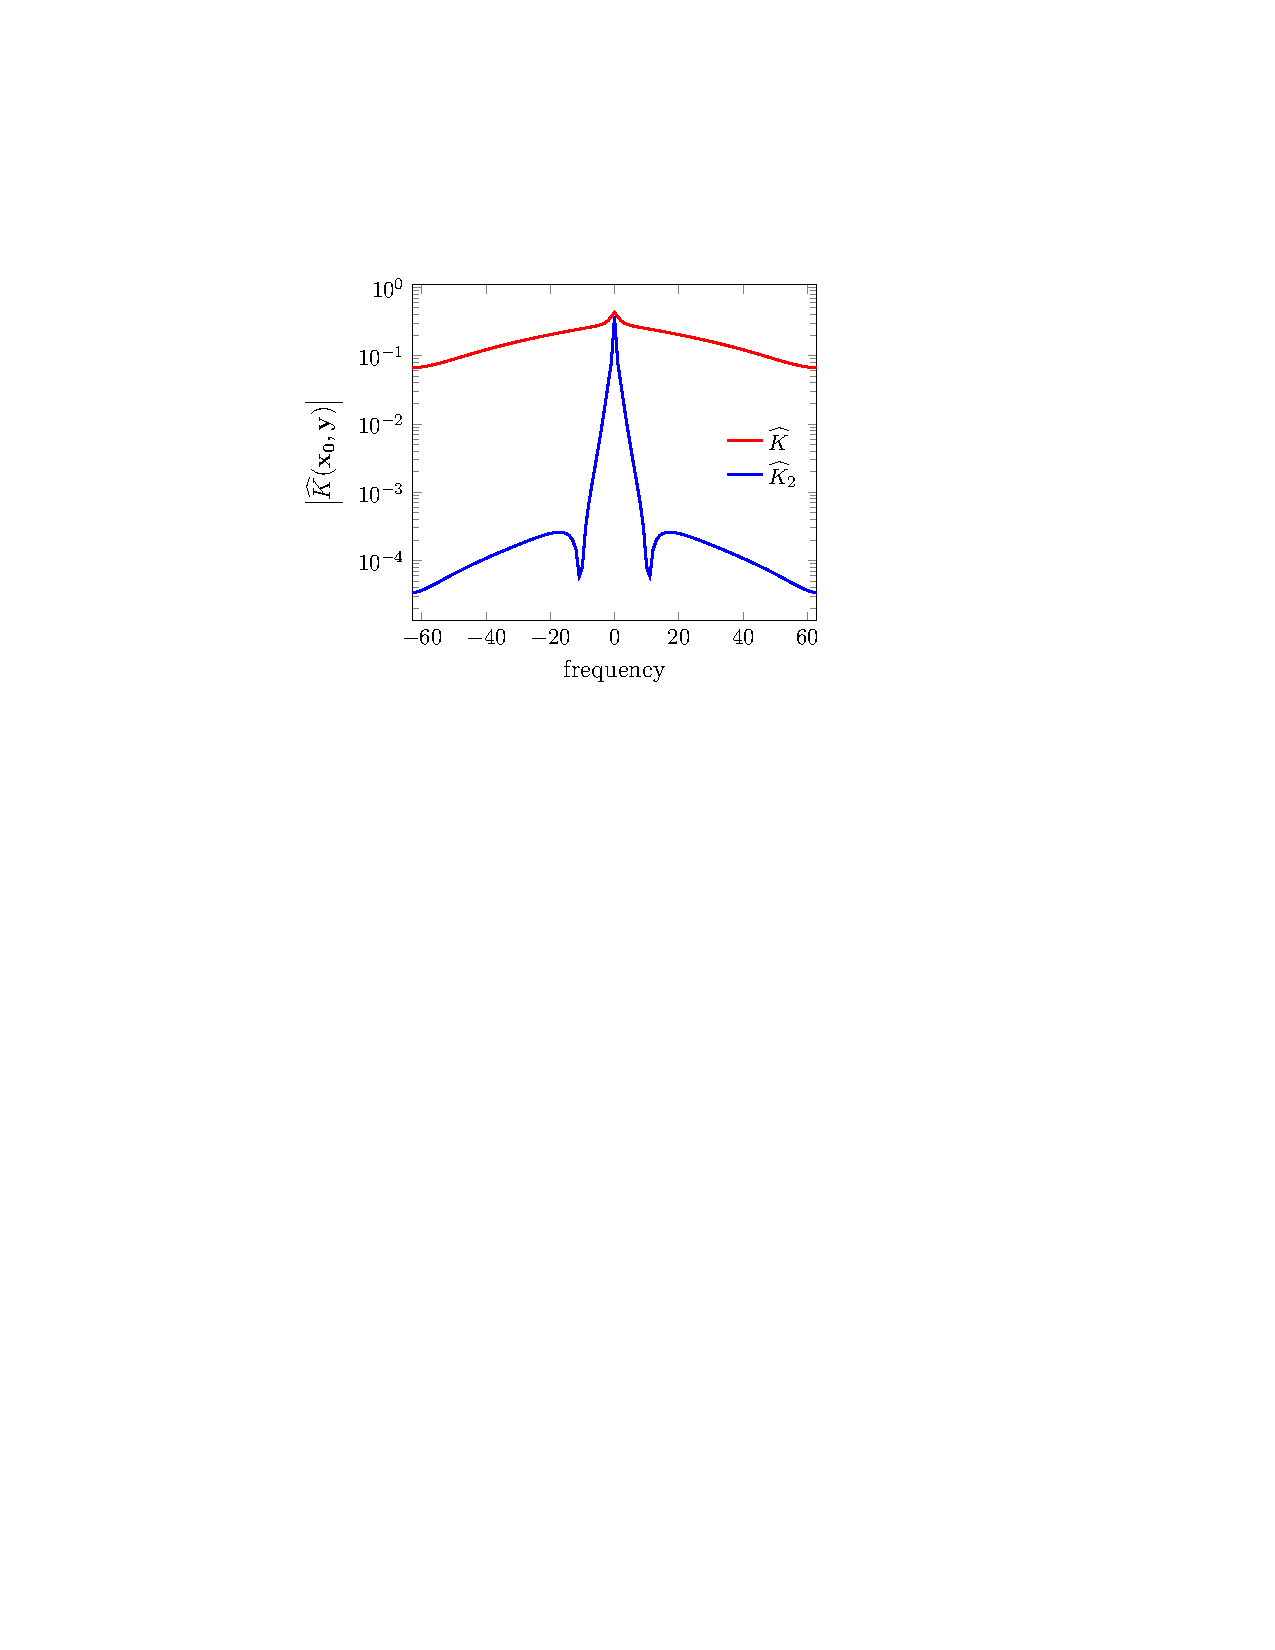
\includegraphics[width=2.4in]{figures/integrands}}
%\vspace*{-13pt}
%  \caption{{\footnotesize The Fourier modes of
%  $K(\mathbf{x_0},\mathbf{y})$ and $K_2(\mathbf{x_0},\mathbf{y})$ where
%  $|\mathbf{x_0}| = 0.99$, $\mathbf{y} \in \partial\Omega$, and
%  $\Omega$ is the unit disk. The trapezoid rule applied to the red
%  integrand has large amounts of error, but the trapezoid rule is much
%  more accurate when applied to the blue integrand. Since the difference
%  between the red and blue curves can be accurately computed with the
%  barycentric quadrature rule, the quadrature error applied to layer
%  potentials for the screened Laplace equation will be uniformly bounded
%  in $\Omega$.}}
%\label{fig:integrands}
%\end{wrapfigure}
Discretizations of carefully chosen BIEs can be solved with a
mesh-independent number of GMRES
iterations~\cite{cam-ips-kel-mey-xue1996}. Therefore, the required CPU
time is proportional to the cost of a matrix-vector multiplication that
can be performed in optimal or near-optimal time with the fast multipole
method (FMM)~\cite{fmm5} and its extensions~\cite{fmm1, fmm2, fmm3,
fmm4, fmm6, fmm7, fmm8}. PI BQ is experienced with applying FMMs for the
Stokes equation~\cite{qua-bir2014, bys-sha-qua2020} and the screened
Laplace equation~\cite{kro-qua2011, qua2011}.  Alternatively, fast
direct solvers avoid iteration~\cite{fds2, fds3, fds4, fds5, fds6, fds7,
ho2016cpam1, minden2016, minden2017siammms}, but often require a large
amount of computational overhead, and this makes them less practical for
problems with moving geometries. Alternatively, fast direct solver
techniques can be used to develop efficient preconditioning strategies
such as the inverse Fast Multipole Method (IFMM)~\cite{cou-pou-dar2017}.
PI BQ used the IFMM to precondition Stokes
equations~\cite{qua-cou-dar2018}. A suite of other preconditioners
including sparse approximate inverses~\cite{che2000} and
multigrid~\cite{hem-sch1981, sch1982} will be investigated.
%
%Nearly touching bodies is ubiquitous in self-assembly of amphiphilic
%particles, and this results in nearly-singular integrands. Quadrature
%methods for these integrands have received a lot of attention in two and
%three dimensions~\cite{alpert, kapur, sidi, duffy, bruno1, bruno2,
%davis_1984, graglia_2008, hackbusch_sauter_1994, jarvenpaa_2003,
%khayat_2005, schwab_1992, ying_2006, beale1, schwab_1992, ggq1, ggq2,
%ggq3, helsing_2008a, helsing_tutorial_2012, klockner2013jcp, qbx2,
%wala2019jcp, af2018sisc, siegel2018jcp, rachh2017jcp, ding2019arxiv,
%bar2014}. The trapezoid rule is the workhorse for two-dimensional BIEs
%since it achieves spectral accuracy when integrands are not
%nearly-singular~\cite{tre-wei2014}. To address nearly-singular
%integrands of two-dimensional BIEs, we will use a {\em barycentric
%quadrature rule} that only requires a slight modification of the
%trapezoid rule~\cite{ioa-pap-per1991}. In its current form, this method
%requires the layer potential to satisfy Laplace or Stokes
%equations~\cite{bar-wu-vee2015, chi-moo-qua2020}, but the PIs will
%extend the method to layer potentials for the screened Laplace equation.
%This will be done by recognizing that the fundamental solution of the
%screened Laplace equation can be decomposed as $K(\mathbf{x},\mathbf{y})
%= K_1(\mathbf{x},\mathbf{y}) + K_2(\mathbf{x},\mathbf{y})$, where
%$K_1(\mathbf{x},\mathbf{y}) = -\log|\mathbf{x} - \mathbf{y}|$ and
%$K_2(\mathbf{x},\mathbf{y}) = K(\mathbf{x},\mathbf{y}) + \log|\mathbf{x}
%- \mathbf{y}|$. Then, layer potentials involving
%$K_1(\mathbf{x},\mathbf{y})$ can be accurately computed with the
%barycentric quadrature rule~\cite{ioa-pap-per1991}, and layer potentials
%involving $K_2(\mathbf{x},\mathbf{y})$ can be accurately computed with
%the trapezoid rule since the kernel is bounded for all $\mathbf{x}$ and
%$\mathbf{y}$. The proposed method is demonstrated in
%Figure~\ref{fig:integrands}, where the amplitude of the Fourier modes of
%$K(\mathbf{x_0},\mathbf{y})$ and $K_2(\mathbf{x_0},\mathbf{y})$ are
%plotted. The quadrature error of the trapezoid rule is the sum of the
%unresolved Fourier modes.


% ----------------------------------------------------------------------
\subsubsection{Eliminating contact with adaptive time stepping and
repulsion}
\label{subsec:timeStepping}

A numerical issue when simulating the self-assembly of amphiphilic
particles is avoiding particle collision. The hydrophobic attraction
potential drives the amphiphilic particles towards one another and
this leads to physical contact in
finite time. Such particle collisions in a dense, rigid-body suspension
are a great challenge and can be a bottleneck in large-scale simulations.
We propose two algorithms to remedy this computational challenge:
high-order adaptive time stepping and repulsion forces.

PI BQ developed a high-order adaptive time stepping method for
hydrodynamic suspensions \cite{qua-bir2016}, and it has served as a
robust method to simulate processes including mixing and adhesion in
suspensions~\cite{qua-vee-you2019, kab-qua-bir2017}. The method uses
a single-step, high-order time stepping method and a computationally
cheap estimate of the error. The proposed work will use a spectral
deferred correction method~\cite{dut-gre-rok2000} since it iteratively
applies a low-order, single-step method to achieve high-order accuracy.
To estimate the error, at each time step, we will compute the total force
and torque of the system which is computationally cheap and physically
zero. PI BQ's experience is that error estimates based on physical
constraints such as force- and torque-free conditions appropriately
determine how the time step should be adjusted so that the dynamics are
resolved without the computational expense of techniques such as
embedded Runge-Kutta methods, step-doubling, and Richardson
extrapolation.

%%
%\begin{wrapfigure}[13]{r}{0.30\textwidth}
%\centerline{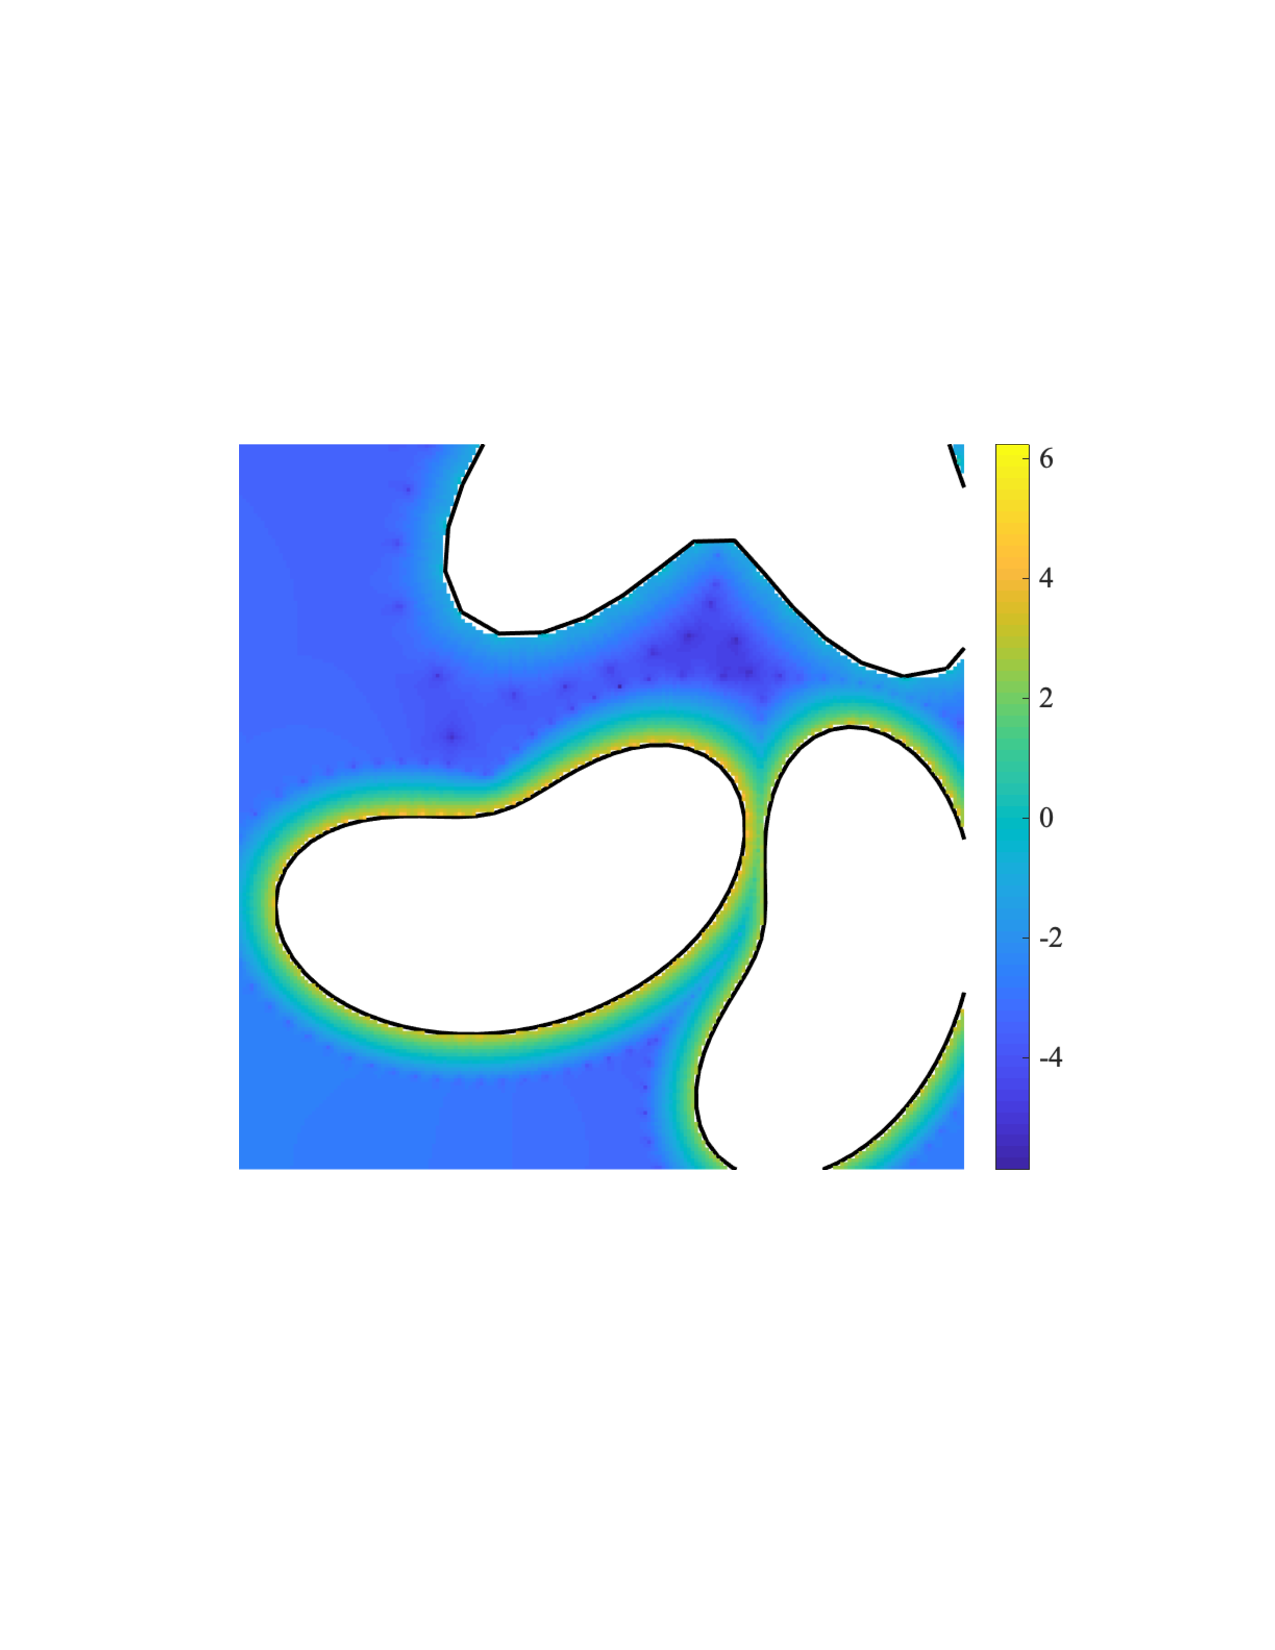
\includegraphics[width=0.29\textwidth]{figures/BIError.pdf}}
%  \vspace{-8pt}
%\caption{
%\label{fig:bierror}  
%\footnotesize The false color map shows how numerical quadrature of
%  layer potentials loses accuracy near the particle boundaries.  The
%  color bar is for $\log_{10}.$}
%\end{wrapfigure}
%%
Our previous work avoided particle contact through Lennard-Jones body
forces~\cite{Fu2018_SIAM}. Such steep, short-range, steric interactions 
introduce numerical stiffness and limit the time step size. To
remove this stiffness, we propose a geometry-based contact
method~\cite{har-pon-sor-zor2011}. This method has been applied to
vesicle suspensions~\cite{lu-rah-zor2017} and to rigid body suspensions in
two dimensions~\cite{bys-sha-qua2020} and three
dimensions~\cite{Yan2019}. These methods determine repulsion force by
solving a non-linear complementarity problem with a geometric constraint
that the configuration is non-overlapping. In this manner, contact is
avoided without the excessively small time steps required by stiff
Lennard-Jones forces.

%%-------------------------------------------------------------------------------
%\subsubsection{Novel reciprocal identities}
%\label{subsec:reciprocal}
%The force and torque formulas~\eqref{forceandtorque} use the
%hydrophobic stress along the particle boundaries. Unfortunately,
%layer potentials for $\nabla u$ involve hyper-singular integrals and
%this introduces large amounts of quadrature error on the particle
%boundaries (Figure~\ref{fig:bierror}). Therefore, it is useful to devise
%reciprocal identities for the force and torque on body $i$ that do not
%require integration along body $i$. One identity, that we have proved,
%is
%\begin{align}
%    \label{eq:reciprocal}
%{\bf F}_{\text{hydro},i} = \sum_{j \neq i} \int_{\partial P_i}[\boldsymbol{\sigma}_{ij} + \boldsymbol{\sigma}_{ji}]\boldsymbol{\nu}\,\dif S,\quad
%{\bf G}_{\text{hydro},i} = \sum_{j \neq i} \int_{\partial P_i} ({\bf
%  x}-\mathbf{a}_i) \times [\boldsymbol{\sigma}_{ij} +
%  \boldsymbol{\sigma}_{ji}]\boldsymbol{\nu}\,\dif S, 
%\end{align}
%for $i=1,\ldots,N$. Here, $u_i$ is the solution of the screened Laplace
%equation when only the contribution from particle $i$ is considered and
%$\boldsymbol{\sigma}_{ij} = \rho^{-1} u_iu_j \mathbf{I} +
%\rho\left((\nabla u_i \cdot \nabla u_j) \mathbf{I} - 2 \nabla u_i
%\otimes \nabla u_j\right)$. Equation~\eqref{eq:reciprocal} does not
%require knowledge of $\nabla u$ on particle boundary $i$, and this is
%enormously beneficial for calculating the hydrophobic force and torque.
%
%% ----------------------------------------------------------------------
%\subsubsection{Fluctuating hydrodynamics}
%\label{subsec:fluctuating}
%Once algorithms that address quadrature, adaptive time stepping, and
%contact are implemented, we will embark on incorporating fluctuating
%hydrodynamics that are especially important at scales of amphiphilic
%particles. Bao et al.~\cite{Bao17,Bao18} developed two-dimensional BIE
%formulations for Brownian rigid bodies. To satisfy the covariance of the
%rigid body velocities, they use an ill-conditioned, first-kind integral
%equation method. The proposed work will consider a layer potential
%formulation that has much better conditioning properties. This strategy
%was attempted in~\cite{Bao18}, but they claim that a necessary
%regularization of the covariance matrix leads to a drastic loss of
%accuracy in numerical fluctuation-dissipation balance. However, only one
%regularization strategy was considered, and as PI BQ has shown in
%previous work, the regularization choice significantly affects the
%resulting physics~\cite{ong-chr-qua2017}. Therefore, different
%regularization strategies will be investigated with the goal of finding
%well-conditioned BIE formulations that control the accuracy of the
%fluctuation-dissipation balance.



\subsection{Specific Aim 3: Self-assembly of Janus particles in ionic solutions}
\label{subsec:specific_aim_3}

\subsubsection{Dynamics of a single Janus particle in ionic solutions}
In experiments, Janus particles are often immersed in a solution of ions \cite{ChenWhitmer2011_Sci} or surfactants \cite{}.
In electrolytic solutions the interaction between salt and Janus particle gives 
rise to a slip velocity (on the particle surface) that depends on the ion distribution and the zeta potential \cite{BayatiJCP2016} 
(the potential difference between the Janus particle surface and the surrounding conducting fluid).
The short-range interactions between Janus particles depend on the salt concentration:
At very low salt concentrations, Janus particles repel one another electrostatically, whereas at high salt concentration, van der Waals
forces cause Janus particles to aggregate irreversibly \cite{Goodwin2019}. At intermediate concentrations of monovalent salt, Janus particles are found to self assemble in the form of a small number of elemental units of building blocks \cite{Chen2011_Science}. 
%
\begin{wrapfigure}[11]{l}{0.47\textwidth}
\centerline{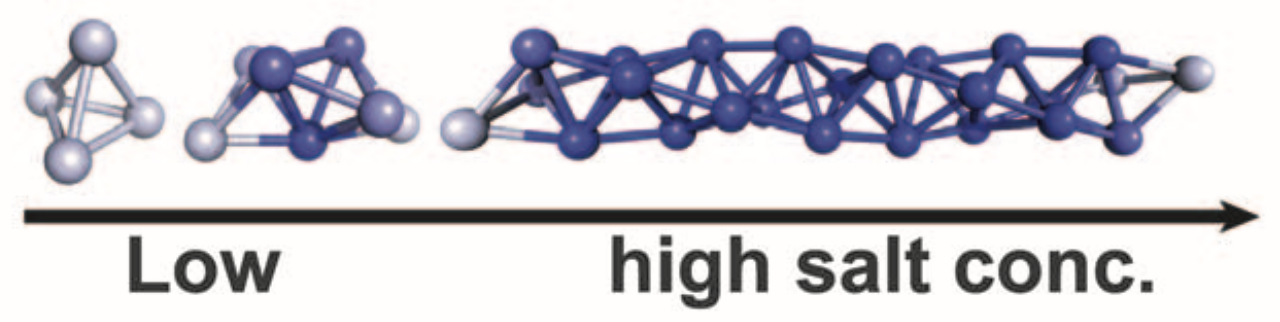
\includegraphics[width=0.46\textwidth]{Figures/fig2A_Chen2011_Science}}
  \vspace{-5pt}
\caption{\label{fig:helices_of_JPs} \footnotesize Formation of helices of Janus particles as salt concentration increases \cite{Chen2011_Science}.}
\end{wrapfigure}
%
Figure~\ref{fig:helices_of_JPs} shows that Janus particles can self-assemble into a helix at high concentration of monovalent salt (NaCl) when the density of Janus particles is low to moderate. At high density, JPs are found to form wormlike structures

The Stokes equations in~\eqref{eq:stokes} are modified to incorporate the transport of ions as
\begin{equation}
\label{eq:stokes}
\begin{aligned}
  &-\mu \Delta \mathbf{u} + \nabla p = \Delta\psi\cdot\nabla\psi, \quad \mathbf{x} \in \Omega, \qquad
  \nabla \cdot \mathbf{u} = 0,  \quad \mathbf{x} \in \Omega,\\
  &\delta^2\Delta\psi = -\frac{1}{2}\left(n_+-n_-\right),\qquad
  \frac{\partial n_{\pm}}{\partial t} + \nabla\cdot{\bf j}_{\pm} = 0,\\
  &{\bf j}_{\pm} = -\nabla n_{\pm} \mp n_{\pm} \nabla\psi + Pe n_{\pm}\mathbf{u}.
\end{aligned}
\end{equation}
The screen length $\rho$ is now a function of the ion concentrations: $\rho = \rho(n_+,n_-)$. 






\subsubsection{Electromechanical effects on the dynamic assembly of amphiphiles \label{subsubsec:em_effects}}
In recent experiments~\cite{FaizEtAl2019_SoftMatt}, membrane bending
rigidity was determined as a function of lipid composition from 0 to 100
mol $\%$ of charged lipids using flicker spectroscopy of the shape
fluctuations of a giant unilamellar vesicle (GUV).
%the bending rigidity is determined as a
%function of lipid composition from 0 to 100 mol $\%$ of charged lipids
%in recent experiments~\cite{FaizEtAl2019_SoftMatt}---
Membrane bending rigidity increases with increasing lipid surface
charge, but decreases with increasing salt concentration in the bulk
solution due to the screening of the lipid surface charge. This
result agrees
with several theoretical models~\cite{Kralchevsky1996_JCIS,
May1996_JChemPhys, LoubetEtAl2013_PRE} that also assume the quadratic
form of the elastic energy density in the presence of surface charge and
bulk charge~\cite{DuplantierGoldstein1990_PRL, Winterhalter1992_JPC}. As
the electrostatic interaction is non-local in nature, we expect that the
controversy of the HK elastic energy form (see
\S\ref{subsec:specific_aim_1}) would worsen in the presence of
electrostatic interactions and electrokinetics. The PIs will extend the
approaches in \S\ref{subsec:specific_aim_1} to charged lipids to
calculate the bending moduli and compare against the experimental
results in~\cite{FaizEtAl2019_SoftMatt}. We propose to incorporate an
explicit surface charge on each particle boundary $P_i$ and compute the
electrostatic potential as a functional of particle configuration.
Adding the electrostatic force to the hydrophobic attraction force
between particles, we will assess the dependence of elastic moduli on
electric charges using the methods described in
\S\ref{subsec:specific_aim_1}. Results from these proposed calculations
will provide further comparisons and validations of the HAP model
against the continuum mechanics.

Once the effects of lipid charges on the moduli are verified, the PIs
propose to examine how to use an external electric field to control the
amphiphilic self-assembly in solvent. PI YNY has a track record of
working on electrohydrodynamics of an elastic, inextensible membrane
using both asymptotic analysis~\cite{Nganguia2013_PRE, Young2014_JFM,
Young2015_PoF} and numerical simulations~\cite{Nganguia2015_CiCP} and
will work with both PIs RR and BQ to extend the HAP model to study the
electromechanical effects on the assembly of amphiphile. Results from
this research will yield a quantitative understanding of how to utilize
an electric field to achieve optimal control of assembly of amphiphiles
in solvent.





\begin{figure}[!]
\begin{center}
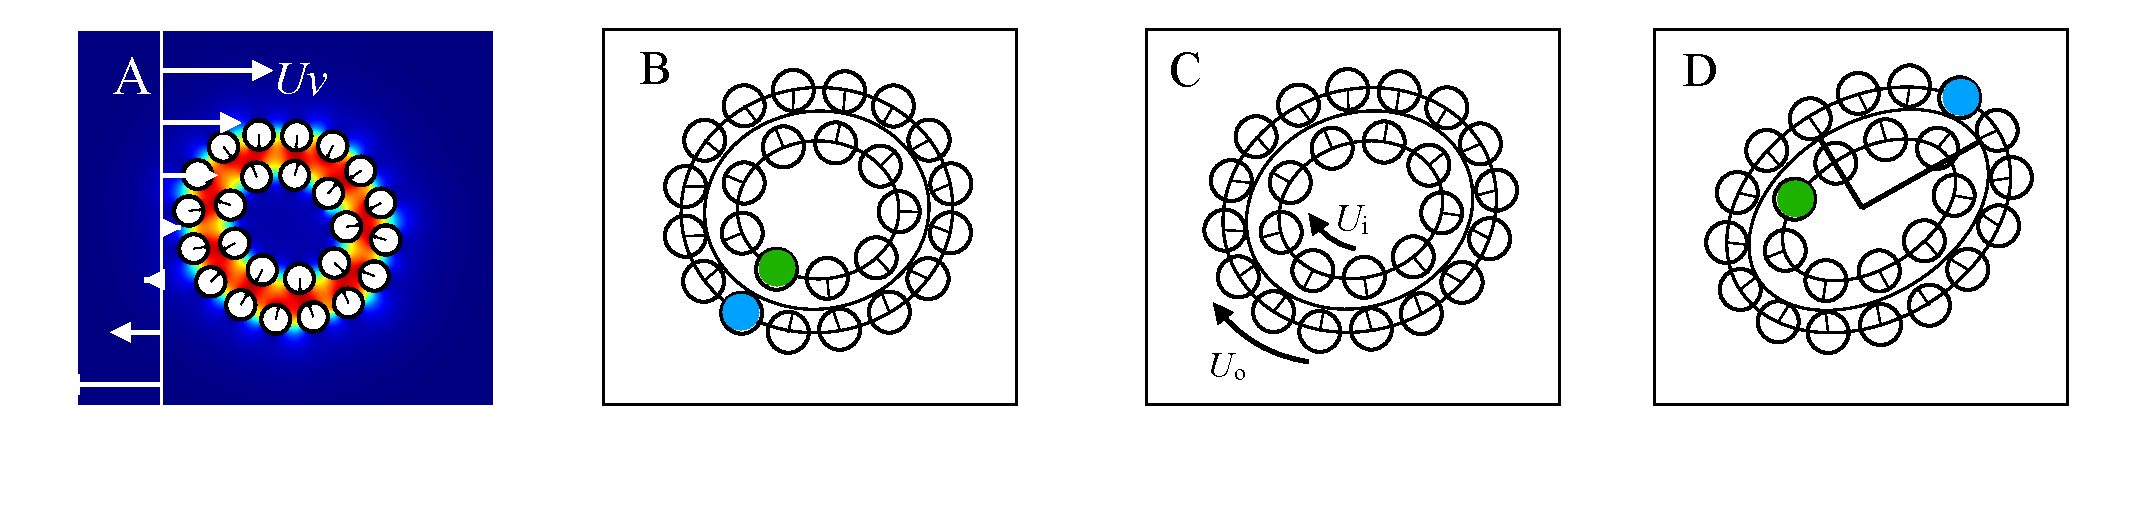
\includegraphics[width=1\textwidth]{figures/PW_fig1A-D.pdf}
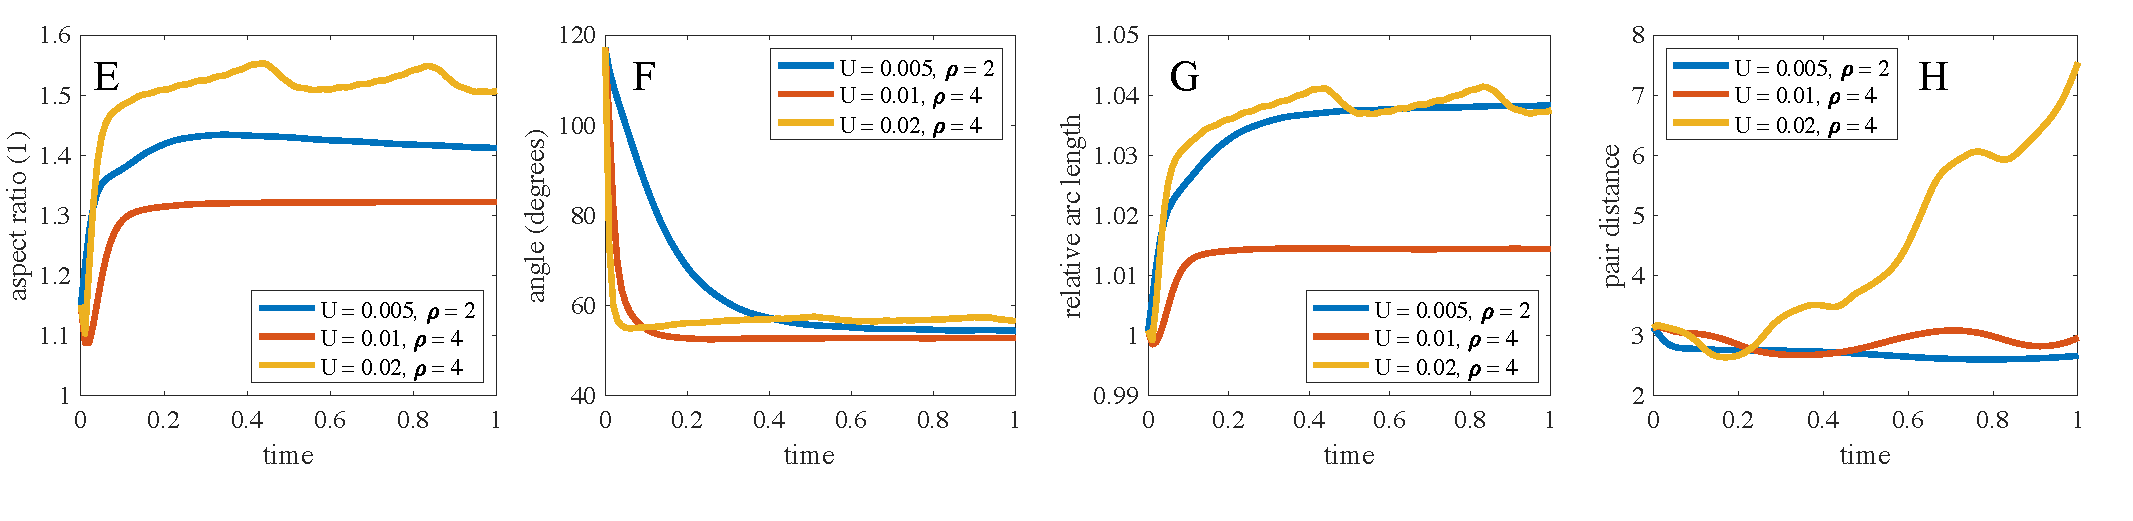
\includegraphics[width=1\textwidth]{figures/PW_fig1E-H.pdf}
\end{center}\vspace{-0.3in}
\caption{(A) A vesicle formed by amphiphilic particles in shear flow,
  and the tank-treading motion (B)--(D). The separation of particle
  pairs in (B) and (C) illustrate inter-leaflet slip.  (E)--(G)
  Tank-treading reaches a steady state in elliptical aspect ratio,
  major-axis angle, and circumference.}
\label{fig:tanktreading}
\end{figure}
\section{Preliminary Work on Two-dimensional Vesicle Hydrodynamics in Shear Flow\label{sec:preliminary_work}} 
%The motion of vesicles in shear flow is an important
%problem in the applied mathematics because simulations can reveal mechanical
%properties of membranes and lead to an enhanced understanding of 
%deformable particle laden flows \cite{Sinha15}. 
%
To implement a vesicle in shear flow in the context of hydrophobic potentials and mobility problem, 
we consider a shear flow in the far-field $\mathbf{u}_{\infty} = Uy\mathbf{i}_x$ in the direction of the $x$-axis
(Figure \ref{fig:tanktreading}A).
%
%This field satisfies the linear Stokes system but does not give rise to a rigid motion at the particle interfaces. 
%To have a rigid motion, we change variables $\mathbf{u} = \tilde{\mathbf{u}}+ \mathbf{u}_{\infty}$ and 
%for the new field $\tilde{\mathbf{u}}$ vanishing at infinity we let 
%$\tilde{\mathbf{u}}|_{\partial P_i} = \mathbf{v}_i + \boldsymbol{\omega}_i \times (\mathbf{x} - \mathbf{a}_i)$ 
%where $(\mathbf{v}_i,\boldsymbol{\omega}_i)$ are the unknown translation and angular velocities of the 
%$i$th particle $P_i.$  
%
%\begin{wrapfigure}[17]{l}{0.4\textwidth}
%\centerline{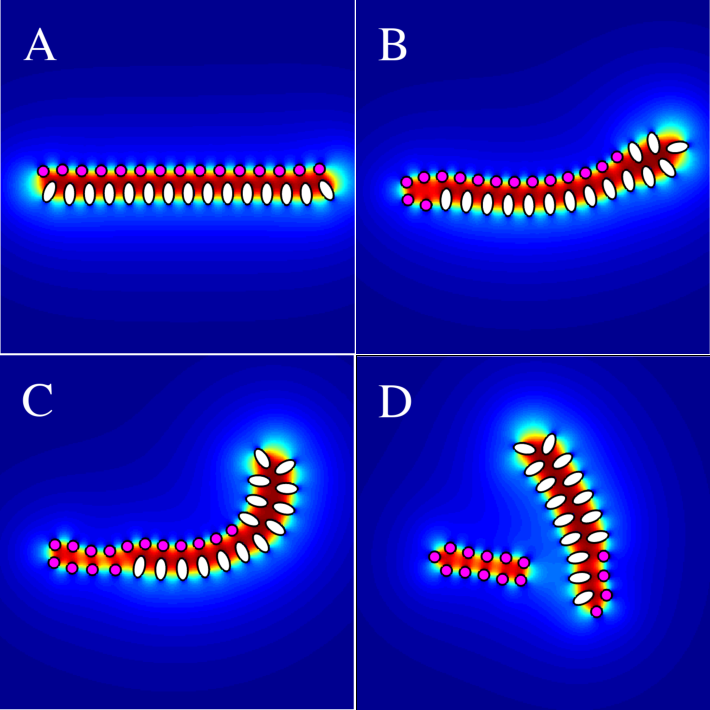
\includegraphics[width=0.4\textwidth]{figures/PW_fig2.pdf}}
%\caption{\label{fig:demixing} An initial assembly of small and 
%large particles spontaneous segregates into two smaller bodies. }
%\end{wrapfigure}
The HAP simulations show vesicle tank-treading. Under the external shear flow, the initially circular 
vesicle rotates in the clockwise direction. As the rate of rotation increases, the vesicle approaches
a steadily tank-treading ellipse. In Figure \ref{fig:tanktreading}B-D, the solid curves are ellipses fit to the particle centers
and midplane respectively. In the non-dimensionalized system, the particles have diameter 2, on the order of $\rho,$ 
and the vesicle diameter is about 14. 
%\todo[inline]{missing units. nm?}
%
\begin{wrapfigure}[12]{r}{0.2\textwidth}
\centerline{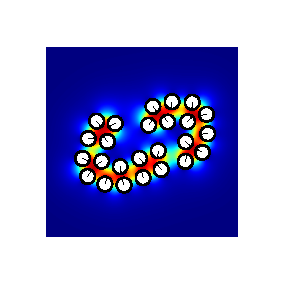
\includegraphics[width=0.2\textwidth]{figures/PW_fig5.pdf}}
\caption{\label{fig:rupture} Rupture of tank-treading vesicle under strong shear flow.}
\end{wrapfigure}
%
Figure~\ref{fig:tanktreading}E shows the aspect ratio of the major to minor axes reaching an equilibrium value in the 
red and blue curves, yet oscillating in the high-shear rate (yellow) curve.
The tank-treading vesicle elongates and becomes more horizontal 
with an increase in flow rate or 
with a decrease in stiffness (effected by decreasing $\rho = 4$ to $\rho = 2$). 


For large shear flow rates, there is an increase in arc length. Here arc length
refers to the the mid-plane circumference. Thus,
some of the external force is going into stretching the vesicle--the other
part is going into bending and viscous dissipation. From our experiments, 
we find that the vesicle ruptures once stretching exceeds about 5 \%
(see Figure \ref{fig:rupture}).
Finally, movies of the tank-treading motion show a slip velocity
between the outer and inner leaflets Figure \ref{fig:tanktreading}G. We have illustrated this 
by tracking the distance between two reference particles in the inner and outer leaflet
(Figure \ref{fig:tanktreading}B \& D, green and blue particles). 
With moderate shear rates or greater adhesion, the particle pair moves in tandem
(in Figure \ref{fig:tanktreading}H, blue and red curves, their distance is more or less constant). 
For a large shear rate, the particle separates as the two leaflets slide against one another. 



%\begin{wrapfigure}[12]{r}{0.2\textwidth}
%\centerline{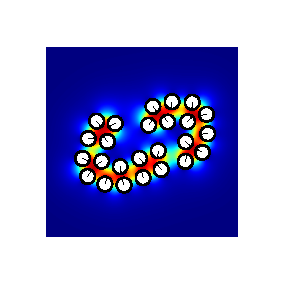
\includegraphics[width=0.2\textwidth]{figures/PW_fig5.pdf}}
%\caption{\label{fig:rupture} Rupture of tank-treading vesicle under strong shear flow.}
%\end{wrapfigure}
There are a number of advantages to using our particle based approach.
For one, the HAP theory automatically accounts for the existence of multiple phases. 
For example, we can vary lipid length, spontaneous curvature and bending rigidity 
by introducing differentiating particle shapes and hydrophobic boundary conditions (Figure \ref{fig:demixing}).
Continuum theory deals with multiple phases through additional surface densities that must
then satisfy specialized transport equations \cite{Lowengrub07,MikuckiZhou17}. 
As illustrated in Figure \ref{fig:tanktreading}, the particle
based approach supports inter-leaflet slip, and this can be used to determine inter-leaflet
and in-plane shear viscosities. 
%





\section{Relevant Results from Prior NSF Support}
\noindent {\bf Rolf Ryham}: no prior NSF support.

\noindent
{\bf Yuan-Nan Young}: {\em NSF-DMS-1222550, Mathematical and
experimental study of lipid bilayer shape and dynamics mediated by
surfactants and proteins}, \$212,603, 9/15/2012 - 08/31/2016 (with
no-cost extension), PI. {\em Intellectual merit:} The focus of this
grant is modeling the interaction between a pure lipid bilayer membrane
with surfactant, cholesterol, and protein.
%Hence, there is no overlap between these grants and the current proposal.

%YNY and collaborators have studied (1) asymmetry of lipid bilayer due to its interaction
%with proteins and surfactants, (2) the electrohydrodynamics of a LBM under an
%electric field, and (3) the coupling between LBM dynamics and a transmembrane protein,
%such as a mechanosensitive channel. 

\noindent
{\it Broader impacts:} 
One PhD student (Szu-Pei Fu) was funded to work with YNY, and work has
resulted in seven papers~\cite{Nganguia2013_PoF, Nganguia2013_PRE,
Young2014_JFM, Young2015_PoF, Nganguia2015_CiCP,
Pak2015_PNAS,fu2015pre}. YNY has been actively involved with promotion
of underrepresented students at NJIT. One PhD student, Herve Nganguia,
is now an Assistant Professor at Towson University. YNY has taught a
broad spectrum of courses in fluid mechanics and applied math modeling.

\noindent
{\bf Bryan Quaife}: {\em NSF DMS-2012560, Erosion, Transport, and
Dispersion in Granular and Porous Media}, \$249,636,
08/01/2020--07/31/2023, PI. {\em Intellectual Merit:} The goal of this
research is to develop high-order numerical methods to
simulate hydrological processes including erosion.

\noindent
{\it Broader impacts:} 
A third-year PhD student (Jake Cherry) has been assigned to this
project. One paper will be submitted before December
2021~\cite{che-lin-her-qua2022}.

\section{Project Management, Collaboration Plan, and Schedules of
Research Tasks}
\setlength{\parindent}{0pt}
% N.B. wrapfigure is not compatible with \noindent.

\begin{wrapfigure}[10]{r}{0.4\textwidth}
  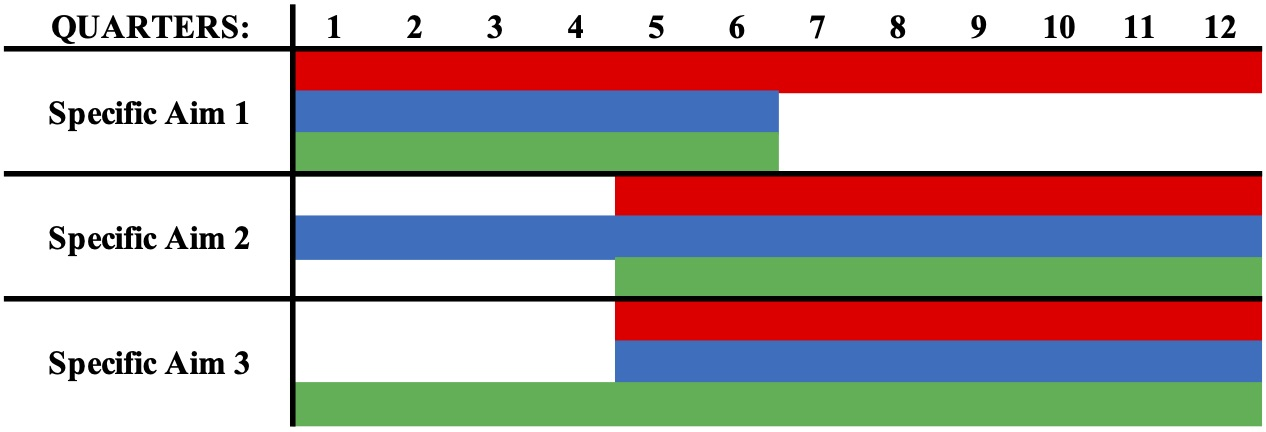
\includegraphics[width=0.4\textwidth]{figures/gantt.jpg}
  \caption{\label{fig:schedule} Schedule for the proposed work, measured
  in quarters from the beginning of the project. The lead PI of each
  Specific Aim will be RR (red), BQ (blue), and YNY (green).}
\end{wrapfigure}


\begin{comment}
\begin{wrapfigure}[11]{r}{0.56\textwidth}
\vspace{-19pt}
%\definecolor{barblue}{RGB}{51,102,254}
%\renewcommand\sfdefault{phv}
%\renewcommand\mddefault{mc}
%\renewcommand\bfdefault{bc}
%\sffamily
\begin{ganttchart}[
    canvas/.append style={fill=none, draw=black!5, line width=.75pt},
        x unit =4.5mm,
        y unit chart =\baselineskip,
    hgrid style/.style={draw=black!5, line width=.75pt},
    vgrid={*1{draw=black!5, line width=.75pt}},
    title/.style={draw=none, fill=none},
    title label font=\bfseries\footnotesize, % numbers across the top
    title label node/.append style={below=3pt},
    include title in canvas=false,
    bar label font=\mdseries\footnotesize\color{black!70}, 
    % titles across the left
    %bar label node/.append style={left=2cm},
    bar/.append style={draw=none, fill=blue},
    bar incomplete/.append style={fill=blue},
    bar progress label font=\mdseries\footnotesize\color{black!70},
    milestone label font=\mdseries\small\color{black!70},
        milestone left shift =0.9,
        milestone right shift =0.1,
        % Don't draw group bars
        group height =0,
        group peaks height =0,
        group label font =\bfseries\small,
]{1}{12}
\gantttitle[
    title label node/.append style={below left=3pt and -6pt}
]{QUARTERS:\quad1}{1}
\gantttitlelist{2,...,12}{1} \\
%\ganttgroup{Tasks\hfill}{1}{12}\\
\ganttbar[bar/.append style={fill=red}]{Specific Aim 1}{1}{12} \\
\ganttbar[bar/.append style={fill=blue}]{Specific Aim 2}{1}{12}\\
\ganttbar[bar/.append style={fill=green}]{Specific Aim 3}{1}{12}\\
\ganttbar[bar/.append style={fill=black}]{Program Management}{1}{12}
\ganttbar[bar/.append style={fill=magenta}]{}{4}{4}
\ganttbar[bar/.append style={fill=magenta}]{}{8}{8}
\ganttbar[bar/.append style={fill=magenta}]{}{12}{12}
\end{ganttchart}
\vspace{-10pt}
\caption{Schedule for the proposed work, measured in quarters from the
  beginning of the project. The lead PI of each Specific Aim will be RR
  (red), BQ (blue), and YNY (green). Project management will be
  continuous (black), but we anticipate extra attention will be
  necessary to align objectives in quarters 4, 8, and 12 (magenta).}
\label{fig:schedule}
\end{wrapfigure}
\end{comment}
\textbf{Project management}: 
%
The success of the proposed research requires complementary expertise
and collaborative efforts in physics, applied mathematics, algorithms,
and computing. PI RR has been working on mathematical modeling with a
strong analytical background. PI YNY has been working on many areas of
computational fluid dynamics and applications to math biology for many
years. PI BQ has been working on integral equation methods, fast
algorithms, and their applications to fluid dynamics for many years.
Their recent collaborative work on the HAP model in two
dimensions~\cite{FuQuRyYo22} has provided a solid foundation for the
proposed research.

\smallskip

\textbf{Collaboration plan}: 
%
The management responsibility of this collaborative research will reside
with the lead PI (RR) for this endeavor. The research work is structured
to meet the tasks discussed in \S\ref{sec:proposed-work}. The PIs,
postdocs, and students will meet frequently on Zoom and in person when
possible.
%During the pandemic, the three PIs will meet weekly on Zoom
%for a research meeting.
Once the pandemic is under control, PI RR and PI
YNY will conduct biweekly meetings in person, with PI BQ Zoom in from
Florida. The PIs will share software packages, paper sources, and
references on a common \textsf{Git} repository. The resulting software
packages will be posted on the \textsf{Github} software repository.
%
%\smallskip
%
\textbf{Research Schedule:} The detailed schedule for the proposed work
is shown in Figure~\ref{fig:schedule}. Each PI will spearhead a
different Specific Aim, and program management will happen
throughout, with special coordination taken in quarters 4, 8, and
12.





\newpage
\setcounter{page}{1}
\addcontentsline{toc}{section}{Bibliography}
\bibliographystyle{abbrvnat}
%
\bibliography{refs}



\end{document}
